%--- Chapter 1 ----------------------------------------------------------------%
\chapter{Introduction}
% \section{Chapter One Section One}
% \subsection{Chapter one section one sub-section one}
% \newline
~\\
% Test: including section 1.1 into the file
% \newline
% \begin{equation}
% y = a*x + b
% \nabla 
% \end{equation}

% This is a sample citation: \cite{schwartz_overview_2012}.
\section{Introduction to earthquakes}
Every year, around ~20,000 earthquakes happen around the world. Some are not noticeable, while others cause huge damage to property and life.
Earthquakes have been recorded for thousands of years. 
% and they are considered as signs or punishments to humans from supernatural powers in many civilizations.
Over the past centuries, with advancements in mathematics, physics, geology, and other natural sciences, we have a more structured understanding of earthquakes today.

An earthquake represents a complex process of fault slip and energy release within the Earth's crust, driven by tectonic forces and resulting in the shaking of the ground and potentially causing damage to structures and infrastructure. 
An earthquake occurs due to the sudden release of accumulated stress along a fault line, resulting in rapid movement known as fault slip. This movement can be described in terms of several key components:

\subsection{Fault rupture}
The earthquake begins with the rupture of the fault, where the stress accumulated along the fault plane exceeds the strength of the rocks, causing them to fracture and slide past each other. This rupture initiates the seismic event.

\subsection{Sesmic waves} 
As the fault slips, it generates seismic waves that propagate through the Earth's crust and outward from the fault.
These weaves transmit energy in the form of vibrations, which cause the ground to shake.

\subsection{Slip motion}
Slip motions are the noticeable components of an earthquake movement.
The fault slips during an earthquake and involves two types of movements
\begin{itemize}
    \item Primary slip (seismic slip): This is the sudden and rapid movement along the fault plane during the initial rupture. It is usually associated with the intense shaking and damage from the earthquakes
    \item Afterslip: Following the primary slip, there may be additional movement along the fault. This ongoing slip can continue for days, weeks, or even months after the initial earthquake.
\end{itemize}

\subsection{Displacement}
The amount of fault slip during an earthquake is measured in terms of displacements. 
This is the distance that one side of the fault moves relative to the other.
Displacement can be horizontal, vertical, or both.


\section{Seismic and aseismic slip}
The slip motion of an earthquake can further be classified into seismic and aseismic slips.
\subsection{Seismic slip}
Seismic slip refers to the sudden release of accumulated tectonic stress along a fault plane, resulting in what is often called an earthquake.
This type of fault slip is characterized by rapid and dynamic movement, which generates seismic waves propagating through Earth's crust, causing ground shake and potential damages to infrastructures.
Seismic fault slip occurs when stress accumulated along a fault exceeds the frictional resistance holding the fault surface, causing sudden slip and rupture.
\subsection{Aseismic slip}
Aseismic slip, also known as creep or slow slip, refers to gradual continuous movement along a fault plane without generating significant earthquakes and seismic waves.
Unlike seismic slip, aseismic slip occurs at rates that are usually much slower and may not produce noticeable ground shaking or seismic activity.
Aseismic slip represents a steady release of tectonic stress along the fault, often occurring in between larger seismic events.
However, the stress could still increase during seismic slip, leading to seismic slip in the future.
Aseismic slip can contribute to the overall deformation of the Earth's crust and could play a potential role in seismic hazard assessments and forecasting.
Modeling the behavior of aseismic slip has been essential in order to understand the nucleation of seismic slip and the mechanism behind multiple cycles of earthquakes.

\subsection{Budget}
In the context of seismology, budget refers to the distribution and allocation of accumulated tectonic stress or energy between seismic and aseismic slip events.
Understanding the balance between seismic and aseismic slip budgets is important for assessing seismic hazard and fault behavior.
It helps researchers and geoscientists to understand the mechanisms governing fault movement and stress release to forecast earthquakes. A detailed discusssion on principles of fault slip budget determination and observational constraints on seismic and aseismic slip can be found in this review paper\citep{annurev:/content/journals/10.1146/annurev-earth-060614-105302}.


\section{Velocity weakening/strengthening}
Understanding the frictional behavior along the fault is the key to understanding the different behaviors of seismic and aseismic slip.
Friction is often associated with the velocity of the fault displacement.
Based on the different responses to sliding velocity, regions on the fault can be classified into two types: velocity weakening and velocity strengthening.
\subsection{Veclocity weakening region}
In a velocity weakening region, the frictional resistance between the fault surfaces decreases with an increasing slip velocity.
In other words, as the sliding velocity along the fault increases, the friction strength decreases.

This phenomenon is crucial in earthquake dynamics because it promotes the instability of the fault and facilitates the rapid release of accumulated stress during earthquakes.
When the friction resistance decreases with increasing velocity, the fault becomes more prone to slip suddenly and can generate earthquake waves.
Velocity weakening regions are often associated with materials or conditions that exhibit unstable slip behavior, such as fault gouge, pore pressure, and fluids.

\subsection{Velocity strengthening region}
In contrast to velocity weakening region, a velocity strengthening region is characterized by an increase in frictional resistance with increasing slip velocity.
The velocity strengthening regions tend to promote stable fault behavior, resisting slip and preventing rapid release of stress that leads to earthquakes.
Instead, fault slip in these regions may occur aseismically.

Velocity strengthening is typically observed in the shallow crust and at greater depths where ductile deformation mechanisms dominate. 
Conditions such as high confining pressure and high temperature, which promote stable creep and plastic deformation, contribute to this behavior.
\section{Rate-and-state friction law}
% \subsection{Rate-and-state friction law}
Since the recognition that earthquakes probably represent frictional slip instabilities in the 1960s, interest in determining frictional properties has been increased.
The stability of frictional sliding depends on whether frictional resistance increases or drops during slip.
Laboratory experiments have shown that frictional sliding is mainly a rate-dependent process in a steady-state regime with constant stress and steady velocity.
Due to this, a state variable needs to be introduced to describe
\begin{itemize}
    \item the transient behavior observed in non-steady-state experiments, denoted as $a$. This parameter presents the direct effect of the fault slip rate on the frictional resistance. In many rate-and-state friction laws, an increase in slip rate tends to increase the frictional resistance, and $a$ quantifies the strength of this effect. A higher value of $a$ means that the frictional resistance increases more rapidly with slip rate
    \item healing in hold-and-stick experiments denoted as $b$. This parameter represents the evolutionary effect of the fault slip on the frictional resistance. It quantifies how the frictional resistance evolves over time due to slip history. A positive value of $b$ means that slip tends to decrease the frictional resistance over time, making fault slip easier in the future. A negative value of $b$ implies the opposite, where slip tends to increase the frictional resistance over time, making fault slips harder.
\end{itemize}
These parameters are often determined empirically through laboratory experiments or field study. They play a crucial role in modeling the dynamics of earthquakes.
The formulation of such rate-and-state variable has significantly simplified the impacts of several parameters from rheology on the slip rate, which enables the development of numerical models to simulate earthquake cycles.

For most materials, it has been revealed by laboratory experiments on frictional sliding that the following conditions exist:

\begin{itemize}
    \item The resistance to sliding depends on the sliding rate at steady rate, along with a logarithmic dependency of the coefficient of friction on the slip rate.
    \item The resistance to sliding increases to a transient peak value when the imposed slip rate is suddenly changed, with the peak value being a logarithmic function of the slip rate.
    \item The friction coefficient is approximately a linear function with the logarithmic of the time in hold-and-slip experiments.
\end{itemize}

Laboratory measurements at slow sliding rates can be reproduced relatively well with a rate-and-state formalism on the order of microns per second.
Various laws have been proposed \citep{https://doi.org/10.1029/JB084iB05p02161, https://doi.org/10.1029/JB084iB05p02169,https://doi.org/10.1029/JB088iB12p10359,annurev:/content/journals/10.1146/annurev.earth.26.1.643}.

One common such law is called the aging law
\begin{align}
    \mu &= \mu_* + (a - b) \ln \frac{V}{V_*} \\
    \frac{d\theta}{dt} &= 1 - \frac{V\theta}{D_c}
\end{align}
At steady state, the law is purely rate dependent
\begin{equation}
    \mu_{ss} = \mu_{*} + (a - b) \ln \frac{V}{V_*}
\end{equation}

For a single-degree-of-freedom system such as a spring-and-slider system, the stability analysis shows that the slip can be stable only if $a - b > 0$ and that unstable slip requires that $a - b < 0$  
%(\citep{Priestley_1990}). 
For unstable slip to occur, it requires $a - b$ that is smaller than a critical negative value, defining an intermediate domain of conditional stability.
For a crack with size L embedded in an elastic medium with shear modulus $G$, the condition for unstable slip is 
\begin{equation}
    a - b < - \lambda \frac{GD_c}{L\sigma_n'}
\end{equation}
where $\lambda$ is on the order of unity. 
$\sigma_n'$ is the effective normal stress with $\sigma_n' - \sigma_n - P$ where $P$ is pore pressure.
In the limit when the pore pressure becomes near lithostatic, the critical value becomes infinite.
This implies that high pore pressure should promote stable slip through the reduction of the effective normal stress.
The rate-and-state friction and many definitions here are important concepts in the earthquake cycle simulations that are going to be discussed in later chapters.

\citep{}
% \subsubsection{Chapter one section one sub-section one sub-sub-section one}i
\section{SEAS project}
The progress in understanding earthquake behaviors from rate-and-state friction laws makes numerical modeling of earthquakes possible. Many numerical models have been proposed to understand earthquake behaviors from single earthquakes to multiple earthquake simulations.

\subsection{The limits of dynamic ruptures and earthquake simulators}
For individual earthquakes, dynamic rupture simulations have been applied to study the influence of fault structure, geometry, constitutive laws, and prestress on earthquake rupture propagation and associated ground motion.
These simulations are limited to single-event scenarios with limited timescales (seconds to minutes) and are affected by artificial prestress conditions and ad hoc nucleation procedures.
The other approach uses earthquake simulators aiming to produce complex spatiotemporal characteristics of seismicity over millennial time scales, but these simulators simplify and approximate several key physical features that could influence or dominate earthquake and fault interactions to make these large-scale simulations computationally tractable \cite{10.1785/0220120093}. 
The missing physical effects, such as seismic slip, wave-mediated dynamic stress transfers, and inelastic bulk response have the potential to dominate earthquake and fault interactions but are failed to be captured by these earthquake simulators

\subsection{The importance of earthquake cycle simulations}
A modeling framework to capture features and missing parts of the dynamic rupture simulations and earthquake simulators are simulations of sequences of earthquakes and aseismic slip (SEAS).
These SEAS models focus on smaller, regional-scale fault zones and are designed to figure out physical factors that control the full range of observations of seismic slip, nucleation locations and actual earthquakes (dynamic rupture), ground shaking, etc.
Such SEAS models can reveal initial conditions and earthquake nucleation for dynamic ruptures and identify important physical ingredients, as well as appropriate numerical approximations that could be later used in larger-scale, longer-term earthquake simulators.

Earlier methods for SEAS simulations have simplified assumptions including a linear elastic material response, approximate elastodynamic effects, and simple fault geometries in the 2D domain to ease computational demands.
The first two benchmark problems proposed, BP1-QD and BP2-QD, use a relatively simple setup (2D anti-plane problem, with a vertically embedded, planar fault).
They are designed to test the capabilities of different computational methods in correctly solving a mathematically well-defined basic problem.
Good agreements across codes are obtained in terms of the number of characteristic events and recurrence times, as well as short-term processes (maximum slip rates, stress drops, and rupture speeds) when numerical parameters are chosen properly, especially when the computational domain is chosen large enough with sufficient resolution (small enough cell size).
During these code tests, pure volume-based codes need to discretize a 2D domain and determine values for dimensions in 2D that are sufficiently large. Because of this, the exploration of computational domain size is an expensive task.
To ease computations, grid stretching is applied to allow higher resolution around the fault or in the vicinity of the frictional portion of the fault.
However, this does not propose a generic approach to tackle the computational challenge for these volume-based numerical methods, and the issue will be more challenging in simulations for 3D benchmark problems.

%--- Chapter 2 ----------------------------------------------------------------%
\chapter{Methodology}
% \section{Chapter Two Section One}
~\\
\section{Numerical methods}
Computational modeling of the natural world involves pervasive material and
geometric complexities that are hard to understand, incorporate, and analyze.
%
The partial differential equations (PDEs) governing many of these systems are
subject to boundary and interface conditions, and all numerical methods share
the fundamental challenge of how to enforce these conditions in a stable manner.
Additionally, applications involving elliptic PDEs or implicit time-stepping require efficient solution strategies for linear systems of equations. 


Most applications in the natural sciences are characterized by multiscale features in both space and time which can lead to huge linear systems of equations after discretization. Our work is motivated by large-scale ($\sim$hundreds of kilometers) earthquake cycle simulations where frictional faults are idealized as geometrically complex interfaces within a 3D material volume and are characterized by much smaller-scale features ($\sim$microns) \cite{Erickson2014, Kozdon2012InteractionOW}. In contrast to the single-event simulations, e.g. \cite{Roten}, where the computational work at each time step is a single matrix-vector product, earthquake cycle simulations must integrate with adaptive time-steps through the slow periods between earthquakes, and are tasked with a much more costly linear solve.  For example, even with upscaled parameters so that larger grid spacing can be
used, the 2D simulations in ~\cite{Erickson2014} generated matrices of size
$\sim$10$^6$, and improved resolution and 3D domains would increase the system
size to $\sim$10$^9$ or greater.
% %
Because iterative schemes are most often implemented for the linear solve (since direct methods require a matrix factorization that is often too large to store in memory), it is no surprise that the sparse matrix-vector product (SpMV) arises as the main computational workhorse. The matrix sparsity and condition number depend on several physical and numerical factors including the material heterogeneity of the Earth’s material properties, order of accuracy, the coordinate transformation (for irregular grids), and the mesh size.  For large-scale problems, matrix-free (on-the-fly) techniques for the SpMV are fundamental when the matrix cannot be stored explicitly.

In this work, we use summation-by-parts (SBP) finite difference
methods ~\cite{KS74, Strand94, MN04, SVARD201417}, which are distinct from traditional finite difference
methods in their use of specific one-sided approximations at domain boundaries that enable the highly valuable proof of stability, a necessity for numerical convergence. Weak enforcement of boundary conditions has additional superior properties over traditional methods, for example, the simultaneous-approximation-term (SAT) technique, which relaxes continuity requirements (of the grid and the solution) across physical or geometrical interfaces, with low communication overhead for efficient parallel algorithms \cite{Fernandez2014}.

For these reasons SBP-SAT methods are widely used in many areas of scientific computing, from the flow over airplane wings to biological membranes to earthquakes and tsunamigenesis ~\cite{Ying2007, NordstromEriksson2010, Swim2011, petersson_stable, Lotto2015, EricksonDay2016}; these studies, however, have not been developed for linear solves or were limited to small-scale simulations. 

% For these reasons SBP-SAT methods are widely used in many areas of scientific computing, from the flow over airplane wings to biological membranes to earthquakes and tsunamigenesis ~\cite{Ying2007, NordstromEriksson2010, Swim2011, petersson_sjögreen_2012, Lotto2015, EricksonDay2016}; these studies, however, have not been developed for linear solves or were limited to small-scale simulations. 

With this work, we contribute a novel iterative scheme for linear systems based on SBP-SAT discretizations where nontrivial computations arise due to boundary treatment. These methods are integrated into our existing, public software for simulations of earthquake sequences. Specifically, we make the following contributions: 
\begin{itemize}
\item Since preconditioning of iterative methods is a hugely consequential step towards improving convergence rates, we develop a custom geometric multigrid preconditioned conjugate gradient (MGCG) algorithm which shows a near-constant number of iterations with increasing system size. The required iterations (and time-to-solution) are much lower compared to several off-the-shelf preconditioners offered by the PETSc library \cite{petsc-web-page}, a state-of-the-art library for scientific computing.
\item We develop custom, matrix-free GPU kernels (specifically for SBP-SAT methods) for computations in the volume and boundaries, which show improved performance as compared to the native, matrix-explicit implementation while requiring only a fraction of memory. 
\item GPU-acceleration of our resulting matrix-free, preconditioned iterative scheme shows superior performance compared to state-of-the-art methods offered by NVIDIA.
\end{itemize} 
%
Furthermore, the ubiquity of SBP-SAT methods in modern scientific computing applications means our work has the propensity to advance scientific studies currently limited to small-scale problems.

% The paper is organized as follows: First, we present related (albeit limited) work on preconditioning and GPU acceleration of iterative schemes for SBP-SAT methods. Next, we provide a detailed description of our model problem, followed by the corresponding SBP-SAT discretization which generates the linear system we focus on in this work. We include details of our code development in the Julia programming language and its HPC capabilities and verify our solutions through rigorous spatial convergence tests to ascertain correctness. We next discuss a two-pronged approach for accelerating time-to-solution, with developed methods customized for SBP-SAT methods. The first is through a preconditioning approach, which can be thought of as a mathematical means for reducing the number of overall iterations required for the iterative scheme to converge.  Second, individual iterations can be accelerated by GPU parallelism and the development of matrix-free operations. Preconditioning and parallel performance are compared against options from several state-of-the-art libraries (PETSc and NVIDIA AmgX). We conclude with a summary of our results and proposed future work.




% \section{Related Work}\label{sec: related}
% Conjugate gradient (CG) is a standard iterative method for solving linear systems involving symmetric positive-definite (SPD) matrices. But the performance of CG often relies fundamentally on specialized preconditioning techniques specific to the application, e.g.  ~\cite{Aagaard2013,osusky2013parallel,yang2002boomeramg,10.1007/3-540-47789-6_66}. To our knowledge, no systematic studies of preconditioning performance for SBP-SAT methods have been done until this study.  Multigrid (MG) is a technique for both solving and preconditioning linear systems using a hierarchy of successively coarser grids. Three key ingredients define multigrid methods, namely, interpolation operators (prolongation and restriction), smoothers, and (if used) a direct solve on a coarse grid. MG has inherent high-parallelism, smooths low-frequency error components, and has proven to be a highly successful preconditioner for improving convergence rates in a wide range of application problems ~\cite{Tatebe}. In \cite{Ruggiu2018}, MG methods were explored for SBP-SAT methods, and the development of SBP-preserving interpolation operators showed improved performance by modifying standard interpolation operators near boundaries. However, these studies only explored MG as a solver, and not its effectiveness as a preconditioner. In addition, they applied Galerkin coarsening to produce the coarse grid operators rather than through a rediscretization of the original PDE. Because part of the focus of our work is the development of matrix-free methods, defining the coarse grid operators in this fashion would require writing an entirely different kernel for every grid level, as well as more memory for data storage \cite{brandt2006guide}. Therefore, to fully utilize the efficiency of our matrix-free methods, as well as to reduce complexity in and the number of kernels needed, our focus is on rediscretization approaches when using MG as a preconditioner for CG (denoted MGCG). 



% The CG iteration itself involves three components: the sparse matrix data structure (if matrix-explicit methods are used), the reduction operations to compute inner products, and the matrix-vector multiply. For such matrix-explicit methods, loading the matrix from device memory often dominates SpMV performance. Even though GPUs are bandwidth rich (an order of magnitude or higher than CPUs), making them ideally suited for SpMV \cite{Choi2010}, the SpMV constitutes the majority of the computational load. Specifically, performance can be limited by low computational intensity, irregular memory access, and sparsity \cite{spmvbook}, and though not the focus of this work, much effort has been devoted to sparse matrix data structures such as CSR (our baseline comparison), ELL, COO, and BELLPACK (GPU only) \cite{Bell2009, Baskaran2009, Choi2010, Vazquez2011, yan2014yaspmv, benatia2018bestsf,alahmadi2020performance}. 





% To our knowledge, the only previous work on SBP-SAT methods on the GPU considered a matrix-explicit SpMV \cite{10.1145/3398329.3398336}, or used stencil computations in seismic wave propagations but did not solve linear systems \cite{pankajakshan2019porting}. 
% Here we develop a matrix-free implementation of the SpMV and corresponding MGCG method to solve our model problem. Matrix-free methods include the additional benefits of increased arithmetic intensity and reduced memory footprint and do not require matrix assembly (which can be cumbersome for complex applications), all of which can improve performance on modern, bandwidth-limited processors \cite{Brown2010, Muller2013, 10.5555/3108096.3108097, Fabien2017}.
SBP methods approximate partial derivatives using one-sided differences at all points close to the boundary node, generating a matrix approximating a partial derivative operator. In this work we focus on second-order derivatives, however the matrix-free methods we derive are applicable to any second-order PDE. We consider SBP finite-difference approximations to boundary-value problem, i.e. on the square computational domain $\bar\Omega$; solutions on the physical domain $\Omega$ are obtained by the inverse coordinate transformation.

In this work, we focus on SBP operators with second-order accuracy which contains abundant complexity at domain boundaries to enable insight into implementation design extendable to higher-order methods.  To provide background on the SBP methods we first describe the 1D operators, as Kronecker products are used to form their multi-dimensional counterparts. 


\subsection{1D SBP Operators}

We discretize the spatial domain $-1\leq r \leq 1$ with $N+1$ evenly spaced grid points $r_i = -1 + ih, i=0, \dots, N$ with grid spacing $h = 2/N$. A function $u$ projected onto the computational grid is denoted by $\boldsymbol{u} = [u_0, u_1, \dots, u_N]^T$ and is often taken to be the interpolant of $u$ at the grid points. We define the grid basis vector $\vec{e}_j$ to be a vector with value 1 at grid point $j$ and 0 for the rest, which allows us to extract the jth component: $u_j = \vec{e}_j^T\vec{u}$.  

\begin{definition}[First Derivative]
  A matrix $\boldsymbol{D}_{r}$ is an SBP approximation to the first derivative operator $\partial /\partial
  r$ if it can be decomposed as $\boldsymbol{H}\boldsymbol{D}_{r} = \boldsymbol{Q}$ with $\boldsymbol{H}$ being SPD and $\boldsymbol{Q}$ satisfying $\vec{u}^{T}(\boldsymbol{Q} +
  \boldsymbol{Q}^{T})\vec{v} = u_{N}v_{N} - u_{0}v_{0}$.
\end{definition}
%
\noindent Here, $\boldsymbol{H}$ is a diagonal quadrature matrix and  $\boldsymbol{D}_{r}$ is the standard central finite difference operator in the interior which transitions to one-sided at boundaries.
The reason why the operator $\emph{D}_x$ is called SBP is that it mimics the integration-by-part property 
\begin{equation}
  \int_0^1 u \frac{\partial v}{\partial x} + \int_0^1 \frac{\partial u}{\partial x} v = uv\bigg|_0^1,
  \label{eqn:1d_ibp}
\end{equation}

\noindent in a discrete form

\begin{equation}
  \vec{u}^T \boldsymbol{H} \boldsymbol{D}_{x}\vec{v} + \vec{u}^T \boldsymbol{D}_{x}^{T} \boldsymbol{H}\vec{v}
  =
  \vec{u}^T\left( \boldsymbol{Q} + \boldsymbol{Q}^T\right)\vec{v}
  =
  u_{N}v_{N} - u_{0}v_{0}.
  \label{eqn:1d_sbp}
\end{equation} 

\begin{definition}[Second Derivative]
  Letting $c = c(r)$ denote a material coefficient, we define matrix $\boldsymbol{D}^{(c)}_{rr}$ to be an SBP approximation to
  $\frac{\partial }{\partial r}\left(c \frac{\partial}{\partial r}\right)$ if it
  can be decomposed as $\boldsymbol{D}^{(c)}_{rr} =\boldsymbol{H}^{-1}(-\boldsymbol{M}^{(c)} +
  c_N\vec{e}_{N}\vec{d}_{N}^{T} -c_0\vec{e}_{0}\vec{d}_{0}^{T})$ where
  $\boldsymbol{M}^{(c)}$ is SPD and $\vec{d}_{0}^{T}\vec{u}$ and
  $\vec{d}_{N}^{T}\vec{u}$ are approximations of the first derivative of $u$ at
  the boundaries.
\end{definition}
%
Similarly, the operator $\boldsymbol{D}_{xx}^{(c)}$ mimics the integration-by-parts property
\begin{equation}
  \int_0^1 u \frac{\partial}{\partial x}\left(c\frac{\partial v}{\partial x}\right)
 + \int_0^1 \frac{\partial u}{\partial x} c\frac{\partial v}{\partial x}
  =
    u c \frac{\partial v}{\partial x} \bigg|_0^1,
    \label{eqn:2d_ibp}
\end{equation}
in a discrete form
\begin{equation}
  \vec{u}^T \boldsymbol{H} \boldsymbol{D}^{(c)}_{xx}\vec{v}
  +\vec{u}^T\boldsymbol{A}^{(c)}\vec{v}
  =
    c_{N}u_{N} \vec{d}_{N}^{T}\vec{v}
  - c_{0}u_{0} \vec{d}_{0}^{T}\vec{v}.
  \label{eqn:2d_sbp}
\end{equation}



With these properties, both $\boldsymbol{D}_{r}$ and $\boldsymbol{D}^{(c)}_{rr}$ mimic integration-by-parts in a discrete form which enables the proof of discrete stability \citep{MN04, Mattsson2009}. 


$\boldsymbol{D}^{(c)}_{rr}$ is a centered difference approximation within the interior of the domain, but includes approximations at boundary points as well. For illustrative purposes alone, if $c = 1$ (e. g. a constant coefficient case), the matrix is given by 
\[
    \boldsymbol{D}^{(c)}_{rr} = \frac{1}{h^2}\begin{bmatrix}
    1 & -2 & 1\\
    {\color{red}1} & {\color{red}-2} & {\color{red}1}\\
    & {\color{red}\ddots} &{\color{red}\ddots} & {\color{red}\ddots}\\
    & & {\color{red}1} &{\color{red}-2} &{\color{red} 1}\\
    & & 1 &-2& \,1 
    \end{bmatrix},
\]
which, as highlighted in red, resembles the traditional (second-order-accurate) Laplacian operator in the domain interior. 




\subsection{2D SBP Operators}\label{2d_sbp}
The 2D domain $\bar\Omega$ is discretized using $N+1$ grid points in each direction, resulting in an  $(N+1) \times (N+1)$
grid of points where grid point $(i,j)$ is at $(x_i, y_j) = (-1 + ih, -1 + jh)$ for $0
\leq i, j \leq N$ with $h = 2/N$. Here we have assumed equal grid spacing in each direction, only for notational ease; the generalization to different
numbers of grid points in each dimension does not
impact the construction of the method and is implemented in our code. A 2D grid function $\boldsymbol{u}$ is ordered lexicographically and we let $\boldsymbol{C}_{ij} = \text{ diag}(\boldsymbol{c}_{ij})$ define the diagonal matrix of coefficients, see \citep{Kozdon2020HybridizedSF}.

In this work we imply summation notation whenever indices are repeated. Multi-dimensional SBP operators are obtained by applying the Kronecker product to 1D operators, for example, the 2D second derivative operators are given by
\begin{align}\label{eqn: D2}
  \frac{\partial }{\partial i} c_{ij} \frac{\partial }{\partial j}&\approx \tilde{\boldsymbol{D}}^{c_{ij}}_{ij} \notag \\&= (\boldsymbol{H} \otimes \boldsymbol{H})^{-1}\left[- \tilde{\boldsymbol{M}}^{(c_{ij})}_{ij} + \boldsymbol{T}\right],
\end{align}
for $i, j \in \{r, s\}$.   
Here $\tilde{\boldsymbol{M}}^{(c_{ij})}_{ij}$ is the sum of SPD matrices approximating integrated second derivatives (i.e. sum over repeated indices $i, j$) for example $\int_{\bar\Omega} \frac{\partial}{\partial r} c_{rr} \frac{\partial}{\partial r}  \approx  \tilde{\boldsymbol{M}}^{(c_{rr})}_{rr}$ and matrix $\boldsymbol{T}$ involves the boundary derivative computations, see \citep{Erickson2022} for complete details.
 

\subsection{SAT Penalty Terms}
SBP methods are designed to work with various impositions of boundary conditions that lead to provably stable methods, for example through weak enforcement via the simultaneous-approximation-term (SAT) ~\citep{CarpenterGottliebAbarbanel1994} which we adopt here. As opposed to traditional finite difference methods that ``inject" boundary data by overwriting grid points with the given data, the SAT technique imposes boundary conditions weakly (through penalization), so that all grid points approximate both the PDE and the boundary conditions up to a certain level of accuracy.  The combined approach is known as SBP-SAT.
Where traditional methods that use injection or strong enforcement of boundary/interface conditions destroy the discrete integration-by-parts property, using SAT terms enables proof of the method's stability (a necessary property for numerical convergence)~\citep{Mattsson2003}.

\subsection{An example of the SBP-SAT technique for PDE}
We use the following example from \citep{RUGGIU2018216} to showcase an example of applying the SBP-SAT method for PDEs. Let's consider the advection problem in 1D.
\begin{align}
    \begin{split}
    \boldsymbol{u}_t + \boldsymbol{u}_x &= 0, \quad 0 < x < 1,  t > 0 \\
    \boldsymbol{u}(0,t) &=  \boldsymbol{g}(t),  \quad  t > 0 \\
    \boldsymbol{u}(x,t) &= \boldsymbol{h}(x), \quad 0 < x < 1
    \end{split}
     \label{eqn:1d_sbp_problem}
\end{align}

where both g and h are known for initial and boundary conditions. The problem \autoref{eqn:1d_sbp_problem} has an energy-estimate and is well-posed. We can easily learn that the analytical solution for this equation is a right-traveling wave.

We discretize 1D domain with $N+1$ points in a uniform grid on $[0,1]$ using the method described in the previous section on the SBP-SAT methods. By applying SBP-SAT discretization in space to \autoref{eqn:1d_sbp_problem}, we get
\begin{align}
    \begin{split}
        \boldsymbol{u}_t + D_1\boldsymbol{u} &= P^{-1}\sigma(\boldsymbol{u}_0 - \boldsymbol{g}) \boldsymbol{e}_0, \quad t > 0\\
        \boldsymbol{u}(0) &= \boldsymbol{h}
    \end{split}
    \label{eqn:1d_sbp_problem_discretized}
\end{align}
where $\boldsymbol{u} = [u_0,\dots,u_N]^T, \boldsymbol{h} = [h_0,\dots,h_N]^T, \sigma \in \mathbb{R}$ is a penalty parameter which is determined through stability condition. $\boldsymbol{e}_0 = [1,0,\dots,0]^T\in\mathbb{R}^{N+1}$. To determine the value for $\sigma$ so that the problem \autoref{eqn:1d_sbp_problem_discretized} is strongly stable, we have 
\begin{align}
    \begin{split}
        ||\boldsymbol{u}(t)||^2 \leq K(t)(||\boldsymbol{h}||^2 + \underset{\tau \in [0,t]}{\text{max}}|\boldsymbol{g}(\tau)|^2)
    \end{split}
    \label{eqn:stability}
\end{align}
The $K(t)$ in \autoref{eqn:stability} is independent of the data and bounded for any finite $t$ and meshsize $\Delta x$. Further details about $K(t)$ are given in \citep{SVARD201417,gustafsson1995time}.
Applying the energy method by multiplying the equation \autoref{eqn:1d_sbp_problem_discretized} with $\boldsymbol{u}^TP$ and adding the transpose with the SBP property \autoref{eqn:1d_sbp}, we find
\begin{equation}
    \frac{d}{dt}||\boldsymbol{u}||_P^2 = - \frac{\sigma^2}{1+2\sigma}\boldsymbol{g}^2 - \boldsymbol{u}_N^2 + \frac{[(1+2\sigma)\boldsymbol{u}_0 - \sigma\boldsymbol{g}]^2}{1+2\sigma}
\end{equation}
By time-integration, this leads to an estimate of the form \autoref{eqn:stability} for $\sigma < -1/2$.

\subsection{Poisson's equation with SBP-SAT Methods}
We consider the 2D Poisson equation on the unit square $\Omega$ with both Dirichlet and Neumann conditions for generality, as each appears in earthquake problems (e.g. Earth's free surface manifests as a Neumann condition, and the slow motion of tectonic plates is usually enforced via a Dirichlet condition). This is an important and necessary first step before additional complexities such as variable material properties, complex geometries, and fully 3D problems. The governing equations are given by
\begin{subequations}\label{eqn:poisson_eqn}
\begin{alignat}{3}
-\Delta u &= f,  &&\quad{\text {for } (x, y) \in \Omega}, \\ 
u &= g_{\text{W}},  &&\quad x = 0,\\ 
u&= g_{\text{E}}, &&\quad x = 1,\\ 
\boldsymbol{n} \cdot \nabla u&=g_{\text{S}}, &&\quad y = 0, \\
\boldsymbol{n} \cdot \nabla u&=g_{\text{N}}, &&\quad y = 1,
\end{alignat}
\end{subequations}
where $\Delta u = \frac{\partial^2 u}{\partial x^2} + \frac{\partial^2 u}{\partial y^2}$, the field $u(x, y)$ is the unknown particle displacement, the scalar function $f(x,y)$ is the source function,
 and vector $\boldsymbol{n}$ is the outward pointing normal to the domain boundary $\partial\Omega$. The $g$'s represent boundary data on the west, east, south, and north boundaries.
 
 
The SBP-SAT discretization of (\ref{eqn:poisson_eqn}) is given by
\begin{equation}\label{eqn:discrete}
-\boldsymbol{D}_2\boldsymbol{u} = \boldsymbol{f} + \boldsymbol{b}^{N} + \boldsymbol{b}^{S} + \boldsymbol{b}^{W} + \boldsymbol{b}^{E},
\end{equation}
%
where $\boldsymbol{D}_2 = \left(\boldsymbol{I} \otimes \boldsymbol{D}_{xx}\right) +  \left(\boldsymbol{D}_{yy}  \otimes \boldsymbol{I}\right)$ is the discrete Laplacian operator and $\boldsymbol{u}$ is the grid function approximating the solution, formed as a stacked vector of vectors. The SAT terms $\boldsymbol{b}^{N}, \boldsymbol{b}^{S}, \boldsymbol{b}^{W}, \boldsymbol{b}^{E}$ enforce all boundary conditions weakly. To illustrate the structure of these vectors, the SAT term enforcing Dirichlet data on the west boundary is given by 
\begin{equation}
\boldsymbol{b}^{W} = \alpha \left(\boldsymbol{H}^{-1} \otimes \boldsymbol{I}\right) (\boldsymbol{E}_\text{W}\boldsymbol{u} - \boldsymbol{e}^T_\text{W}\boldsymbol{g}_\text{W}) 
- \left(\boldsymbol{H}^{-1}\boldsymbol{e_0}\boldsymbol{d_0}^T \otimes \boldsymbol{I}\right) (\boldsymbol{E}_\text{W}\boldsymbol{u} - \boldsymbol{e}^T_\text{W}\boldsymbol{g}_\text{W}),
\end{equation}
where $\alpha$ again represents a penalty parameter, $\boldsymbol{E}_\text{W}$ is a sparse boundary extraction operator, and $\boldsymbol{e}^T_\text{W}$ is an operator that lifts the boundary data to the whole domain. Details of all the SAT terms can be found in \citep{Erickson2014}.
System (\ref{eqn:discrete}) can be rendered SPD by multiplying from the left by $\left(\boldsymbol{H} \otimes \boldsymbol{H}\right)$,  producing the sparse linear system $\boldsymbol{Au} = \boldsymbol{b}$.
\section{Iterative Methods}
This section will present a brief review of iterative methods for solving large linear systems in our research. Many concepts and theorems are presented in \citep{doi:10.1137/1.9780898718003} and we will point the detailed information and proofs to the book.
\subsection{Stationary Iterative Methods}
\label{sec:iterative-methods}
Stationary iterative methods can be expressed in the simple form

\begin{align}
    \boldsymbol{u}^{k+1} &= \boldsymbol{Q} \boldsymbol{u}^k + \boldsymbol{q}
    \label{iter:stationary}
\end{align}
where $\boldsymbol{Q}$ and $\boldsymbol{q}$ are placeholders for a matrix and a vector respectively, both independent of iteration step $k$. Stationary iterative methods, such as the Gauss-Seidel method, act as smoothers for damping high-frequency components of the solution vectors. Further backgrounds of these iterative methods can be found in \citep{doi:10.1137/1.9780898718003}
% [... add reference]

The considered problem for iterative methods is a linear equation system of the form $\boldsymbol{A} \boldsymbol{u} = \boldsymbol{f}$. We introduce splitting matrix $\boldsymbol{S}$ as follows:
\begin{align}
    \boldsymbol{A} = \boldsymbol{S} + (\boldsymbol{A} - \boldsymbol{S})
\end{align}
With this introduced splitting matrix $\boldsymbol{S}$, we can rewrite the linear equation system as
\begin{align}
    \boldsymbol{S}\boldsymbol{u} = (\boldsymbol{S} - \boldsymbol{A}) \boldsymbol{u} + \boldsymbol{f}
\end{align}
and the iterative scheme of the splitting method is defined as 
\begin{align}
    \boldsymbol{u}^{k+1} = \boldsymbol{S}^{-1}((\boldsymbol{S} - \boldsymbol{A}) \boldsymbol{u}^k + f)
    \label{eq:iter}
\end{align}
For further analysis, it is useful to introduce the iteration matrix $\boldsymbol{M}$ as
\begin{align}
    \boldsymbol{M} = \boldsymbol{S}^{-1}(\boldsymbol{S} - \boldsymbol{A})
\end{align}.

If we define $\boldsymbol{Q} = \boldsymbol{M}$ and $\boldsymbol{q} = \boldsymbol{S}^{-1}\boldsymbol{f}$, then \autoref{eq:iter} can be written as $\boldsymbol{u} = \boldsymbol{Q}\boldsymbol{u} + \boldsymbol{q}$, and it satisfies

\begin{align}
    \boldsymbol{e}^{k+1} = \boldsymbol{M} \boldsymbol{e}^k
\end{align}

where $\boldsymbol{e}^k$ is the error $\boldsymbol{u^k} - \boldsymbol{u}$ for the iteration step k. Because $\boldsymbol{M}$ is only determined by the initial linear system and the splitting matrix $\boldsymbol{S}$, and it is not changed in each iteration step, this method is called the stationary iterative method. 

The spectral radius $\rho$ is defined as the largest absolute eigenvalue of a matrix. The stationary iterative method converges if and only if the spectral radius $\rho$ of the iteration matrix $\boldsymbol{M}$ satisfies the following condition
\begin{align}
    \rho(\boldsymbol{M}) < 1
\end{align}

Such convergence holds for any initial guess $\boldsymbol{u}^0$ and any right-hand side $\boldsymbol{f}$. Different stationary iterative methods differ in the choice of splitting matrix $\boldsymbol{S}$. We will present the Jacobi method and the Gauss-Seidel method for comparison here.


\subsubsection{The Jacobi Method}
In the Jacobi method, the diagonal $\boldsymbol{D}$ of the matrix $\boldsymbol{A}$ for the linear system is chosen as the splitting matrix $\boldsymbol{S}$. Hence the decomposition is expressed as
\begin{align}
    \boldsymbol{A} &= \boldsymbol{D} + (\boldsymbol{A} - \boldsymbol{D})  \text{ or } \boldsymbol{A} = \boldsymbol{D} + (-\boldsymbol{L} - \boldsymbol{U})
\end{align}
Where $-\boldsymbol{L}$ denotes the strictly lower triangle and $-\boldsymbol{U}$ denotes the strictly upper triangle of the matrix $\boldsymbol{A}$. Similar to \autoref{eq:iter}, the Jacobi method is then
\begin{align}
    \boldsymbol{u}^{k+1} = \boldsymbol{D}^{-1}((\boldsymbol{L} + \boldsymbol{U})\boldsymbol{u}^k + \boldsymbol{f})
\end{align}

In terms of matrix indices, the Jacobi method can be written as 
\begin{align}
    u_i^{k+1} = \frac{1}{A_{ii}} (f_i - \sum_{j=1,i\neq j}A_{ij}u_j^k)
\end{align}
For matrix-free forms, similar results can be obtained via slight modifications to this form.

\subsubsection{The Gauss-Seidel Method}
In the Gauss-Seidel method, the splitting matrix is chosen as $\boldsymbol{S} = (\boldsymbol{D} - \boldsymbol{L})$. The decomposition is then expressed as
\begin{align}
    \boldsymbol{A} &= (\boldsymbol{D} - \boldsymbol{L}) + (\boldsymbol{A} - (\boldsymbol{D} - \boldsymbol{L}))  \text{ or } \boldsymbol{A} = \boldsymbol{D} -\boldsymbol{L} + (- \boldsymbol{U})
\end{align}

Similar to \autoref{eq:iter}, the Gauss-Seidel method is then
\begin{align}
    \boldsymbol{u}^{k+1} = (\boldsymbol{D} - \boldsymbol{L})^{-1}( \boldsymbol{U}\boldsymbol{u}^k + \boldsymbol{f})
\end{align}

To derive the index form of the Gauss-Seidel method, some further transformations are needed.

\begin{align}
    \boldsymbol{D}\boldsymbol{u}^{k+1} - \boldsymbol{L}\boldsymbol{u}^{k+1} = \boldsymbol{U}\boldsymbol{u}^k + \boldsymbol{f}
\end{align}
and
\begin{align}
    \boldsymbol{u}^{k+1} = \boldsymbol{D}^{-1} (\boldsymbol{L}\boldsymbol{u}^{k+1} + \boldsymbol{U}\boldsymbol{u}^{k} + \boldsymbol{f}) 
    \label{iter:gs}
\end{align}
and the index form is given as
\begin{align}
    u_i^{k+1} = \frac{1}{A_{ii}} (f_i - \sum_{j=1}^{i-1}A_{ij}u_j^{k+1} -  \sum_{i+1}^{n}A_{ij}u_j^{k})
    \label{iter:gs-index}
\end{align}

\subsubsection{Comparison of the Jacobi and the Gauss-Seidel Method}
It might seem that in \autoref{iter:gs} the right-hand side contains the result from the iteration step $k+1$ and such an iterative scheme would fail. However, a closer observation would notice that the $\boldsymbol{u}^{k+1}$ is multiplied by the negation of the lower triangle $-\boldsymbol{L}$ of the matrix $\boldsymbol{A}$. This means for each element j in the vector $\boldsymbol{u}^{k+1}$, only newly updated elements before index j are used, hence there is no logical problem in this iterative scheme. This is more obvious in the index form \autoref{iter:gs-index}

This is the most important difference between the Jacobi and the Gauss-Seidel method. When computing the $i$-th element $u_i^{k+1}$ in the iteration step $k+1$, the Gauss-Seidel method already uses all available iterates $u_j^{k+1}$ with $j=1\dots(i-1)$, while the Jacobi method only uses the iterates from the previous iteration step k. In other words, while the Jacobi method adds all increments \textit{simultaneously} only after cycling through all degrees of freedom, the Gauss-Seidel method adds all increments \textit{successively} as soon as available. As a result, the Gauss-Seidel method has the advantage that one vector is sufficient to update its vector elements $i$ successively, in contrast to the Jacobi method where an additional vector is required. However, in terms of computational cost, the difference in memory requirement is negligible in practice. 

On the other hand, the operations for the iteration of different vector elements do not coincide in the Jacobi method, which means the parallelization for the Jacobi method is straightforward. However, in the Gauss-Seidel method, the nodal ordering influences the convergence behavior. There are various nodal orderings summarized in \citep{hackbusch2013multi}, such as red-black, lexicographical, zebra-line, and four-color ordering. More advanced algorithms are required for the successful parallelization of the Gauss-Seidel method. Otherwise, uncontrolled splitting of the process leads to the so-called \textit{chaotic} Gauss-Seidel method.  

In terms of convergence, both stationary methods depend on the spectral radius of the corresponding iteration matrix $\boldsymbol{Q}$, which is affected by the splitting matrix $\boldsymbol{S}$ chosen for each of these two methods. If both methods converge, the convergence rate of the Gauss-Seidel method is better as each iteration would use the updated data as soon as available. 

Specifically, it is sufficient for the Jacobi method to converge if the system Matrix $\boldsymbol{A}$ is strictly diagonally dominant 
\citep{https://doi.org/10.1002/zamm.19940740205}
\begin{align}
    |A_{ii}| > \sum_{j=1,j\neq i}^{n}|A_{ij}| \text{ for all }i
    \label{cond:jacobi}
\end{align}

For a linear system that doesn't satisfy this condition, convergence can be achieved by additional damping. For the Gauss-Seidel method, other than the given condition in \autoref{cond:jacobi}, the convergence is also guaranteed if the system matrix $A$ is positive definite. The second condition is usually satisfied for the finite difference method or the finite element method if properly restrained and stabilized. \citep{bathe2006finite} Other than directly used as standalone iterative solvers, the damped Jacobi method or the Gauss-Seidel method can be applied as smoothers within the multigrid method.

\subsubsection{Relaxation methods}
Relaxation methods are also stationary iterative methods, thus they can also be presented in the form \autoref{iter:stationary}. For each of the methods introduced previously, there also exists a corresponding relaxation method.
In comparison to the precedent methods, the relaxation methods scale each increment by a constant relaxation factor $\omega$. The general form of the relaxation methods is given by the following simplified algorithmic expression
\begin{align}
    u_{i}^{k+1} := (1-\omega)u_i^k + \omega \Breve{u}_i^{k+1}
\end{align}
where for each individual index $i$, the temporary variable $\Breve{u}_i^{k+1}$ is computed as the $u_i^{k+1}$ of the Jacobi method in the case of the simultaneous over-relaxation method (JOR method) or as the $u_i^{k+1}$ of the Gauss-Seidel method in the case of the successive over-relaxation method (SOR method). Thus when $\omega = 1$, the relaxation scheme is identical to the Jacobi or the Gauss-Seidel method.

The optimum relaxation factor can be derived theoretically from the spectral radius of the iteration matrix. However, this is expensive. For more practical use, several methods for the determination of $\omega$ were proposed in \citep{https://doi.org/10.1002/zamm.19940740205} and \citep{young2014iterative}.


\subsection{Krylov Subspace Methods}
\label{section:krylov_subspace}
Stationary iterative methods have been applied for a long time in history, but over the last few decades, Krylov subspace methods become more popular. These methods focus on building Krylov subspaces, named after Aleksei Nikolaevich Krylov who used these spaces to analyze oscillations of mechanical systems \citep{krylov1931numerical}. The Krylov subspace takes the form
\begin{equation}
    \mathcal{K}_k(A,\boldsymbol{v}) := \text{span}\{\boldsymbol{v},A\boldsymbol{v},\dots,A^{k-1}\boldsymbol{v}\}
\end{equation}

where $A \in \mathbb{C}^{n\times n}$ and $\boldsymbol{v} \in \mathbb{C}^n$


\subsubsection{Conjugate Gradient Method}
The conjugate gradient (CG) method was developed by \textit{Hestenes \& Stiefel} \citep{hestenes1952methods} as one of the first Krylov subspace methods, and has been one of the most popular iterative methods in solving linear systems. Compared to the iterative methods mentioned in previous sections which are known to be stationary, the CG method is non-stationary. Let $\boldsymbol{A} \in \mathbb{R}^{n\times n}$ be a symmetric positive definite (SPD) matrix, and $\boldsymbol{f} \in \mathbb{R}^n$ be a real vector, then the minimization problem of the quadratic form $F(x) = min$
\begin{equation}
    F(\boldsymbol{u}) = \frac{1}{2}\boldsymbol{u}^T\boldsymbol{A}\boldsymbol{u} - \boldsymbol{f}^T\boldsymbol{u}
\end{equation}
is equivalent to getting its derivative 
\begin{align}
    \text{grad} F(\boldsymbol{u}) = \boldsymbol{Au - f}
\end{align}
equal to the zero vector
\begin{equation}
    \text{grad} F(\boldsymbol{u}) = 0
    \label{eqn:cg_grad}
\end{equation}

The CG method is an iterative minimizer of the given quadratic form and therefore an iterative solver for the linear equation system $\boldsymbol{Au=f}$ when $\boldsymbol{A}$ is SPD. The quadratic form is always minimized from an approximate vector $\boldsymbol{u}^k$ in the direction of a provided search vector $\boldsymbol{p}^k \neq 0$, which can be written as
\begin{equation}
    F(\boldsymbol{u}^k + \lambda\boldsymbol{p}^k) = min
\end{equation}
where both $\boldsymbol{u}^k$ and $\boldsymbol{p}^k$ are constant vectors $\in \mathbb{R}$ and a scalar variable $\lambda \in \mathbb{R}$. This leads to the following parabola function of $\lambda$
\begin{align}
    (\frac{1}{2}{\boldsymbol{p}^{k}}^{T} \boldsymbol{A} \boldsymbol{p}^k) \lambda^2 &+ ({\boldsymbol{p}^{k}}^{T} \boldsymbol{A} \boldsymbol{u}^k - {\boldsymbol{p}^{k}}^T\boldsymbol{f})\lambda \nonumber \\
    &+ ((\frac{1}{2}{\boldsymbol{u}^{k}}^{T} \boldsymbol{A} \boldsymbol{u}^k) - {\boldsymbol{u}^k}^T) = min
\end{align}

This quadratic form is minimized for 
\begin{equation}
    \lambda = \frac{{\boldsymbol{p}^k}^T(\boldsymbol{f} - \boldsymbol{A}\boldsymbol{u}^k)}
    {{\boldsymbol{p}^k}^{T}\boldsymbol{A}\boldsymbol{p}^k}
\end{equation}

The ideal search direction $\boldsymbol{p}^k$ would be the error $\boldsymbol{e}$, however, this would require us to know the exact solution $\boldsymbol{u}$. As a compromise, the negative gradient of the quadratic form at $\boldsymbol{u}^k$ is the best intuitive search direction from the local view of $\boldsymbol{u}^k$. The search direction corresponds to the residual $\boldsymbol{r}^k$ is now
\begin{equation}
    -\text{grad} F(u^k) = \boldsymbol{f} - \boldsymbol{A}\boldsymbol{u}^k = \boldsymbol{r}^k
\end{equation}
with $\boldsymbol{p}^k = \boldsymbol{r}^k$. We define the following equations
\begin{align}
    \lambda_k &= \frac{{\boldsymbol{r}^k}^T\boldsymbol{r}^k}{{\boldsymbol{r}^k}^T\boldsymbol{A}\boldsymbol{r}^k} \\
    \boldsymbol{u}^{k+1} &= \boldsymbol{u}^k + \lambda_k\boldsymbol{r}^k
\end{align}
to describe the iterative process for one iterative step, which is called the method of steepest descent due to the fact that for any iteration step $k$, the search direction $\boldsymbol{p}^k$ is defined by (-grad$F(\boldsymbol{u}^k)$).

The method of the steepest descent is a key step in the CG method, but the choice of search directions $\boldsymbol{p}^k$ is not the optimal one. As $\boldsymbol{u}^{k+1}$ is optimized with respect to the previous search direction $\boldsymbol{p}^k = \boldsymbol{r}^k$, it is clear that the successive search directions are not orthogonal ($-\text{grad}F(\boldsymbol{u}^{k+1}) \perp \boldsymbol{p}^k$). It can be shown that $\boldsymbol{r}^k \perp \boldsymbol{r}^{k+1}$ and $\boldsymbol{r}^{k+1} \perp \boldsymbol{r}^{k+2}$, but it is general not true for $\boldsymbol{r}^k \perp \boldsymbol{r}^{k+2}$. Therefore, $\boldsymbol{u}^{k+1}$ has lost its optimum with respect to the previously optimized direction $\boldsymbol{r}^k$.

If $\boldsymbol{u}^{k+1}$ is optimal with respect to $\boldsymbol{p}^k \neq 0$, then this property is passed to $\boldsymbol{u}^{k+1}$ if and only if 
\begin{equation}
    A\boldsymbol{p}^{k+1} \perp \boldsymbol{p}^k
\end{equation}

The vectors $\boldsymbol{p}^{k+1}$ and $\boldsymbol{p}^k$ are called $conjugate$. In the conjugate gradient method, the search directions are pairwise conjugate. Each time a new search direction is derived from the actual residual and conjugated with the prior search direction. It is also conjugate to all previous search directions. Thus a system of conjugate search directions is obtained or equivalent to a system of orthogonal residuals. This can be proven by induction.
The initial values are defined as
\begin{align}
    \boldsymbol{r}^0 &= \boldsymbol{f} - \boldsymbol{A}\boldsymbol{u}^0 \nonumber \\ \boldsymbol{p}^0 &= \boldsymbol{r}^0
\end{align}

The following equations describe the algorithm of the conjugate gradient method
\begin{align}
    \lambda_k &= \frac{{\boldsymbol{r}^k}^T\boldsymbol{p}^k}{{\boldsymbol{p}^k}^T\boldsymbol{A}\boldsymbol{p}^k} \\
    \boldsymbol{u}^{k+1} &= \boldsymbol{u}^k + \lambda_k\boldsymbol{p}^k \\
    \boldsymbol{r}^{k+1} &= \boldsymbol{r}^k - \lambda_k\boldsymbol{A}\boldsymbol{p}^k \\
    \boldsymbol{p}^{k+1} &= \boldsymbol{r}^k - \frac{{\boldsymbol{r}^{k+1}}^T\boldsymbol{A}\boldsymbol{p}^k}{{\boldsymbol{p}^k}^T \boldsymbol{A}\boldsymbol{p}^k} \boldsymbol{p}^k % something wrong with the spacing here
\end{align}

As shown in \citep{https://doi.org/10.1002/zamm.19940740205}, for an efficient implementation, it is possible to use an alternative form for $\lambda_k$ and $p^{k+1}$
\begin{align}
     \lambda_k &= \frac{{\boldsymbol{r}^k}^T\boldsymbol{r}^k}{{\boldsymbol{p}^k}^T\boldsymbol{A}\boldsymbol{p}^k} \\
     \boldsymbol{p}^{k+1} &= \boldsymbol{r}^k + \frac{{\boldsymbol{r}^{k+1}}^T\boldsymbol{r}^k}{{\boldsymbol{r}^k}^T\boldsymbol{r}^k}\boldsymbol{p}^k
\end{align}

It can be proven that the CG method will converge to the exact solution after given finite steps \citep{doi:10.1137/1.9781611970937}. In theory, this method can achieve the same level of accuracy as a direct solver. However, due to numerical round-off errors, the orthogonality is often lost and such ideal theoretical results can not be achieved. In practice, given reasonable error tolerance, the CG method can generally be terminated after the convergence criteria have been met. This supports the view of the CG method as an iterative method, while an iterative method often would not converge to the exact solution, especially in theory. Thus the CG method is sometimes treated as a semi-iterative method.
\section{Preconditioning and convergence}
\subsection{Preconditioner for Linear Systems}
As we discussed stationary iterative methods in \autoref{sec:iterative-methods}, we now review these methods from a preconditioning perspective.

The Jacobi and Gauss-Seidel iterations are of the form
\begin{equation}
    \boldsymbol{u}^{k+1} = \boldsymbol{Q}\boldsymbol{u}^{k} + \boldsymbol{q}
    \label{eqn:iterative-form}
\end{equation}

in which
\begin{align}
    \boldsymbol{Q}_{JA} &= \boldsymbol{I} - \boldsymbol{D}^{-1}\boldsymbol{A} \\
    \boldsymbol{Q}_{GS} &= \boldsymbol{I} - {\boldsymbol{D} - \boldsymbol{L}}^{-1}\boldsymbol{A}
\end{align}

for the Jacobi and Gauss-Seidel iterations, respectively. Given the matrix splitting
\begin{equation}
    \boldsymbol{A} = \boldsymbol{S} - (\boldsymbol{S} - \boldsymbol{A})
\end{equation}
a \textit{linear fixed-point iteration} can be defined by the recurrence
\begin{equation}
    \boldsymbol{u}^{k+1} = \boldsymbol{S}^{-1}(\boldsymbol{S} - \boldsymbol{A})\boldsymbol{u}^k + \boldsymbol{S}^{-1}\boldsymbol{f}
\end{equation}
which has the form \autoref{eqn:iterative-form} with 
\begin{equation}
    \boldsymbol{Q} = \boldsymbol{S}^{-1}(\boldsymbol{S} - \boldsymbol{A}) = \boldsymbol{I} - \boldsymbol{S}^{-1}\boldsymbol{A},\quad \boldsymbol{q} = \boldsymbol{S}^{-1}\boldsymbol{f}
    \label{eqn:definition-Q-q}
\end{equation}

For example, for the Jacobi iteration, $\boldsymbol{S} = \boldsymbol{D}, \boldsymbol{S} - \boldsymbol{A} = \boldsymbol{D} - \boldsymbol{A}$, while for the Gauss-Seidel iteration $\boldsymbol{S} = \boldsymbol{D} - \boldsymbol{L}, \boldsymbol{S} - \boldsymbol{A} = \boldsymbol{D} - \boldsymbol{L} - \boldsymbol{A} = \boldsymbol{U}$.


The iteration $\boldsymbol{u}^{k+1} = \boldsymbol{Q}\boldsymbol{u}^k + \boldsymbol{q}$ can also be viewed as a technique for solving the system
\begin{equation}
    (\boldsymbol{I} - \boldsymbol{Q})\boldsymbol{u} = \boldsymbol{q}
\end{equation}
Since $\boldsymbol{Q}$ has the form $\boldsymbol{Q} = \boldsymbol{I} - \boldsymbol{S}^{-1}\boldsymbol{A}$, this system can be rewritten as
\begin{equation}
    \boldsymbol{S}^{-1}\boldsymbol{A}\boldsymbol{u} = \boldsymbol{S}^{-1}\boldsymbol{f}
    \label{eqn:preconditioned-system}
\end{equation}
We call this system that has the same solution as the original system $\boldsymbol{A}\boldsymbol{u} = \boldsymbol{f}$ the \textit{preconditioned system} and $\boldsymbol{S}$ the preconditioning matrix or preconditioner. It's often to use $\boldsymbol{M}$ to denote $\boldsymbol{S}$ when the splitting matrix $\boldsymbol{S}$ is used in the preconditioning. In other words, a \textit{relaxation scheme} is equivalent to a \textit{fixed-point iteration} on a \textit{preconditioned system}.
The preconditioning matrices can be easily derived for the Jacobi, Gauss-Seidel, SOR and SSOR iterations as follows
\begin{align}
    \boldsymbol{M}_{JA} &= \boldsymbol{D} \\
    \boldsymbol{M}_{GS} &= \boldsymbol{D} - \boldsymbol{L} \\
    \boldsymbol{M}_{SOR} &= \frac{1}{\omega}(\boldsymbol{D} - \omega\boldsymbol{L}) \\
    \boldsymbol{M}_{SSOR} &= \frac{1}{\omega(2-\omega)}(\boldsymbol{D} - \omega\boldsymbol{L})\boldsymbol{D}^{-1}(\boldsymbol{D} - \omega\boldsymbol{U})
\end{align}


% A linear system $\boldsymbol{A} \boldsymbol{u} = \boldsymbol{f}$ can be preconditioned by a matrix $\boldsymbol{H}^{-1}$ from the left as follows

% \begin{equation}
%     \boldsymbol{H}^{-1}\boldsymbol{A} \boldsymbol{u} =  \boldsymbol{H}^{-1}\boldsymbol{f}
%     \label{eqn:preconditioned_system}
% \end{equation}

The matrix $\boldsymbol{M}^{-1}$ should be symmetric and positive definite. Even though $\boldsymbol{M}$ is sparse most of the time, there is no guarantee that the $\boldsymbol{M}^{-1}$ is sparse. And this limits the number of techniques that can be applied to solve the preconditioned system. Also the computation of $\boldsymbol{M}^{-1}\boldsymbol{b}$ for any vector $\boldsymbol{b}$ so the actual solution to the problem can be easily obtained from the solution to the preconditioned system.


\subsection{General Convergence Results}
\label{section:convergence-analysis}
In this section, we examine the convergence behaviors of the general preconditioners above. The detailed analysis can be found in \cite{doi:10.1137/1.9780898718003}. We choose the most important results to present here with notations adapted to match the other sections of the paper.
All methods seen in the previous section define a sequence of iterates of the form
\begin{equation}
    \boldsymbol{u}^{k+1} = \boldsymbol{Q}\boldsymbol{u}^k + \boldsymbol{q}
    \label{eqn:iter-eqn-1}
\end{equation}
where $\boldsymbol{Q}$ is the iteration matrix. We need to answer these two questions
\begin{itemize}
    \item If the iteration converges, is the limit indeed a solution of the original system?
    \item Under which conditions does the iteration converge?
    \item How fast is the convergence?
\end{itemize}
If the above iteration converges to $\boldsymbol{u}$, and it satisfies
\begin{equation}
    \boldsymbol{u} = \boldsymbol{Q}\boldsymbol{u} + \boldsymbol{q}
    \label{eqn:iter-eqn-end}
\end{equation}
Recall the definition in \autoref{eqn:definition-Q-q}, it's easy to verify the $\boldsymbol{u}$ satisfies $\boldsymbol{A}\boldsymbol{u}= \boldsymbol{f}$. This answers the first question. We now consider the next two questions.

If $\boldsymbol{I} - \boldsymbol{Q}$ is nonsingular, then there is a solution $\boldsymbol{u}^*$ to the equation \autoref{eqn:iter-eqn-end}. Substracting \autoref{eqn:iter-eqn-end} from \autoref{eqn:iter-eqn-1} yields
\begin{equation}
    \boldsymbol{u}^{k+1} - \boldsymbol{u}^* = \boldsymbol{Q}(\boldsymbol{u}^k - \boldsymbol{u}^*) = \cdots \boldsymbol{Q}^{k+1}(\boldsymbol{u}^0 - \boldsymbol{u}^*)
\end{equation}



If the spectral radius of the iteration matrix $\boldsymbol{Q}$ is less than 1, then $\boldsymbol{u}^k - \boldsymbol{u}^0$ converges to zero. And the iteration \autoref{eqn:iter-eqn-1} converges toward the solution defined by \autoref{eqn:iter-eqn-end}. Conversely, the relation
\begin{equation}
    \boldsymbol{u}^{k+1} - \boldsymbol{u}^k = \boldsymbol{Q}(\boldsymbol{u}^{k} - \boldsymbol{u}^{k-1}) = \cdots \boldsymbol{Q}^{k} (\boldsymbol{q} - (\boldsymbol{I} - \boldsymbol{Q})\boldsymbol{u}^0))
\end{equation}

shows that if the iteration converges for any $\boldsymbol{u}^0$ and $\boldsymbol{q}$, then $\boldsymbol{Q}^k\boldsymbol{b}$ converges to zero for any vector $\boldsymbol{b}$. As a result, $\rho(\boldsymbol{Q})$ must be less than 1. The following theorem is proved:
\begin{theorem}
Let $\boldsymbol{Q}$ be a square matrix such that $\rho(\boldsymbol{Q}) < 1$. Then $\boldsymbol{I} - \boldsymbol{Q}$ is non-singular and iteration \autoref{eqn:iter-eqn-1} converges for any $
\boldsymbol{q}$ and $\boldsymbol{u}^0$. Conversely, if the iteration \autoref{eqn:iter-eqn-1} converges for any $\boldsymbol{q}$ and $\boldsymbol{u}^0$, then $\rho(\boldsymbol{Q}) < 1$
\end{theorem}
The theorem and its proof can be found in \cite{doi:10.1137/1.9780898718003}
Since it is often expensive to compute the spectral radius of a matrix, sufficient conditions that guarantee convergence can be useful in practice. One such sufficient condition could be obtained by utilizing the inequality $\rho(\boldsymbol{Q} \leq ||\boldsymbol{Q}||)$ for any matrix norm \cite{doi:10.1137/1.9780898718003}.
\begin{corollary}
Let $\boldsymbol{Q}$ be a square matrix such that $||\boldsymbol{Q}|| < 1$  for some matrix norm $||\cdot||_\cdot$. Then $\boldsymbol{I} - \boldsymbol{Q}$ is non-singular and the iteration \autoref{eqn:iter-eqn-1} converges for any initial vector $\boldsymbol{u}^0$
\end{corollary}

Other than knowing that \autoref{eqn:iter-eqn-1} converges, we can also know how fast it converges. The error $\boldsymbol{e}^k = \boldsymbol{u}^k - \boldsymbol{u}^*$ at step $k$ satisfies that 
\begin{equation}
    \boldsymbol{e}^k = \boldsymbol{Q}^k \boldsymbol{e}^0
\end{equation}
The proof can be found in \cite{doi:10.1137/1.9780898718003}

% We can prove this by expressing $\boldsymbol{Q}$ in Jordan canonical form
% \begin{equation}
%     \boldsymbol{Q} = \boldsymbol{X}\boldsymbol{J}\boldsymbol{X}^{-1}
% \end{equation}
% For simplicity, we assume that there is only one eigenvalue of $\boldsymbol{Q}$ of the largest modulus denoted by $\lambda$. Then
% \begin{equation}
%     \boldsymbol{e}^k = \lambda^k\boldsymbol{X}(\frac{\boldsymbol{J}}{\lambda})^k\boldsymbol{X}^{-1}\boldsymbol{e}^0    
% \end{equation}
% The matrix $\boldsymbol{J}/\lambda$ shows that all its blocks, except the block associated with the eigenvalue $\lambda$, converge to zero as $k \to \infty$. Let this Jordan block be of size $p$, and of the form $\boldsymbol{J}_\lambda = \lambda \boldsymbol{I} + \boldsymbol{L}$. Here $\boldsymbol{L}$ is nilpotent of $p$, i.e. $\boldsymbol{L}^p = 0$. Then for $k \geq p$
% \begin{equation}
%     \boldsymbol{J}_\lambda^k =  (\lambda \boldsymbol{I} + \boldsymbol{L})^k = \lambda^k(\boldsymbol{I} + \lambda^{-1}\boldsymbol{L})^{k} = \lambda^k(\sum_{i=0}^{p-1}{\lambda^{-i}{k \choose i}\boldsymbol{L}^i})
% \end{equation}

% If $k$ is large enough, then for any $\lambda$ the dominant term in the above sum is the last term, i.e.,
% \begin{equation}
%     \boldsymbol{J}_\lambda^k \approx \lambda^{k-p+1}{k \choose p-1}\boldsymbol{L}^{p-1}
% \end{equation}
% Thus, the norm of $\boldsymbol{e}^k = \boldsymbol{Q}^k\boldsymbol{e}^0$ has the asymptotical form
% \begin{equation}
%     ||\boldsymbol{e}^k|| \approx C \times |\lambda^{k-p+1}|{k \choose p-1}
% \end{equation}
% where C is some constant. The \textit{convergence factor} of a sequence is the limit
% \begin{equation}
%     \rho = \lim_{k\to\infty}(\frac{||\boldsymbol{e}^k||}{||\boldsymbol{e}^0||})^{1/k}
% \end{equation}
% From above analysis, $\rho = \rho(\boldsymbol{Q})$. The \textit{convergence rate} $\tau$ is the natural logarithm of the inverse of the convergence factor
% \begin{equation}
%     \tau = - \ln \rho
% \end{equation}
% Note that the above definition depends on the initial vector $\boldsymbol{e}^0$, so it maybe be termed a \textit{specific} convergence factor. A \textit{general} convergence factor can be defined by
% \begin{equation}
%     \phi = \lim_{k\to\infty}(\max_{\boldsymbol{u}^0\in\mathbb{R}^n}\frac{||\boldsymbol{e}^k||}{||\boldsymbol{e}^0||})^{1/k}
% \end{equation}
% This satisfies
% \begin{align}
% \phi &= \lim_{k\to\infty}(\max_{\boldsymbol{u}^0\in\mathbb{R}^n}\frac{||\boldsymbol{Q}^k\boldsymbol{e}^0||}{||\boldsymbol{e}^0||})^{1/k} \\
% &= \lim_{k\to\infty}(||\boldsymbol{Q}^k||)^{1/k} = \rho(\boldsymbol{Q})
% \end{align}
% Thus, 
The global asymptotic convergence factor is equal to the spectral radius of the iteration matrix. 
The general convergence rate differs from the specific rate only when the initial error does not have any components in the invariant subspace associated with the dominant eigenvalues. Since it is hard to know a priori, the general convergence factor is more useful in practice. The above analysis can be found in \cite{doi:10.1137/1.9780898718003}.

Using convergence analysis here, the convergence criteria for several iterative methods such as Richardson's Iteration, and regular splitting can be derived with simpler forms. One type of matrices that is worth notice is diagonally dominant matrices. We begin with a few standard definitions
\begin{definition}
    A matrix A is 
    \begin{itemize}
        \item (weakly) diagonally dominant if \begin{equation}
            |a_{j,j}| \geq \sum_{i=1,i\neq j}^{i=n}|a_{i,j}|,\quad j = 1,\dots,n
        \end{equation}
        \item strictly diagonally dominant if A is irreducible, and \begin{equation}
             |a_{j,j}| > \sum_{i=1,i\neq j}^{i=n}|a_{i,j}|,\quad j = 1,\dots,n
        \end{equation}
        \item irreducibly diagonally dominant if \begin{equation}
             |a_{j,j}| \geq \sum_{i=1,i\neq j}^{i=n}|a_{i,j}|,\quad j = 1,\dots,n
        \end{equation} 
        with strict inequality for at least one $j$
    \end{itemize}
\end{definition}

The diagonally dominant matrices are important as many matrices from the discretization of PDEs are diagonally dominant. When solving these linear systems with iterative methods, the spectral radius can be estimated using Gershgorin's theorem. Gershgorin's theorem allows rough locations for all eigenvalues of $\boldsymbol{A}$ to be determined. In situations where $\boldsymbol{A}$ is so large that the eigenvalues of $\boldsymbol{A}$ are unable to obtain, for example, a linear system from extremely fine discretization, the spectral radius can be directly obtained via the entries of the matrix $\boldsymbol{A}$. The simplest such result is the bound \begin{equation}
    |\lambda_i| \leq ||\boldsymbol{A}||
\end{equation}
for any matrix norm. Gershgorin's theorem provides a more precise localization result
\begin{theorem}[Gershgorin]
Any eigenvalue $\lambda$ of a matrix $\boldsymbol{A}$ is located in one of the closed discs of the complex plane centered at $a_{i, i}$ and has the radius
\begin{equation}
    \rho_i = \sum_{j = 1, j \neq i}^{j=n}|a_{i,j}|
\end{equation}
In other words,
\begin{equation}
    \forall \lambda \in \sigma(\boldsymbol{A}), \exists  i \text{ such that} |\lambda - a_{i,i}| \leq \sum_{j = 1, j \neq i}^{j = n}|a_{i,j}|
\end{equation}
\end{theorem}
The theorem and its proof can be found in \cite{doi:10.1137/1.9780898718003}
% \begin{proof}
% Let $x$ be an eigenvector associated with an eigenvalue $\lambda$, and let $m$ be an index of the component of largest modulus in $\boldsymbol{x}$, scale $\boldsymbol{x}$ so that $|\xi_m| = 1$, and $\xi_i \leq 1, \forall i \neq m$. Since $\boldsymbol{x}$ is an eigenvector, then
% \begin{equation}
%     (\lambda - a_{m,m})\xi_m = - \sum_{j = 1, j \neq m}^{n}a_{m,j}\xi_j
% \end{equation}
% which gives
% \begin{equation}
%     |\lambda - a_{m,m}| \leq \sum_{j = 1, j \neq m}^{n}|a_{m,j}||\xi_j| \leq \sum_{j = 1, j \neq m}^{n}|a_{m,j}| = \rho_m
% \end{equation}
% \end{proof}
This result also holds for the transpose of $\boldsymbol{A}$, so this theorem can also be formulated either based on column sums or row sums.
The $n$ discs defined in the theorem are called Gershgorin discs. The theorem states that the union of these n discs contains the spectrum of $\boldsymbol{A}$. It can also be shown that if there are $m$ Gershgorin discs whose union $S$ is disjoint from all other discs, then $S$ contains exactly $m$ eigenvalues (with multiplicities counted). 
Additional refinement which has important consequences concerns of a particular case when $\boldsymbol{A}$ is irreducible is given here.
\begin{theorem}
Let $\boldsymbol{A}$ be an irreducible matrix and assume that an eigenvalue $\lambda$ of $\boldsymbol{A}$ lies on the boundary of the union of the $n$ Gershgorin discs. Then $\lambda$ lies on the boundary of all Gershgorin discs
\end{theorem}
This theorem and its proof can be found in \cite{doi:10.1137/1.9780898718003} where an immediate corollary of the Gershgorin theorem and this theorem follows
\begin{corollary}
If a matrix $\boldsymbol{A}$ is strictly diagonally dominant or irreducibly diagonally dominant, then it is nonsingular.
\end{corollary}
This leads to the following theorem
\begin{theorem}
If $\boldsymbol{A}$ is a strictly diagonally dominant or an irreducibly diagonally dominant matrix, then the associated Jacobi and Gauss-Seidel iterations converge for any $\boldsymbol{u}^0$.
\end{theorem}
The convergence condition for SPD matrices is given as follows
\begin{theorem}
if $\boldsymbol{A}$ is symmetric with positive diagonal elements and for $0 < \omega < 2$, SOR converges for any $\boldsymbol{u}^0$ if and only if $\boldsymbol{A}$ is positive definite. 
\end{theorem}
These theorems for convergence play an important role in the study of various preconditioners and can be found in \cite{doi:10.1137/1.9780898718003}.
More iterative methods and preconditioners as well as their convergence criteria can be found in \cite{doi:10.1137/1.9780898718003}.
\section{Multigrid Methods}
% \usepackage{algpseudocode}
% \usepackage{algorithm}

The multigrid method is a scheme applied to solving a linear equation system with iterative solvers. It provides a convergence acceleration that improves the performance of these iterative solvers using grid coarsening \citep{fedorenko1973iterative} \citep{trottenberg2000multigrid}. In practice, it can be implemented as a standalone method or as a preconditioner for other iterative methods such as the conjugate gradient method \citep{tatebe1993multigrid}. Various multigrid methods are used in different branches of applied mathematics and engineering. such as electromagnetics \citep{stolk2014multigrid} and fluid dynamics \citep{adler2016monolithic}.  

The two important components of multigrid methods are the restriction and prolongation operators which transfer information between fine grids and coarse grids. These operators are typically based on linear interpolation procedures and are connected through variational properties \citep{10.5555/357695} to ensure optimal coarse-grid correction in the $A^h$-norm with $A^h$ being the left-hand side of the linear system defined on the fine grid. The multigrid method can be also applied to the SBP-SAT method with specific grid transfer operators. In this section, we will provide a brief review of the multigrid method and its implementation. We consider the following steady-state problem:

\begin{align}
    Lu = f, &\text{ in }  \text{$\Omega$}  \label{stead-state-problem}\\
    Hu = g, &\text{ on } \partial\text{$\Omega$}
    \label{stead-state-problem2}
\end{align}

where $L$ is a differential operator on domain \text{$\Omega$},  and $H$ is a boundary operator on the boundary $\partial$\text{$\Omega$}. This is a generalization of many linear systems with various boundary conditions. 

\subsubsection{The multigrid algorithm}
In general, the construction of a multigrid consists of the following four basic steps:

\begin{enumerate}
    \item Fine-grid discretization
    \item Error smoothing
    \item Coarse-grid correction
    \item Fine-grid update
\end{enumerate}

Different combinations of these steps result in different multigrid schemes. The most simple scheme is a two-level multigrid V cycle. We will expand these four steps in the following sections.

\subsubsection{Fine-grid discretization}
Consider a \textit{fine grid} meshing \text{$\Omega$}$_1$ on \text{$\Omega$}. A discrete linear system associated to \autoref{stead-state-problem} on this fine grid \text{$\Omega$}$_1$ has the general form 

\begin{align}
    L_1 \mathbf{u} = \mathbf{F}
    \label{fine-grid-disc}
\end{align}

where $L_1$ is the discrete version of the operator $L$ in \autoref{stead-state-problem} which also include boundary conditions in \autoref{stead-state-problem2}. The vector \textbf{F} approximates $f$ on the grid points of \text{$\Omega$}$_1$ which already incorporates data for the boundary condition\textbf{g} in \autoref{stead-state-problem2}. \textbf{u} is the discretization of the solution $u$ in the steady-state problem. We assume $L_1$ to be positive definite which also implies that $L_1$ is invertible. This is property is usually satisfied from discretization methods. 

\subsubsection{Error smoothing}
Error smoothing is required prior to grid coarsening. Suppose we have an initial guess $\mathbf{u}^0$, the iterative approach towards the solution to \autoref{fine-grid-disc} is through solving

\begin{align}
    \mathbf{w}_\tau + L_1 \mathbf{w}(\tau) &= \mathbf{F},\text{ }  0 < \tau < \Delta\tau \label{pseudo-march} \\
    \mathbf{w}(0) &= \mathbf{u}^{(0)} 
\end{align}

where $\Delta_t > 0$ is the \textit{smoothing step}. The solution to this equation is 
\begin{equation}
    \mathbf{w}(\Delta\tau) = e^{-L_1\Delta\tau}\mathbf{u}^{0} + (I_1 - e^{-L_1\Delta\tau})L_1^{-1}\mathbf{F}
\end{equation}
where $I_1$ is the identity matrix on \text{$\Omega_1$}, and the following condition holds for any norm if $L_1$ is positive definite
\begin{equation}
    ||\mathbf{w}(\Delta\tau) - \mathbf{u}|| < ||\mathbf{u}^{(0)} - \mathbf{u}||
\end{equation}


Smoothing technique for the solution can be defined as follows
\begin{equation}
\begin{split}
    \mathbf{w}^k &= S\mathbf{w}^{k-1} + (I_1 - S)L_1^{-1}\mathbf{F}, k = 1, \dots \nu \\
    \mathbf{w}^0 &= \mathbf{u}^0
\end{split}
\end{equation}

where $S$ is the smoother. If $S$ is an exponential smoother $S_{\text{exp}} = e^{-L_1\Delta\tau}$, this will yield the pseudo time-marching procedure in \autoref{pseudo-march}. This iterative method would converge after $\nu$ steps to 
\begin{equation}
    \mathbf{w} = S^{\nu} \mathbf{u}^0 + (I_1 - S^{\nu})L_1^{-1}\mathbf{F}
    \label{converged_iter}
\end{equation}
The convergence criteria for this procedure is mentioned in the overview of iterative methods.

\subsubsection{Coarse-grid correction}

Next, consider the error $\mathbf{e} = L_1^{-1}\mathbf{F} - \mathbf{w}$ and the residual problem
\begin{equation}
    L_1\mathbf{e} = \mathbf{F} - L_1\mathbf{w}    
    \label{residual-fine}
\end{equation}

Instead of solving this system directly, we introduce a subset of \text{$\Omega$}$_1$ called the \textit{coarse grid} \text{$\Omega$}$_2$, and solve the associated coarse grid problem on \text{$\Omega$}$_2$
\begin{equation}
    L_2\mathbf{d} = I_r(\mathbf{F} - L_1\mathbf{w})
    \label{correction_problem}
\end{equation}

This problem is obtained from the finer grid problem \autoref{residual-fine} by using the following operators

\begin{enumerate}
    \item a restriction operator $I_r:$ \text{$\Omega$}$_1$ $\xrightarrow{}$ \text{$\Omega$}$_2$
    \item a coarse-grid operator $L_2$: \text{$\Omega$}$_2$ $\xrightarrow{}$ \text{$\Omega$}$_2$
\end{enumerate}

The coarse-grid operator can be built by using the Galerkin condition
\begin{equation}
    L_2 = I_r L_1 I_p
    \label{galerkin-condition}
\end{equation}
where $I_p: $ \text{$\Omega$}$_2$ $\xrightarrow{}$ \text{$\Omega$}$_1$ is a the prolongation operator. In some situations, $L_2$ can be built independently through the direct use of discretization methods, but $I_r$ and $I_p$ needs to be carefully defined so the Galerkin condition \autoref{galerkin-condition} still holds.

The prolongation operator $I_p$ is commonly chosen through linear interpolation. Assume \text{$\Omega$}$_1$ had a grid spacing of $\Delta x = 1/N$, and \text{$\Omega$}$_2$ consists of the even grid points of \text{$\Omega$}$_1$. This leads to 

\begin{equation}
    (I_p \mathbf{v})_m= 
\begin{cases}
    v_j,& m = 2j, j = 0,\dots,N/2 \\
    \frac{1}{2} (v_j + v_{j+1}),              & m = 2j + 1, j = 0,\dots,N/2
\end{cases}
\end{equation}

As we already define the prolongation operator, the restriction operator is given as 
\begin{equation}
    I_r = I_p^T / C
\end{equation}
which is called the variational property. The C is a constant determined by the discretization method. In this problem, the value for C is 2.

\subsubsection{Fine-grid update}
Finally, we update the fine grid solution with correction \textbf{d} as
\begin{equation}
    \mathbf{u}^{(1)} = \mathbf{w} + I_p\mathbf{d}
    \label{correction-scheme}
\end{equation}
The relation \autoref{correction-scheme}, together with \autoref{converged_iter} and \autoref{correction_problem} provides an iterative method for solving the steady-state problem 
\begin{align}
    \mathbf{u}^{n+1} = M\mathbf{u}^{n} + N\mathbf{F}
\end{align}
where 
\begin{align}
    M &= CS^\nu \\
    C &= I_1 - I_pL_2^{-1}I_rL_1 \\
    N &= (I_1 - M)L_1^{-1}
\end{align}
M is called the multigrid iteration matrix here and C is referred to as the coarse grid correction operator. Here, M plays a central role in the convergence of the iterative method. We can see this by the definition of the error at step n $\mathbf{e}^{(n)} = \mathbf{u}^{(n)} - L_1^{-1}\mathbf{F}$ as we get
\begin{align}
    \mathbf{e}^{(n+1)} = M\mathbf{e}^{(n)}
\end{align}
which again leads to the same convergence criteria for the iterative method depending on the spectral radius of $M$.

To demonstrate the actual process of a multigrid scheme, we use the following two-grid correction scheme as an example

\begin{enumerate}
    \item Relax $\nu_1$ times on $L_1^h\mathbf{u}^{(1)} = \mathbf{F}^{(1)}$ on \text{$\Omega$}$_1$ with the initial guess $\mathbf{v}^{1}$
    \item Compute the fine-grid residual $\mathbf{r}^{(1)} = \mathbf{F}^(1) - L_1\mathbf{v}^{(1)}$ and restrict it to the coarse grid by $\mathbf{r}^{(2)} = I_r \mathbf{r}^{(1)}$
    \item Solve $L_2\mathbf{e}^{(2)} = \mathbf{r}^{(2)}$ (or relax $\nu_1$ times) on \text{$\Omega$}$_2$
    \item Interpolate the coarse-grid error to the fine grid by $\mathbf{e}^{(1)} = I_p\mathbf{e}^{(2)}$ and correct the fine-grid approximation by $\mathbf{v}^{1} \xleftarrow{} \mathbf{v}^{(1)} + \mathbf{e}^{(1)}$
    \item Relax $\nu_2$ times on $L_1\mathbf{u}^{(1)} = \mathbf{F}^{(1)}$ on \text{$\Omega$}$_1$ with the initial guess $\mathbf{v}^{(1)}$
\end{enumerate}

There are more schemes for multigrid, and the main schemes are summarized in\autoref{fig:multigrid_scheme}.
\begin{figure}
    \centering
    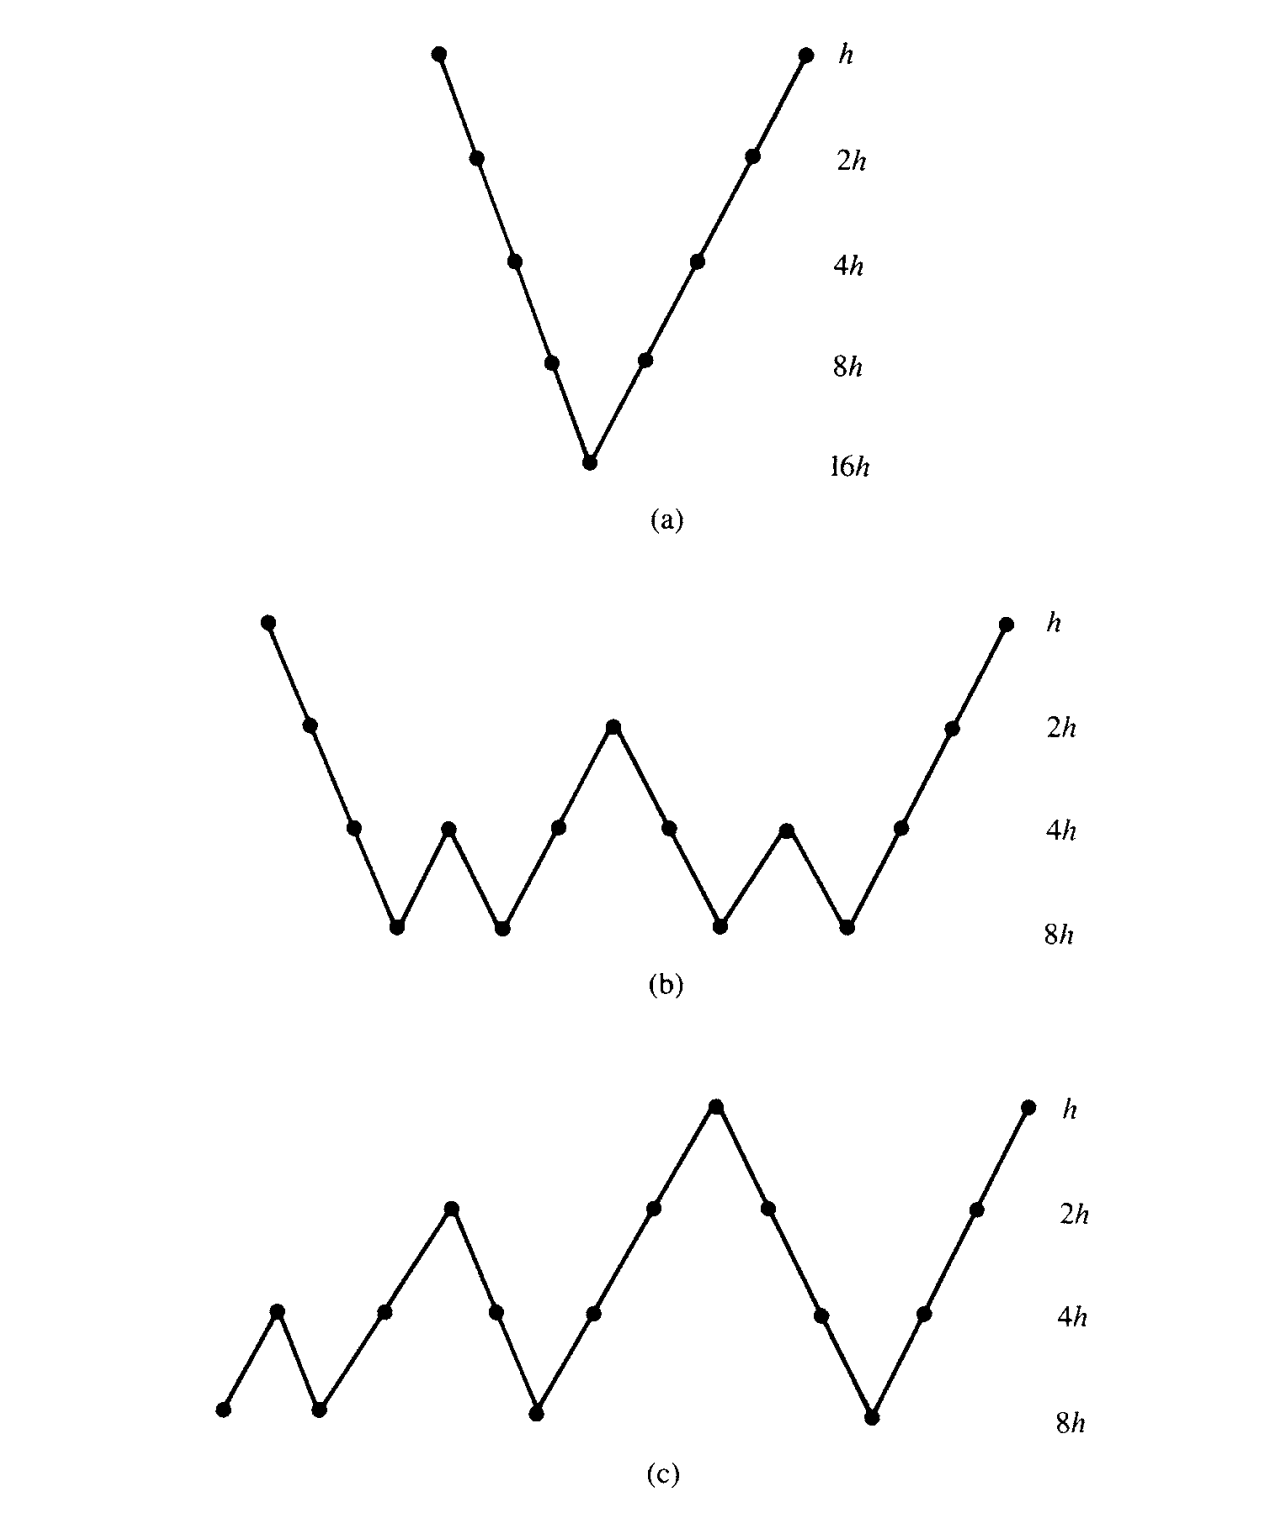
\includegraphics[width=\linewidth]{figures/multigrid_scheme.png}
    \caption{Schedule of grids for (a) V-cycle, (b) W-cycle, and (c) FMG scheme,
all on four levels. \citep{10.5555/357695}}
    \label{fig:multigrid_scheme}
\end{figure}

Earlier work in multigrid relies on the geometric structure to construct coarse problems, thus this approach is called geometric multigrid.  In problems where the computational domain is not composed of well-structured meshes, the multigrid method can be also applied via algebraic operators rather than a geometric grid.  This approach is called the algebraic multigrid. We will cover this approach in the next subsection.

\subsection{Algebraic Multigrid}
  The classical multigrid formed around the geometric structure has been generalized that the multigrid is analyzed in terms of the matrix properties \citep{mccormick1982multigrid}. This algebraic approach to theory was further extended to form the basis for much of the early development that led to the so-called Ruge-St{\"u}ben or classical algebraic multigrid (CAMG) method \citep{brandt1986algebraic,mandel1988algebraic,ruge1987algebraic}. A detailed overview of the algebraic multigrid can be found in this recent paper \citep{xu2017algebraic}. Here, we want to present it more concisely.
  We begin this subsection with the following theorem in linear algebra taken from \citep{10.5555/357695}.
\begin{theorem}[Solvability and the Fundamental Theorem of Linear
Algebra]
Suppose we have a matrix $A \in \mathbf{R}^{m\times n}$. The fundamental theorem of linear algebra states that the range (column space) of the matrix, $\mathcal{R}(A)$, is equal to the orthogonal
complement of $\mathcal{N}(A^T)$, the null space of ${A}^{T}$. Thus, spaces $\mathbf{R}^m$ and $\mathbf{R}^n$ can be
orthogonally decomposed as follows:
\begin{align}
    \mathbf{R}^m &= \mathcal{R}(A) \oplus \mathcal{N}(A^T)\\
     \mathbf{R}^n &= \mathcal{R}(A) \oplus \mathcal{N}(A)
\end{align}
For the equation $A\mathbf{u}=\mathbf{f}$ to have a solution, it is necessary that the vector $\mathbf{f}$ lie in $\mathcal{R}(A)$. Thus, an equivalent condition is that $\mathbf{f}$ be orthogonal to every vector in $\mathcal{N}(A^T)$. For the equation $A\mathbf{u}=\mathbf{f}$ to have a \textit{unique} solution, it is necessary that $\mathcal{N}(A) = \{\mathbf{0}\}$. 
Otherwise, if $\mathbf{u}$ is a solution and $\mathbf{v} \in \mathcal(A)$, then $A(\mathbf{u} + \mathbf{v}) = A\mathbf{u} + A\mathbf{v} = \mathbf{f} + \mathbf{0} = \mathbf{f}$, so the solution is not unique.
\end{theorem}
This is another point to view the coarse-grid correction scheme, and this leads to the algebraic multigrid. More theories related to this topic and the spectral picture of multigrid can be found in \citep{10.5555/357695}.

The unique aspect of the CAMG is that the coarse problem is defined on a subset of the degrees of freedom of the initial problem, thus resulting in both coarse and fine points, which leads to the term CF-based AMG. A different approach to constructing algebraic multigrid is called \textit{smoothed aggregation} (SA) AMG, where collections of degrees-of-freedom define a coarse degree-of-freedom \citep{vanvek1996algebraic}. Together, CF and SA form the basis of AMG and led to several developments that extend AMG to a wider class of problems and architectures.

AMG does not depend on the geometry of the problem and discretization schemes, and due to this generalizability, it has been implemented in different forms in many software libraries. The original CAMG algorithm and its variants are available as \texttt{amg1r5} and \texttt{amg1r6} \citep{ruge1987algebraic}. A parallel implementation of the CF-based AMG can be found in the BoomerAMG package in the Hypre library \citep{yang2002boomeramg}. The Trilinos package includes \texttt{ML} as a parallel SA-based AMG solver \citep{gee2006ml}.
PETSc adopts a geometric algebraic multigrid (GAMG) based on smoothed aggregation \citep{petsc-web-page}.
Finally, PyAMG includes a number of AMG variants for testings, and Cusp distributes with a standard SA implementation for use on a GPU \citep{dalton2014cusp,bell2022pyamg}. 

\subsection{The Multigrid Method Within the SBP-SAT Scheme}
Since the SBP-SAT scheme is a framework for discretization to form a linear system, it is compatible with the multigrid method and can be accelerated using this technique. The key challenge from simply applying the common prolongation and restriction operators with the Galerkin condition \autoref{galerkin-condition} is that the summation-by-parts property would not be preserved for the coarse grid operators. In order to accurately represent the coarse-grid correction problem for the SBP-SAT scheme, a more suitable class of interpolation operators needs to be proposed. Many works have been done to address this issue \citep{RUGGIU2018216}.

To overcome this issue, consider defining the restriction operator as 
\begin{equation}
    I_r = H_2^{-1}I_p^TH_1
    \label{eqn:interpolation_sbp}
\end{equation}
which was first introduced in \citep{RUGGIU2018216}. This involves the coarse grid SBP norm $H_2$ and is obtained by enforcing that two scalar products
\begin{align}
    (\phi_1,\psi_1)_{H_1} &= (\phi_1H_1\psi_1) \\
     (\phi_2,\psi_2)_{H_2} &= (\phi_2H_2\psi_2)
\end{align}
are equal for $\phi_1 = I_p\phi_2$ and $\psi_2 = I_r \psi_1$. $\phi$ and $\psi$ correspond to the $\boldsymbol{u}$ and $\boldsymbol{v}$ in the previous section on iterative solvers. We use these new notations to avoid confusion with the $\mathbf{u}$ used in the previous subsection on the multigrid method. As a result, the interpolation operators $I_r$ and $I_p$ are adjoints to each other with respect to the SBP-based scalar products defined in \citep{hackbusch2013multi}.
\begin{align}
    (I_p,\xi_2,\xi_1)_{H_1} = (\xi_2,I_r\xi_1)_{H_2}
    \label{eqn:adjoint}
\end{align}

by using \autoref{eqn:interpolation_sbp}, it is possible to build pairs of consistent and accurate prolongation and restriction operators. The following definition of the SBP-preserving interpolation operators was given in \citep{RUGGIU2018216}, where the operators were used to couple SBP-SAT formulations on grids with different mesh sizes with numerical stability.



\begin{definition}
  Let the row-vectors $\mathbf{x}_1^k$ and $\mathbf{x}_2^k$ be the projections of the monomial $x^k$ onto equidistant 1-D grids corresponding to a fine and coarse grid, respectively. $I_r$ and $I_p$ are then called 2$q$-th order accurate SBP-preserving interpolation operators if $I_r\mathbf{x}_1^k - \mathbf{x}_2^k$ and $I_p\mathbf{x}_2^k - \mathbf{x}_1^k$ vanish for $k = 0, ...,2q-1$ in the interior and for $k=0,...,q-1$ at the boundaries.
\end{definition}


The sum of the orders of the prolongation and restriction operators should be at least equal to the order of the differential equation. As a consequence, the use of high-order interpolation is not required here to solve the linear system with the multigrid method. However, high-order grid transfer operators can be used in combination with high-order discretization \citep{sundar2015comparison}. 

SBP-preserving interpolation operators with minimal bandwidth are given in Appendix A. The restriction operator $I_r$, which differs from the conventional one at boundary nodes, is shown in \autoref{fig:sbp_restriction}.


\begin{figure}
    \centering
    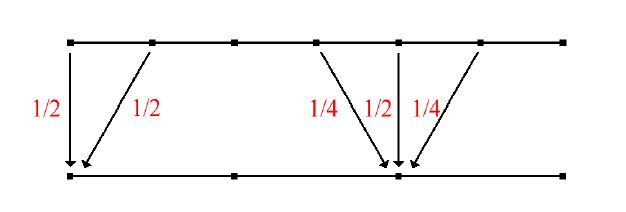
\includegraphics{figures/sbp_restriction.png}
    \centering
    \caption{The 2nd-order SBP-preserving restriction operator $I_r$ \citep{RUGGIU2018216}}
    \label{fig:sbp_restriction}
\end{figure}




\subsubsection{SBP-preserving interpolation applied to the first derivative}
Using Galerkin condition \autoref{galerkin-condition} and SBP-preserving operators, we can construct the linear system with the multigrid method. We first consider the first derivative fine-grid SBP operator $D_{1,1}$ and its coarse-grid counterpart $D_{1,2}$ constructed as follow
\begin{equation}
    D_{1,2} = I_r D_{1,1} I_p
\end{equation}
We now show that $D_{1,2}$ preserves SBP property in such ways. To start with, we rewrite the left-hand side of the following SBP property

\begin{equation}
    (\phi,D_1\psi)_H = \phi_N\psi_N - \phi_0\psi_0 - (D_1\phi,\psi)_H
\end{equation}
with the adjoint relation \autoref{eqn:adjoint} as follows
% \begin{align}
%     (\phi_2,D_{1,2}\psi_2)_{H_2} &= (\phi_2,I_r(D_{1,1}I_p\phi_2))_{H_2} \nonumber\\&= (I_p\phi_2,D_{1,1}(I_p\psi_2))_{H_1}
% \end{align}

\begin{equation}
    (\phi_2,D_{1,2}\psi_2)_{H_2} = (\phi_2,I_r(D_{1,1}I_p\phi_2))_{H_2} = (I_p\phi_2,D_{1,1}(I_p\psi_2))_{H_1}
\end{equation}

Next, the SBP property for the finite-grid operator $D_1$ leads to
\begin{equation}
     (\phi_2,D_{1,2}\psi_2)_{H_2} = (I_p,\phi_2)_N(I_p,\psi_2)_N - (I_p,\phi_2)_0(I_p,\psi_2)_0 - (D_{1,1}(I_p\phi_2),I_p\psi_2)_{H_1}
     \label{eqn:sbp_multigrid}
\end{equation}

Both grids are conforming to the domain boundaries, and the prolongation onto the boundary nodes of the fine grid is exact. Furthermore, by applying \autoref{eqn:adjoint} to the right-hand side of \autoref{eqn:sbp_multigrid}, we obtain 
\begin{equation}
    (\phi_2,D_{1,2}\psi_2)_{H_2} = \phi_{2,N/2}\psi_{2,N/2} - \phi_{2,0}\psi_{2,0} - (D_{1,2}\phi_{2},\psi_{2})_{H_2}
\end{equation}
And we've shown that the coarse grid operator $D_{1,2}$ constructed in a such way preserves the SBP property. Also, the coarse grid first derivative SBP operator $D_{1,2}$ retains the order of accuracy of the original scheme at the interior nodes if 2$q$th order SBP-preserving interpolations are used. The proof can be found in \citep{RUGGIU2018216}.

\subsubsection{SBP-preserving interpolation applied to the second derivative}
The SBP-preserving interpolation can also be applied to the second derivative operator. Similar to the proof for the first derivative operator, we can prove that the coarse grid operator constructed in such ways preserves the SBP property.

The interpolation operators in \autoref{eqn:interpolation_sbp} lead to a coarse-grid second derivative operator $D_{2,2}$ which preserves the summation-by-parts property in \autoref{eqn:2d_sbp}. We can show that by rewriting the left hand side of the \autoref{eqn:2d_sbp} for $D_{2,2}$ and the two coarse-grid functions $\phi_2$ and $\psi_2$ by using \autoref{eqn:adjoint}.
\begin{equation}
    (\phi_2,D_{2,2}\psi_2)_{H_2} = (\phi_2,I_r,D_{2,1}I_p\psi_2)_{H_2} = (I_p\phi_2,D_{2,1}I_p\psi_2)_{H_1}
\end{equation}
By applying the SBP property \autoref{eqn:2d_sbp} for the fine-grid second derivative $D_{2,1}$, we have
\begin{equation}
    (\phi_2,D_{2,2}\psi_2)_{H_2} = (I_p\phi_2)_N(SI_p\psi_2)_N - (I_p\phi_2)_0(SI_p\psi_2)_0 - (SI_p\phi_2)^TA(SI_p\psi_2)_{H_2}
\end{equation}

Both grids are conforming to domain boundaries, implying that $(I_p\phi_2)_i = \phi_{2,i/2}$ and $(SI_p\psi_2) = (S\phi_2)_{i/2}$ for $i\in\{0,N\}$. Thus 
\begin{equation}
     (\phi_2,D_{2,2}\psi_2)_{H_2} = \phi_{2,N/2}(S\phi_2)_{N/2} - \phi_{2,0}(S\phi_2)_0 - (SI_p\phi_2)^TA(SI_p\psi_2)_{H_2}
\end{equation}
where $S$ is equivalent to $\boldsymbol{d}_0^T$ which approximates the first derivative at the boundaries as discussed in the previous section on the SBP-SAT methods.

Additional proofs or propositions to SBP-preserving interpolations can also be found in  \citep{RUGGIU2018216}. Furthermore, several model problems have been tested with multigrid iteration schemes using these SBP-preserving interpolations. These problems include a Poisson equation, the anisotropic elliptic problem, and the advection-diffusion problem. Numerical experiments show that the SBP-preserving interpolation improves convergence properties of the multigrid scheme for SBP-SAT discretizations regardless of the order of the discretization and smoother chosen. Moreover, the excellent performance in combination with the smoother SOR, clearly indicates that multigrid algorithms with SBP-preserving interpolation can be designed to get fast convergence. The paper mainly covers the steady model problem to compare the effect of different grid transfer operators. For time-dependent problems, the effectiveness of multigrid algorithms with these SBP-preserving interpolations needs to be tested \citep{RUGGIU2018216}.


\subsection{Multigrid Preconditioned Conjugate Gradient}
In the previous sections, we introduce the classical iterative solvers and Krylov subspace methods as a solver. Moreover, we show that the classical iterative solvers can be used in the multigrid method as smoothers. And we provide the basic knowledge on preconditioners for iterative methods. However, using multigrid as a preconditioner for the conjugate gradient is an alternative approach motivated by engineering problems.

The multigrid method is a very effective iterative method for the mechanical analysis of heterogeneous material samples in \citep{hafner2006mesoscale}. However, the increase in the ratio of Young's moduli between matrix material and inclusion leads to a significantly worse condition number of the system, which slows the solution process. This could be also the result of the worse material representation on coarse grids. For a similar problem, Poisson's equation with large coefficient jumps or differences of grid spacing in coordinate transformation, the worse condition number will also lead to the slow solving process with the iterative methods mentioned above. As Poisson's equation is the key challenge in earthquake cycle simulation, an effective approach to solving linear systems with worse condition numbers is worth exploring. It has been shown that the multigrid preconditioned conjugate gradient method has a superior convergence rate over the multigrid method as a solver \citep{tatebe1993multigrid}. This approach is less dependent on the considered problem.


 The conditions of the multigrid preconditioners are examined in \citep{tatebe1993multigrid}. According to \citep{wesseling2004introduction}, the multigrid method will potentially provide a valid preconditioner if the smoother is symmetric. For a derivation of the preconditioned conjugate gradient method, we would introduce a matrix $\boldsymbol{L}$ which satisfies $\boldsymbol{M}^{-1} = \boldsymbol{L}^T\boldsymbol{L}$ as shown in \citep{wesseling2004introduction} (Our notation $\boldsymbol{M}$ is equivalent to $\boldsymbol{H}$ in the paper). The \autoref{eqn:preconditioned-system}  improves the convergence if the condition number of the preconditioned matrix $\boldsymbol{M}^{-1}\boldsymbol{A}$ is lower than that of the original matrix $\boldsymbol{A}$, which can be determined from the analysis of eigenvalues as presented in \citep{hackbusch2013iterative}. If the preconditioning matrix is exactly $\boldsymbol{M}^{-1} = \boldsymbol{A}^{-1}$, the after one iteration step, the exact solution $\boldsymbol{u}$ is found. An ideal preconditioning matrix $\boldsymbol{M}^{-1}$ should be a reasonably close approximation of $\boldsymbol{A}^{-1}$. With respect to the initial search direction, the vector $\boldsymbol{p}^0 = \boldsymbol{M}^{-1}\boldsymbol{r}^0$ would correspond to the error $-\boldsymbol{e}^0$, if $\boldsymbol{M}^{-1} = \boldsymbol{A}^{-1}$. An adequate matrix $\boldsymbol{M}^{-1}$ leads to an improved initial search direction $\boldsymbol{p}^0$. Therefore, the preconditioned conjugate gradient method applies the following start conditions
\begin{equation}
    \boldsymbol{r}^0 = \boldsymbol{f} - \boldsymbol{A}\boldsymbol{u}^0; \quad \tilde{\boldsymbol{r}}^0 = \boldsymbol{p}^0 = \boldsymbol{A}^{-1}\boldsymbol{r}^0
\end{equation}
The following equations give a preconditioned conjugate gradient method adapted from \citep{tatebe1993multigrid} in the notation of the conjugate gradient method in \autoref{section:krylov_subspace}.
% \begin{align}
%     \lambda_k &= \frac{\tilde{\boldsymbol{r}}^{k^T} \boldsymbol{r}^k}{}
% \end{align}
\begin{align}
    \lambda_k &= \frac{\tilde{\boldsymbol{r}}^{k^T}\boldsymbol{r}^k}{{\boldsymbol{p}^k}^T\boldsymbol{A}\boldsymbol{p}^k} \\
    \boldsymbol{u}^{k+1} &= \boldsymbol{u}^k + \lambda_k\boldsymbol{p}^k \\
    \boldsymbol{r}^{k+1} &= \boldsymbol{r}^k - \lambda_k\boldsymbol{A}\boldsymbol{p}^k \\
    \tilde{\boldsymbol{r}}^{k+1} &= \boldsymbol{M}^{-1} \boldsymbol{r}^{k+1} \label{step:pcg}\\
    \boldsymbol{p}^{k+1} &= \tilde{\boldsymbol{r}}^{k+1} + \frac{\tilde{\boldsymbol{r}}^{{k+1}^T}\boldsymbol{r}^{k+1}}{\tilde{\boldsymbol{r}}^{k^T}\boldsymbol{r}^k} \boldsymbol{p}^k % something wrong with the spacing here
\end{align}

In each iteration step, preconditioning only takes place in \autoref{step:pcg} and generates a new vector $\tilde{\boldsymbol{r}}^{k+1}$. The preconditioning matrix $\boldsymbol{M}^{-1}$ does not need to be explicitly built. The operation defined in \autoref{step:pcg} can be replaced by a multigrid cycle that solves a linear system with $\boldsymbol{r}^{k+1}$ being the right hand side, and the solution is then assigned to $\tilde{\boldsymbol{r}}^{k+1}$. The preconditioned conjugate gradient method preserves a system of conjugate directions, while each increment is optimized for each improved search direction based on the multigrid method. Therefore, this optimization leads to considerably improved increments, if the stiffness of the coarse meshes is generally overestimated.

\section{Geometric multigrid for SBP-SAT method}
%%%%%% Algorithms
To apply multigrid efficiently for the SBP-SAT method on GPUs, we need to develop a new geometric multigrid formulation that does not require using algebraic coarsening or Galerkin's condition.

Matrix-free iterative methods enable the solution to larger problems compared to a direct solve that requires storing a matrix factorization.  However, the convergence of CG depends predominantly on the condition number and quality of the initial guess. The condition number can be reduced through preconditioning techniques, but the preconditioning matrix $\mathbf{M}$ has to be SPD and fixed, and although it need not be explicitly assembled nor inverted, good preconditioners should satisfy $\mathbf{M} \approx \mathbf{A}^{-1}$. 


To our knowledge, preconditioning has not been explored for CG methods applied to SBP-SAT discretizations. 
% Existing work using multigrid as a solver for problems with SBP-SAT methods focused on using SBP-preserving interpolation operators with the Galerkin coarsening to build the coarse grid operators 
Existing work using multigrid as a solver for problems with SBP-SAT methods focused on using SBP-preserving interpolation operators with the Galerkin coarsening to build the coarse grid operators \citep{RUGGIU2018216}. Here the standard interpolation operators were modified for boundary points to preserve the SBP property \citep{RUGGIU2018216}. However, although Galerkin coarsening or other algebraic multigrid methods produce coarse grid operators automatically (and therefore can be seen as a ``plug-in" solver for any linear system \citep{stuben2001review}), defining these matrix-free coarse grid operators in this fashion requires writing a different kernel for every grid level, as well as more memory for data storage \citep{brandt2006guide}. 
Moreover, it also increases overhead in pre-compiling matrix-free kernels for different $N$s due to the just-in-time (JIT) compiling mechanism in Julia. Therefore, to fully utilize the efficiency of our matrix-free methods, as well as to reduce complexity in and number of kernels needed, developing geometric multigrid preconditioned CG (denoted MGCG) for the SBP-SAT method becomes the key focus of our work. 

Three key ingredients define multigrid methods, namely, interpolation operators (prolongation and restriction), smoothers, and (if used) a direct solve on a coarse grid.  In this work we adopt the second-order SBP-preserving prolongation/restriction operators from \citep{RUGGIU2018216}, which maintain accuracy at domain boundaries and correctly transfer residual vectors to the coarser grids. The 2D restriction operator is given by

\begin{equation}
    \boldsymbol{I}_{h}^{2h} = \boldsymbol{H}_{2h}^{-1} \left(\boldsymbol{I}_{2h}^h\right)^T\boldsymbol{H}_h
\end{equation}
%
where $\boldsymbol{H}_{h}$ and $\boldsymbol{H}_{2h}$ denote $\boldsymbol{H} \otimes \boldsymbol{H}$ with grid spacing $h$ and $2h$, respectively. The 2D prolongation operator $\boldsymbol{I}_{2h}^h$ is defined by $\boldsymbol{I}_{2h}^h = I_{2h}^h \otimes I_{2h}^h$, where $I_{2h}^h$ is the standard 1D prolongation operator \citep{10.5555/357695}, see Appendix A in \citep{RUGGIU2018216}.

One feature that differentiates our problem formulation from those in \citep{RUGGIU2018216} is that our matrix in SBP-SAT methods is rendered SPD only after the multiplication of \eqref{eqn: D2} on the left by $\left(\boldsymbol{H} \otimes \boldsymbol{H} \right)$, which introduces additional grid information when calculating the associated residual vector. To properly transfer this grid information we found improved performance when further modifying the restriction operator to account for grid spacing. This is achieved by excluding the $\left(\boldsymbol{H} \otimes \boldsymbol{H} \right)$ term when computing the residual on the fine grid, then restricting using $\boldsymbol{I}_r$, and then re-introducing the grid spacing on the coarse grid. This process requires ``applying" the inverse: Given that $\left(\boldsymbol{H} \otimes \boldsymbol{H} \right)$ is a sparse diagonal matrix (thus its inverse is the diagonal matrix of reciprocal values), GPU kernels for the multiplication of this matrix and its inverse can be easily implemented in a matrix-free manner. The pseudo-code for the geometric multigrid method is given in Algorithm \autoref{alg:mg-modified}.





\begin{algorithm*}
    \caption{$(k+1)$-level MG for $\boldsymbol{A}_h \boldsymbol{u}_h = \boldsymbol{f}_h$, with smoothing $S_{h_k}^{\nu}$ applied $\nu$ times. SBP-preserving restriction and interpolation operators are applied. Grid coarsening ($k \to k+1$) is done through successive doubling of grid spacing until reaching the coarsest grid. The multigrid cycle can be performed $N_{maxiter}$ times. $\boldsymbol{r}$ represents the residual, and $\boldsymbol{v}$ represents the solution to the residual equation used during the correction step. This algorithm is adapted from \citep{liu2023multigrid}.}\label{alg:mg-modified}
    \algrenewcommand\algorithmicprocedure{\textbf{function}}
    \begin{algorithmic}
    \Procedure{MG}{$\boldsymbol{f}_{h_k}$, $\boldsymbol{A}_{h_k}$, $\boldsymbol{u}_{h_k}^{(0)}$, $k$, $N_{maxiter}$}
    \For {$n = 0, 1, 2, \dots, N_{maxiter}$} 
                
        \State $\boldsymbol{u}_{h_k}^{(n)}$ $\xleftarrow[]{S_{h_k}^{\nu_1}}$ $\boldsymbol{u}_{h_k}^{(n)}$ \Comment{Pre-smoothing $\nu_1$ times}
        \State  $\boldsymbol{r}_{h_k}^{(n)} = \boldsymbol{f}_{h_k}^{(n)} - \boldsymbol{A}_{h_k}^{(n)} \boldsymbol{u}_{h_k}^{(n)}$ \Comment{Calculating residual}
        \State  $\tilde{\boldsymbol{r}}_{h_{k}} =  (\boldsymbol{H}_k \otimes \boldsymbol{H}_k)^{-1} \boldsymbol{r}_{h_k}^{(n)}$  \Comment{Removing grid info}
    
        \State     $\boldsymbol{r}_{h_{k+1}} = (\boldsymbol{H}_{k+1} \otimes \boldsymbol{H}_{k+1}) \boldsymbol{I}_{h_{k}}^{h_{k+1}} \tilde{\boldsymbol{r}}_{h_{k}}$ \Comment{Restriction}
        \If{$k + 1 = k_\text{max}$}
        \State $\boldsymbol{v}_{h_{k+1}}^{(n)}$ $\xleftarrow[]{S_{h_{k+1}}^{\nu_2}}$ $\boldsymbol{0}_{h_{k+1}}^{}$ 
                    \Comment{Smoothing on coarsest grid}
        \Else
        \State $\boldsymbol{v}_{h_{k+1}}^{(n)}$ = MG({$\boldsymbol{r}_{h_{k+1}}$, $\boldsymbol{A}_{h_{k+1}}$, $\boldsymbol{0}_{h_{k+1}}^{}$, $k + 1$, $1$})
        \State       \Comment{Recursive definition of MG}   
        \EndIf
        \State  $\boldsymbol{v}_{k}^{n} = \boldsymbol{I}_{h_{k+1}}^{h_k} \boldsymbol{v}_{k+1}^{(n)}$
                 \Comment{Interpolation}
        \State $\boldsymbol{u}_{k}^{(n+1)} = \boldsymbol{u}_{k}^{(n)} + \boldsymbol{v}_{k}^{n}$ \Comment{Correction}
        \State   $\boldsymbol{u}_{k}^{(n+1)} \xleftarrow[]{S_{h_k}^{\nu_3}}$ $\boldsymbol{u}_{h_k}^{(n+1)}$ \Comment{Post-smoothing $\nu_3$ times}
    \EndFor
    \EndProcedure
    % \Require
    \end{algorithmic}
\end{algorithm*}






Many types of smoothers for multigrid methods can be explored for best performance.  In this work we choose the Richardson iteration given by $\mathbf{x}_{k+1} = \mathbf{x}_k + \omega (\mathbf{b} - \mathbf{A}\mathbf{x}_k)$
because it can be easily implemented with our existing matrix-free kernel. Here $\omega$ is chosen to satisfy the convergence criteria and its optimal value depends on the eigenvalues of $\boldsymbol{A}$ as $\omega_{opt} = \frac{2}{\lambda_{max} + \lambda_{min}}$, where $\lambda_{max}$ and $\lambda_{min}$ are the largest and smallest eigenvalues of $\boldsymbol{A}$ respectively.
We use Arpack.jl, which is a Julia wrapper of ARPACK that uses the Implicitly Restarted Arnoldi Method to calculate eigenvalues for sparse matrices.
For small $N$, we can compute $\lambda_{max}$ and $\lambda_{min}$ directly, but for large $N$ values, these become computationally intractable. We use interpolation to approximate values for $\lambda_{max}$ and $\lambda_{min}$ for $N \geq 32$ based on observation of eigenvalues for $N \leq 32$, namely,
%
\begin{align*}
    \lambda_{min, 2N} &= \lambda_{min, N} / 4, \\
    \lambda_{max, 2N} &= \lambda_{max, N} + 0.6 * (\lambda_{max, N} - \lambda_{max, N/2}),
\end{align*}
where $\lambda_{min, N}$ represents the minimal eigenvalue of a linear system formed for our 2D problem with $N+1$ grid points in each direction and $\lambda_{max, N}$ is the corresponding maximum value.
In practice, these interpolated eigenvalues provide a relatively tight lower and upper bound for the real eigenvalues and appear to be sufficient according to our performance results.
Alternative smoothers could be considered, such as Jacobi iteration or SSOR, but these require the decomposition of the linear system and the development of additional GPU kernels. 
We did test these smoothers in experiments using the matrix-explicit formulation and found that they perform at similar levels to the Richardson iteration when multigrid is used as a preconditioner. We found that the total number of iterations required by MGCG is largely determined by the number of grid levels and smoothing steps and is less impacted by the choice of smoother itself. 
%
\begin{figure}[t]
    \centering
    %\includegraphics[width=\textwidth]{sparsity_patter_A.png}
    %  \includegraphics[width=0.8\textwidth]{mgcg_richardson.pdf}
    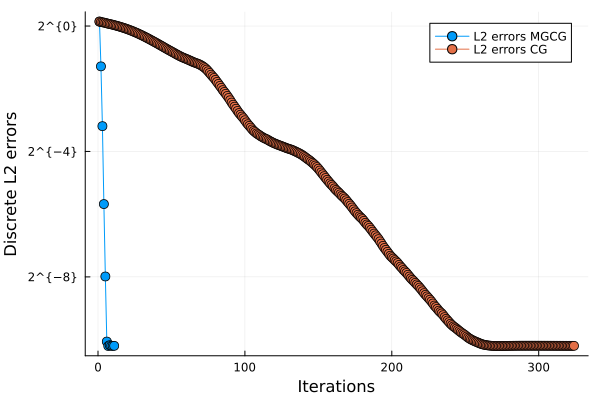
\includegraphics[width=\linewidth]{figures/64_L2_errors.png}
    \caption{Log of error (difference from a direct solve) versus iteration count for multigrid preconditioned conjugate gradient (MGCG), shown in blue circles, using 5 steps of pre- and post-Richardson smoothing for every level versus unpreconditioned conjugate gradient (CG), shown in orange circles, for $N = 2^5$.}
    \label{fig:mgcg_conv}
\end{figure}
%
%



Multigrid methods have many tunable parameters. For this initial study, we implemented MGCG with 5 Richardson pre- and  post-smoothing steps on every level with a single V-cycle (i.e. taking $\nu_1 = \nu_2 = \nu_3 = 5$ and $N_{maxiter} = 1$ in Algorithm 1), including on the coarsest grid (5 grid points in each direction). This avoids using a direct solve on the coarse grid which would require conversion between CPU arrays and GPU arrays.
All operations in this MGCG algorithm can be implemented in a matrix-free manner in a way that does not require storing matrix $\boldsymbol{A}$ on any grid level.  
% We compare our matrix-free MGCG (denoted MF-MGCG) algorithm against the standard, non-preconditioned CG algorithm implemented with cuSPARSE. 

% The results are given Table \ref{tab:mgcg}. Our matrix-free implementation beats SpMV consistently whether or not we use preconditioning. We also see that the MGCG algorithms beat the direct solve consistently for both matrix-free and SpMV implementations.  As $N$ doubles, the number of iteration steps for MGCG stays at the same level $\sim$10.

% The MGCG requires a relatively constant number of iterations to converge as $N$ is doubled, but CG requires 2$\times$ more iteration steps when $N$ is doubled, presumably due to an increase in condition number.
To show the drastically different behaviors, we plot the discrete $\mathit{L}^2$-error against iteration counts for $N = 32$ for CG and MGCG in \autoref{fig:mgcg_conv}.
MGCG converges after only $\sim$5 iterations. Additional iterations are coming from the additional discrete $\mathit{L}^2$-error requirement in the stopping criteria.
Since the complexity of each CG iteration step is $\mathcal{O}(N^2)$, as $N$ doubles the total time increases by a factor of 4 for MGCG versus 8 for CG. 
% The number of degrees of freedom quadruples when $N$ is doubled. As a result, the total throughput in degrees of freedom remains at the same level of magnitude for MGCG methods, but the CG and direct solve see memory throughput reduced by roughly 2$\times$ when $N$ doubles, see Table \ref{tab:DOF}. Memory throughput drops for $N=2^{13}$ as compared to $N=2^{12}$ for the MF-MGCG due to the increased iteration count. 
% This is because of the $\mathit{L}^2$-error used in the stopping criterion. For MGCG using only the residual stopping criterion, the peak performance for $N=2^{13}$ is above $70$ MDoF/s.
In this section we present a new formulation multigrid preconditioned conjugate gradient that can be implemented matrix-free with a Richardson smoother in order to solve 2D, variable coefficient elliptic problems discretized with an SBP-SAT method. 

%We show that matrix-free kernels outperform the cuSPARSE SpMV kernels from NVIDIA in both runtime and memory usage.
% The MGCG algorithm achieves nearly constant iteration steps to converge for various problem sizes, reducing iteration steps by up to $4000\times$ and total runtime by up to $600\times$.



\section{Parallel Processing and HPC}
\subsection{Parallel Implementation of Iterative Methods}
\label{section:parallel}
The iterative methods are ideal for their low memory requirements, and this becomes extremely important as the simulations in many fields of study have moved towards three-dimensional models. Another appealing part of iterative methods is that they are far easier to implement in parallel than sparse direct methods because they only require a small set of computational kernels. However, iterative methods are usually slower than direct methods, especially for smaller problems, requiring suitable preconditioning techniques for accelerated convergence. The parallel aspect of preconditioners also becomes very important naturally.

This subsection gives a short overview of various parallel architectures as well as different types of operations in iterative methods that can be parallelized.

% \subsubsection{Different Parallel Architectures}
There are currently three leading architectures of parallel models around which modern parallel computers are designed. These are
\begin{itemize}
    \item The shared-memory model
    \item Single-instruction-multiple-data (SIMD)
    \item The distributed memory message passing model
\end{itemize}

\subsubsection{Shared memory computers}
A shared memory computer has processors connected to a large global memory, and the address space is the same for all processors. Data stored in a large global memory is readily accessible to any processor. There are two possible implementations of shared memory machines: 
\begin{itemize}
    \item bus-based architectures
    \item switch-based architectures
\end{itemize}

\begin{figure}[h!]
    \centering
    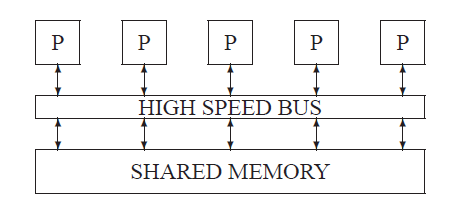
\includegraphics[width=\linewidth]{figures/bus-based-shared-memory.png}
    \caption{A bus-based shared memory computer \cite{doi:10.1137/1.9780898718003}}
    \label{fig:bus-shared}
\end{figure}

\begin{figure}[h!]
    \centering
    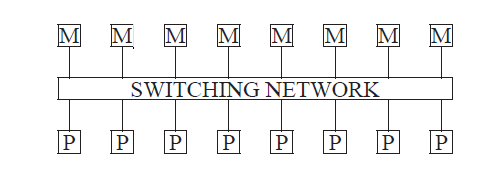
\includegraphics[width=\linewidth]{figures/switch-based-shared-memory.png}
    \caption{A switch-based shared memory machine \cite{doi:10.1137/1.9780898718003}}
    \label{fig:switch-shared}
\end{figure}

These two architectures are illustrated in \autoref{fig:bus-shared} and \autoref{fig:switch-shared}. So far, the bus-based model has been used more often. Buses are the backbone for communication between the different units of most computers, and usually have higher bandwidth for data I/O. The main reason why the bus-based model is more common is that the hardware involved in such implementation is simpler \cite{adeli1987parallel}. However, memory conflicts as well as the necessity to maintain data coherence can lead to worse performance. Moreover, shared memory computers can not take advantage of data locality in problems such as solving PDEs. Some machines can even have logically shared but physically distributed memory.

\subsubsection{Distributed Memory Architectures}
The \textit{distributed memory} model can refer to distributed memory SIMD architecture or distributed memory with \textit{memory passing} interface. A typical distributed memory system consists of a large number of identical processors and each processor has its own memory. These processors are interconnected in a regular topology. This can be shown with \autoref{fig:distributed-memory}. In these diagrams, each processor unit can be viewed as a complete processor with its one memory, CPU, I/O subsystems, control unit, etc. These processors are linked to a number of ``neighboring'' processors. In the ``message passing'' model, no global synchronizations are performed of the parallel tasks. Instead, computations are \textit{data driven} because each processor performs a given task only when the operands it requires become available. The programmer needs to explicitly instruct data exchanges between different processors.

\begin{figure}
    \centering
    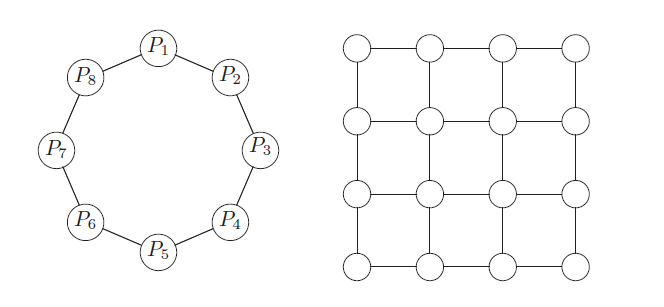
\includegraphics[width=\linewidth]{figures/distributed-memory.png}
    \caption{An eight-processing ring (left) and 4 $\times$ 4 multiprocessor mesh (right) \cite{doi:10.1137/1.9780898718003}}
    \label{fig:distributed-memory}
\end{figure}



In the SIMD model, a different approach is used. A host processor stores the program and each slave processor holds different data. The host broadcasts instructions to each processor to execute them simultaneously. One advantage of this approach is that there is no need for large memories in each node to store the main program since the same instructions are broadcast to each processor.

Unlike the shared-memory model, distributed memory computers can easily exploit the data locality of data to reduce communication costs. Modern GPUs are designed with the SIMD model (more accelerately Single-instruction-multiple-threads, SIMT) \cite{owens2008gpu}, and clusters with multiple CPUs are connected using a message passing interface (MPI) \cite{barker2015message}.


\subsection{Key Operations in Parallel Implementation}
\subsubsection{Types of Operations}

We use the preconditioned Conjugate Gradient to demonstrate the typical operations involved that can be parallelized. The PCG algorithm consists of the following types of operations:
\begin{itemize}
    \item Preconditioner setup
    \item Matrix-vector multiplications
    \item Vector update
    \item Dot Product
    \item Preconditioning operations
\end{itemize}

Matrix-vector multiplications, vector updates, and dot products are common operations in so-called Basic Linear Algebra Subprograms (BLAS) that can be easily parallelized and have been well studied and implemented for dense matrices\cite{10.1145/77626.79170,chtchelkanova1997parallel,freeman1992parallel}. In terms of the computational costs, the vector update and dot product are much lower compared to the matrix-vector multiplication, which can still be carried out very quickly on the latest GPUs. The tricky part or the bottleneck for both memory and the runtime lies in the first step of preconditioner setup and the last step of preconditioning operations. We will discuss these two key operations in the next subsection. For now, let's focus on the Matrix-vector multiplication that has much higher computational costs than the vector update and the dot product.

\subsubsection{Sparse Matrix-vector Products}
The linear system coming from the discretization in the finite difference method is often sparse, which allows us to store them efficiently and use sparse matrix-vector products (SpMVs) for efficient computation. Different formats for storing sparse matrices can be found in \cite{doi:10.1137/1.9780898718003}. Compressed Sparse Row (CSR) sparse matrix format is one of the earliest sparse formats developed. It is ideal for parallelization since the data from each row can be handled independently. The SpMV algorithm for CSR format as well as the demonstration of the storage scheme of the CSR format is shown in \autoref{fig:csr}

\begin{figure}[h!]
    \centering
    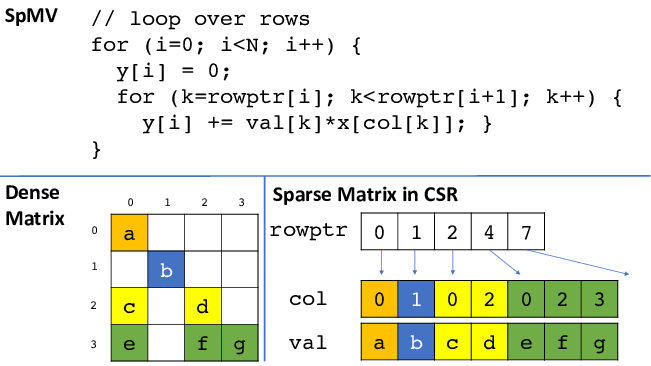
\includegraphics[width=\linewidth]{figures/Compressed-Sparse-Row-CSR-sparse-matrix-format-The-val-array-stores-the-nonzeros-by.png}
    \caption{The \texttt{val} array stores the nonzeros by packing each row in contiguous locations. The \texttt{rowptr} array points to the start of each row in the \texttt{val} array. The \texttt{col} array is parallel to \texttt{val} and maps each nonzero to the corresponding column.\cite{mohammadi2018sparse}}
    \label{fig:csr}
\end{figure}



A summary of different sparse matrix formats in the following table as well as a detailed performance comparison of these different formats can be found in \cite{stanimirovic2009performance}.
\begin{table}[h!]
\begin{tabular}{llll}
\toprule
Short & Name  & Short & Name            \\
\midrule
DNS        & Dense & Ell        & Ell-pack ItPack \\
BND           & Linpack Banded      &  DIA            & Diagonal                \\
COO           & Coordinate      & BSR           &  Block Sparse Row               \\
CSR           & Compressed Sparse Row      &    SSK        &    Symmetric Skyline             \\
CSC           &  Compressed Sparse column      & BSR           &  Nonsymmetric Skyline               \\
MSR           & Modified CSR       &    JAD        &    Jagged Diagonal             \\
    LIL       & Linked List      &            &                \\
\bottomrule
\end{tabular}
\caption{A summary of different sparse matrix formats and their short names}
\end{table}
There are also recent work on developing new sparse matrix formats for optimal performance for different use cases \cite{smailbegovic2005sparse,dongarraxz1994sparse} or implementing SpMV algorithms on parallel architectures \cite{bell2009,yan2014yaspmv,li2014performance}. Using the right sparse matrix formats and implementing them on suitable architectures can reduce the time spent on these SpMV calculations significantly, which makes iterative methods run faster. Another way to accelerate these iterative methods is to use the preconditioners that we mentioned before. A parallel implementation of these preconditioners becomes more challenging because of the complex arithmetic operations compared to the SpMV or other BLAS operations. We will focus on the parallel preconditioning technique in the next subsection.




\subsection{Parallel Preconditioning}

\subsubsection{Parallelism in Solving Linear Systems}
Each preconditioned step from the previous subsection requires the solution of a linear system of equations of the form $Mz = y$. We consider traditional preconditioners such as ILU or SOR or SSOR, in which a solution with $M$ is the result of solving triangular systems. Since these preconditioners are commonly used, it's important to explore their efficient parallel implementations for the iterative methods to be parallel. These preconditioners are mostly implemented on shared memory parameters. The distributed memory computers would use different strategies. These preconditioners require some sort of factorization, and the parallelism is done by sweeping through the lower triangular matrix or upper triangular matrix. Typical parallelism can be seen using a forward sweep. 

It's typical for solving a lower triangular system that the solution is overwritten onto the right-hand side. So there is only one array $u$ needed for both the solution and the right-hand side. The forward sweep for solving lower triangular systems with coefficients $A(i,j)$ and right-hand-side $b$ is defined as follows:
% \begin{algorithm}
% \caption{Sparse Forward Elimination}\label{alg:two}ß
%     \For{$i = 2 \dots n$}{
%         \For{ \text{all $j$ that $A(i,j)$ is nonzero}}{
%             $u(i)$ $\gets$ $u(i) - A(i,j) * u(j)$    \\
%         }
%     }
% \end{algorithm}
\begin{algorithm}
\caption{Sparse Forward Elimination}\label{alg:two}
\begin{algorithmic}[1]
    \For{$i \gets 2$ to $n$}
        \For{each $j$ such that $A(i,j) \neq 0$}
            \State $u(i) \gets u(i) - A(i,j) \times u(j)$
        \EndFor
    \EndFor
\end{algorithmic}
\end{algorithm}

Here $A(i,j)$ refers to the element in the sparse matrix. The different sparse matrix formats will have different implementations of locating this element, so the inner for loop will be implemented differently and the $A(i,j)$ will be replaced by different indexing code in different sparse matrix formats.

\subsubsection{Parallel preconditioners}
Several techniques can be for parallel implementations of the preconditioners. They can be summarized into three types of techniques.
The simplest approach is to use a Jacobi or block Jacobi approach. In this case, a Jacobi preconditioner may be consist of a diagonal or a block-diagonal of $A$
To improve the performance, these preconditioners can be accelerated by polynomial iterations. For example, the second level of preconditioning is called \textit{polynomial preconditioning}.

A different strategy is to enhance parallelism by using graph algorithms, such as graph-coloring techniques. The gist of this approach is that all unknowns associated with the same color can be determined simultaneously in the forward or backward sweeps.

The third strategy uses generalizations of "partitioning" techniques which can be also called "domain decomposition" approaches.

We will give a brief overview of these methods in this part.

Overlapping block-Jacobi preconditioning is a parallel preconditioner similar to the general block-Jacobi approach with overlapping blocks as shown in \autoref{fig:overlap-block-jacobi}. Enlarging a system of algebraic equations by including duplicate copies of several rows, leads to an efficient iterative scheme on a multiprocessor MIMD array \cite{WAIT1988325}. 
\begin{figure}[h!]
    \centering
    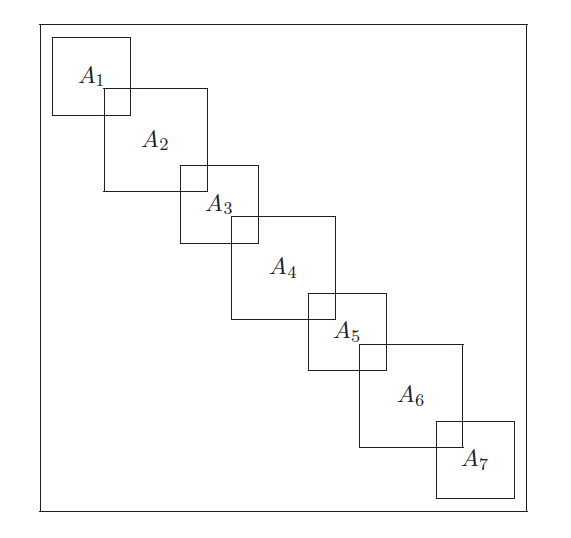
\includegraphics[width=\linewidth]{figures/block-jacobi.png}
    \caption{The block-Jacobi matrix with overlapping blocks \cite{doi:10.1137/1.9780898718003}}
    \label{fig:overlap-block-jacobi}
\end{figure}


Polynomial preconditioners are another family of parallel preconditioners. In polynomial preconditioners, the matrix $\boldsymbol{M}$ is defined by $\boldsymbol{M^{-1} = s(A)}$, where $\boldsymbol{s}$ is a polynomial, typically of low degree. Thus the original system can be preconditioned by 
\begin{equation}
    \boldsymbol{s(A)Au = s(A)f}
\end{equation}
Note that the $\boldsymbol{s(A)}$ and $\boldsymbol{A}$ commute, and as a result, the preconditioned matrix is the same for left or right preconditioning. In addition, the matrix $\boldsymbol{s(A)}$ or $\boldsymbol{As(A)}$ does not need to be formed explicitly in matrix form, which allows the use of matrix-free methods.
This approach was initially motivated by the good performance of matrix-vector operations on vector computers. It has now become more popular on iterative methods for GPU computing because of the similar SIMD architecture. 
There are several ways to construct polynomials in this method.
% The simplest polynomial $s$ is the polynomial of the Neumann series expansion
% \begin{equation}
%     I + N + N^2 + \cdots + N^s
% \end{equation}
% In which
% \begin{equation}
%     N = I - \omega A
% \end{equation}
% $\omega$ is called the scaling parameter. The series above comes from expanding the inverse of $\omega A$ using the splitting
% \begin{equation}
%     \omega A = I - (I - \omega A)
% \end{equation}
% This approach can be generalized using the splitting of the form
% \begin{equation}
%     \omega A = D - (D - \omega A)
% \end{equation}
% where $D$ can be a diagonal of A, or a block diagonal of A.
% Then
% \begin{align}
%     (\omega A)^{-1} &= [D(I - (I - \omega D^{-1}A))]^{-1} \nonumber \\
%     &= [I - (I - \omega D^{-1}A)]^{-1}D^{-1}
% \end{align}
% Thus, setting
% \begin{equation}
%     N = I - \omega D^{-1}A
% \end{equation}
% results in the approximate $s$-term expansion
% \begin{equation}
%     (\omega A)^{-1} \approx M^{-1} = [I + N + \cdots + N^s]D^{-1}
% \end{equation}
% Since $D^{-1}A = \omega^{-1}[I - N]$, note that

% \begin{align}
%     M^{-1}A & = [I + N + \cdots + N^s]D^{-1}A \nonumber \\
%     &= \frac{1}{\omega}[I + N + \cdots + N^2](I - N) \nonumber \\
%     &= \frac{1}{\omega}(I - N^{s+1})
% \end{align}


% The matrix operation with the preconditioned matrix can be difficult numerically for large $s$. If the original matrix is SPD, then even though $M^{-1}A$ is not symmetric, it is self-adjoint with respect to the $D-inner$ product.

% The polynomial $s$ can be selected to be optimal in some sense, and this leads to the Chebyshev polynomials. The criterion used to make the preconditioned matrix $s(A)A$ as close as possible to the identity matrix in some sense. For example, the spectrum of the preconditioned matrix can be made as close as possible to that of the identity. We denote the spectrum of $A$ by $\sigma(A)$, and by $\mathbb{P}_k$ the space of polynomials of degree not exceeding $k$. We need to solve the following problem
% \begin{align}
%     &\text{Find} s \in \mathbb{P}_k \text{ which minimizes:} \\
%     &\max\limits_{\lambda \in \sigma(A)}|1 - \lambda s(\lambda)| 
% \end{align}
% This problem involves all eigenvalues of $A$, and is hard to solve than the original problem. It can be replaced by the following problem
% \begin{align}
%     &\text{Find} s \in \mathbb{P}_k \text{ which minimizes:} \\
%     &\max\limits_{\lambda \in E}|1 - \lambda s(\lambda)| 
% \end{align}
% which is obtained by replacing the set $\sigma(A)$ by some continuous set $E$ that encloses it. Thus, a rough idea of the spectrum of matrix $A$ is needed. If $A$ is SPD, then $E$ can be taken as an interval $[\alpha,\beta]$ containing the eigenvalues of $A$.
% A variation of the approximation theorem says for any real scalar $\gamma$ such that $\gamma \leq \alpha$
% the minimum
% \begin{equation}
%     \min\limits_{p \in \mathbb{P}_k,p(\gamma)=1} \max\limits_{t \in [\alpha,\beta]}|p(t)|
% \end{equation}
% is reached for the shifted and scaled Chebyshev polynomial of the first kind
% \begin{equation}
%     \hat{C}_k(t) = \frac{C_k(1+2\frac{\alpha - t}{\beta - \alpha})}{C_k (1+2\frac{\alpha - \gamma}{\beta - \alpha})}
% \end{equation}
% When $\gamma = 0$, this gives the polynomial 
% \begin{equation}
%     T_k(t) = \frac{1}{\sigma_k}C_k(\frac{\beta + \alpha - 2t}{\beta - \alpha}) \text{ with } \sigma_k = C_k(\frac{\beta+\alpha}{\beta - \alpha})
% \end{equation}
One of the most commonly studied approach is called the Chebyshev iteration that can be found in \cite{doi:10.1137/1.9780898718003}. One nice feature of the Chebyshev iteration is that it does not require inner products, and this is very attractive for parallel implementation as it does not require reductions.

Other polynomials include least-squares polynomials. A comparison of Chebyshev polynomials and least-square polynomials can be found in \cite{ashby1992comparison}. So far, Chebyshev polynomials have been the most popular for parallel implementation, especially in the matrix-free setting where the assembly of the matrix can be very expensive.
Multicolor preconditioners are similar to ILU preconditioners in the sense that the construction and factorization of the matrices are required. Methods like these can be done in parallel, but they are not suitable for GPUs.

\subsection{GPU architecture and CUDA}
Given the increasing importance and popularity of GPUs in modern supercomputers, this subsection is dedicated to GPU architecture. As NVIDIA GPUs are mostly used in the industry for scientific computing and machine learning, the GPU programming model will be focused on CUDA (Compute Unified Device Architecture) toolkit.

A GPU is built as a scalable array of multithreaded \textit{Streaming Multiprocessors} (SMs), each of which consists of multiple \textit{Scalar Processor} (SP) cores. To manage hundreds or thousands of threads, the multiprocessors employ a \textit{Single Instruction Multiple Threads} (SIMT) model with each thread mapped into one SP core and executing independently with its own instruction address and register state.
Threads are organized in \textit{warps}. A warp is defined as a group of 32 threads of consecutive thread IDs. More detailed information on optimizing memory access patterns can be found in \cite{wilt2013cuda}.

The NVIDIA GPU platform has various memory architectures. The types of memory can be classified as follows:
\begin{itemize}
    \item off-chip global memory
    \item off-chip local memory
    \item on-chip shared memory
    \item read-only cached off-chip constant memory and texture memory
    \item registers
\end{itemize}

The effective bandwidth of each type of memory depends significantly on the access pattern. Global memory is relatively large but has a much higher latency. Using the right access pattern such as memory coalescing and avoiding bank conflicts will help achieve good memory bandwidth.


GPUs were initially designed for graphics-related calculations such as image rendering. General-purpose GPU programming on NVIDIA GPUs is supported by the NVIDIA CUDA toolkit. CUDA programs use similar syntax to C++. The main code on the host (CPU) would invoke a \textit{kernel grid} that runs on the device (GPU). The same parallel kernel is executed by many threads. These threads are organized into thread blocks. Blocks and threads are the logical division of the GPU and are mapped to the actual SMs. Thread blocks are split into warps scheduled by SIMT units. All threads in the same block share the same shared memory and can be synchronized by a barrier. Threads in a warp execute one common instruction at a time. This is referred as warp-level synchronization \cite{wilt2013cuda}. It's most efficient when 32 threads of a warp follow the same execution path. Branch divergence in which threads within the same warp are executing different instructions often causes worse performance/

CUDA is only a lower-level tool for direct kernel programming. Libraries built on top of CUDA allow users to directly use code and kernels written for different tasks without manually programming and optimizing kernels themselves. Existing common CUDA libraries that supports GPU SpMV operation include CUDPP (CUDA Data Parallel Primitives)\cite{harris2007cudpp}, NVIDIA Cusp library \cite{dalton2014cusp}, and the IBM SpMV library \cite{baskaran2009optimizing}. In these packages, different formats of sparse matrices are studied for producing high-performance SpMV kernels on GPUs. These include the compressed sparse row (CSR) format, the coordinate format (COO), the diagonal (DIA) format, the ELLPACK (ELL) format., and a hybrid (ELL/COO) format. There are other recent sparse matrix formats specifically designed for GPU computing, but we will not go into detail to cover each of them.

For dense linear algebra computations, the MAGMA (Matrix Algebra for GPU and Multicore Architectures) project hybrid multicore-multi-GPU system aims to develop a dense linear algebra similar to LAPACK\cite{agullo2009numerical}. Since our numerical methods for PDEs would generate a sparse linear system, we did not explore this library in this paper.





%--- Chapter 3 ----------------------------------------------------------------%
\chapter{Scientific Computing Libraries and languages}
\section{PETSc}

PETSc, which stands for Portable, Extensible Toolkit for Scientific Computation, is a software library developed primarily by Argonne National Library to facilitate the development of high-performance parallel numerical code written in C/C++, Fortran and Python.
It provides a wide range of functionality for solving linear and nonlinear algebraic equations, ordinary and partial differential equations, and also optimization problems (provided by TAO) on parallel computing architectures.
In addition, PETSc includes support for managing parallel PDE discretizations including parallel matrix and vector assembly routines.

Key features of PETSc includes:
\begin{itemize}
    \item Parallelism: PETSc is designed for parallel computing, especially distributed-memory parallel computing architectures. It is intended to run efficiently on parallel computing systems where multiple processors or nodes communicate over the network via a message passing interface (MPI).
    These architectures include clusters, supercomputers, and other HPC platforms.
    \item Modularity and Extensibility: PETSc is highly modular and extensible, allowing users to combine different numerical techniques and algorithms to solve complex problems efficiently.
    It provides a flexible framework for implementing new algorithms and incorporating external libraries. It mainly contains the following objects
    \begin{itemize}
        \item Algebraic objects 
            \begin{itemize}
                \item Vectors (Vec) containers for simulation solutions, right-hand sides of linear systems
                \item Matrices (Mat) containers for Jacobians and operators that define linear systems
            \end{itemize}
        \item Solvers
            \begin{itemize}
                \item Linear solvers based on preconditioners (PC) and Krylov subspace methods (KSP)
                \item Nonlinear solvers (SNES) that use data-structure-neutral implementations of Newton-like methods
                \item Time integrators (TS) for ODE/PDE, explicit, implicit, IMEX
                \item Optimization (TAO) with equality and inequality constraints, first and second order Newton methods
                \item Eigenvalue/Eigenvectors (SLEPc) and related algorithms
            \end{itemize}
    \end{itemize}
    \item Efficiency and Performance: PETSc is optimized for performance, with algorithms and data structures designed to minimize memory usage and maximize computational efficiency. It supports parallel matrix and vector operations as well as efficient iterative solvers and preconditioners via the objects mentioned previously 
    \item Flexibility: PETSc supports a wide range of numerical methods and algorithms and has built-in discretization tools. It provides interfaces for solving problems in various scientific and engineering disciplines, including computational fluid dynamics (CFD), solid mechanics, etc with documented examples and tutorials for researchers.
    \item PETSc is portable across different computing platforms and operating systems, including UNIX/Linux, macOS, and Windows. It provides a consistent interface and functionalities across different architectures, making it easy to develop and deploy simulation code across multiple platforms.
\end{itemize}
\section{AmgX}

AmgX is a proprietary software library developed by NVIDIA to accelerate the solution of large-scale linear systems arising from finite element and finite volume discretizations typically found in computational fluid dynamics (CFD) and computational mechanics simulations on NVIDIA GPUs.
AmgX stands for Algebraic Multigrid Accelerated.
It provides wrappers to work with other libraries like PETSc and programming languages like Julia.

Key features of AMGX include:
\begin{itemize}
    \item Preconditioning: AmgX offers a variety of advanced preconditioning techniques, including algebraic multigrid (AMG), smoothed aggregation and hybrid methods to accelerate the convergence of iterative solvers for sparse linear systems.
    These preconditioners are designed for and tested in real-world engineering problems in collaboration with companies like ANSYS, a provider of leading CFD software Fluent.
    \item Parallelism: AmgX is optimized for NVIDIA GPUs and provides support for OpenMP to allow acceleration via heterogeneous computing and MPI to run large simulations across multiple GPUs and clusters.
    \item Flexibility and Customization: AmgX offers a flexible and extensible framework for configuring and customizing the solver algorithms via JSON files. 
\end{itemize}
The limitation of AmgX is due to its link with NVIDIA. It can not run on GPUs from other vendors, such as AMD and Intel. Some of the latest exascale supercomputers are built with CPUs and GPUs from AMD and Intel.
\section{HYPRE}
HYPRE is a software library of high performance numerical algorithms including preconditioners and solvers for large, sparse linear systems of equations on massively parallel computers \cite{Falgout2006TheDA}. 
The HPYRE library was created to provide users with advanced parallel preconditioners. It features parallel multigrid solvers for both structured and unstructured grid problems.
These solvers are called from application code via HYPRE's conceptual linear system interfaces \cite{10.5555/1125403.1125423}, which allow a variety of natural problem descriptions.

Key features of HYPRE include:
\begin{itemize}
    \item Scalable preconditioners: HYPRE contains several families of preconditioners focused on scalable solutions of very large linear systems.
    HYPRE includes "grey box" algorithms including structured multigrid that use more than just the matrix to solve certain classes of problems more efficiently.
    \item Common iterative methods: HYPRE provides several common Krylov-based iterative methods in conjunction with scalable preconditioners. 
    This includes methods for symmetric matrices such as Conjugate Gradient (CG) and nonsymmetric matrices such as GMRES.
    \item Grid-centric interfaces for complicated data structures and advanced solvers: HYPRE has improved usability from earlier generations of sparse linear solver libraries in that users do not have to learn complicated sparse matrix data structures.
    HYPRE builds these data structures for users through a variety of conceptual interfaces for different classes of users.
    These include stencil-based structured/semi-structured interfaces most suitable for finite difference methods, unstructured interfaces for finite element methods, and linear algebra based interfaces for general applications.
    Each conceptual interface provides access to several solvers without the need to manually write code for new interfaces.
    \item User options for beginners through experts: HYPRE allows users with various levels of expertise to write their code easily. The beginner users can set up runnable code with a minimal amount of effort. Expert users can take further control of the solution process through various parameters
    \item Configuration options for different platforms: HYPRE allows a simple and flexible installation on various computing platforms. Users have options to configure for different platforms during the installation.
    Additional options include debug mode which offers more info and optimized mode for better performance.
    It also allows users to change different libraries such as MPI and BLAS.
    \item Interfaces to multiple languages: HYPRE is written in C, but it also provides an interface for Fortran users.
\end{itemize}

% \section{Julia}
\section{Review of several languages for scientific computing}
\subsection{Fortran}
There are many languages designed for high performance computing.
Traditionally, Fortran has been used to write high performance numerical code.
It is short for ``Formula Translation''. As the name suggest, it is one of the oldest and most enduring programming languages in scientific computing.
Developed in the 1950s by IBM, it was designed to facilitate numerical and scientific computations, particularly for high-performance computing on mainframe computers.

Fortran was specifically designed for efficient numerical and scientific computing, with optimized operations handling mathematical operations, arrays, and complex computations \citep{10.1145/960118.808380}.
It provides a rich set of built-in functions and libraries for numerical analysis, linear algebra, differential equations, and other mathematical tasks.
It is a statically typed language, meaning that variable types are declared explicitly at compile time and do not change during runtime. This allows compilers to perform extensive type checking and optimization to generate efficient code for execution.

Fortran codes are also highly portable across different computing platforms. While early versions of Fortran (66, 77) were designed for specific hardware architectures, modern Fortran standards, such as Fortran 90, 95, 2003, 2008, and 2018 (formerly 2015) have introduced features that enhance portability and interoperability with other languages and systems. Fortran is also known for its excellent backward compatibility, with newer language standards preserving compatibility with older databases.
This allows legacy Fortran programs to continue running without modification on modern compilers and systems, ensuring long-term viability and support for existing applications, which is very important in scientific research where many simulation codes are built on top of decades of previous work.

Because of these reasons, despite its age, Fortran remains widely used in scientific and engineering computing.

\subsection{C and C\texttt{++}}
C was created in 1972 as a general-purpose programming language. C\texttt{++} was created in 1979 to enhance C language with object-oriented design \citep{10.1145/323648.323736}.
Standard template libraries were introduced in C\texttt{++} in 1990s to improve code reusability and standardization \citep{10.5555/2544010}.
Despite the historical dominance of Fortran in scientific and engineering computing, C and C\texttt{++} have gradually replaced Fortran in many scientific computing and HPC codes due to their performance, flexibility, and rich ecosystem of tools and libraries.

While Fortran continues to be used in certain domains, particularly in legacy codebases and specialized applications, the adoption of C and C\texttt{++} as the default language in many modern packages reflects the evolving needs and preferences of HPC developers for modern, versatile programming languages.

C and C\texttt{++} are known for their performance and efficiency. 
In fact, they are often used as the standard to compare the performance of various programming languages. 
This is because they provide low-level control over hardware resources and memory management, allowing programmers to write code that executes with high speed and minimal overhead. 
The performance is crucial for HPC applications, which often involve computationally extensive tasks and large-scale simulations.
Known as somewhat high-level languages, C and C\texttt{++} strike a balance between high-level abstractions and low-level control. They support multiple programming paradigms including procedural, and object-oriented.
C/C\texttt{++} can also be extended to handle parallel processing via pragma directives.
This allows the creation of modular, reusable code with encapsulation, inheritance, polymorphism, and templates.
Standard Libraries built on top of these features provide implementations of fundamental data structures, algorithms, and utilities.

In addition to their language features, C and C\texttt{++} offer support for concurrency and parallelism via low-level features like threads, mutexes, condition variables, atomic operations, and parallel algorithms.
Modern C\texttt{++} standards (such as C\texttt{++}11, C\texttt{++}17 and C\texttt{++}20) have introduced high-level features to manage asynchronous execution, parallel computation, and parallelism-aware data structures.
All these efforts further enhance the capability of C and C\texttt{++} as high performance computing languages.

As general-purpose programming languages, C and C\texttt{++} codes are highly portable across different platforms and architectures. 
The portability is essential for deploying HPC applications on diverse computing platforms, including cloud servers, clusters, and supercomputers.
C and C\texttt{++} also have excellent interoperability with other programming languages and systems. 
They can be easily integrated with libraries and tools including most common HPC languages like Fortran, Python, and CUDA.
This interoperability allows developers to leverage existing software components and take advantage of specialized and optimized libraries for specific computational tasks.
However, the impact on the performance needs to be considered carefully when interoperating C and C\texttt{++} with other languages.

\subsection{MATLAB}
MATLAB is a high-level programming language usually used in an interactive development environment (IDE) from the software with the same name \citep{doi:10.1137/1.9781611974669}.
Developed by MathWorks, it is widely used for numerical computing, data analysis, visualization, and algorithm development.
Compared to compiled languages that can generate binary executables running natively on operation systems, MATLAB requires an interpreter (usually by MATLAB) to ``translate'' the code whenever the code is run.
To avoid ambiguity, we refer to both the language and the IDE as MATLAB here.
As a proprietary language and tool, MATLAB offers limited access to the source code, and it is prohibitively expensive for people outside of academia without an educational license.
GNU Octave is used as an open source alternative to MATLAB as it is mostly compatible with MATLAB. Octave is free and lightweight, however, it often comes with the cost of worse performance.
Despite being a proprietary software, MATLAB is still often used in scientific computing, especially in academia for the following reasons:

MATLAB is easy to use because of its intuitive syntax for mathematicians and comprehensive set of built-in functions for numerical computing, including matrix manipulation, linear algebra, and optimizations. For these functions, MATLAB offers extensive examples and tutorials, making it a great choice for beginners for learning and advanced users for writing code.

MATLAB has an interactive environment with visualization tools that enable users to iterate quickly on algorithms. It offers a command-line interface that is similar to read-evaluate-print-loop (REPL) in interpreted languages like Python, and also integrates many common functionalities via UI buttons in its IDE.
Like many IDEs, MATLAB provides tools for organizing code, debugging, profiling, and version control.
More importantly, MATLAB's functionality can be extended through its proprietary and third-party toolboxes, which are collections of specialized functions and algorithms for specific domains of applications such as signal processing, control theory, and statistics.

Because of these features and accessibility via academic licenses through educational institutes, many people start numerical coding in MATLAB and continue to develop in MATLAB for research purposes. 
Although MATLAB is designed to run numerical calculations efficiently and also provides some limited support for parallel and GPU computing, it was not designed as a HPC language running on clusters, supercomputers, and cloud infrastructures. 
Researchers often use MATLAB for quick implementation and testing during the prototyping stage and then rewrite their code in HPC languages such as FORTRAN and C/C\texttt{++}. 
This raises the so-called ``two-language'' problem which inspires the development of the Julia language.

\section{Julia langauge}

Julia is a dynamically typed language for scientific computing designed with high performance in mind \citep{bezanson2017julia}.
 Julia supports general-purpose GPU computing with the package CUDA.jl. Through communications in LLVM intermediate representations with NVIDIA's compiler, it is claimed that CUDA.jl achieves the same level of performance as CUDA C according to previous research\citep{besard2018effective}.
Aimed to address the ``two-language'' problem, Julia enables implementation ease of complex mathematical algorithms while achieving high performance, an ideal match for computational scientists without expertise in low-level language-based HPC. Julia has gained attention among the HPC community, with notable examples including The Climate Machine \citep{clima}, a new Earth System model written purely in Julia that is capable of running on both CPUs and GPUs by utilizing KernelAbstractions.jl \citep{valentin_churavy_2024_10780635}, a pure Julia device abstraction similar to Raja, Kokkos, and OCCA \citep{8945721, CARTEREDWARDS20143202, Medina}. In addition, because a large body of researchers studying SBP methods use Julia in serial, e.g. \citep{Kozdon2020HybridizedSF,ranocha2021new}, our developments will enable these users to gain HPC capabilities in their code with minimal overhead.



%%--- Chapter 4 ---------------------------------------------------------------%
\chapter{Matrix-free SBP-SAT methods on GPUs}\label{chap:matrix-free}
\section{Partial Differential Equations for the Solid Earth}
\subsection{Governing equations and boundary conditions}
Static deformation of the solid Earth over the time-scales of earthquake cycles is governed by the equilibrium equation and a constitutive relationship describing the material properties.  The standard assumption is that the Earth is linear elastic, defined on a sub-domain of $\mathbb{R}^3$.  While solutions to the 3D elasticity equations are the eventual target, 2D problems are considered in this work in order to sort out implementation details with reduced computational costs.  The 2D anti-plane shear problem \citep{antiplaneshear} is particularly ubiquitous in earthquake applications, where a vertical cross-section of a 3D problem (assuming invariance in one-direction) gives rise to an elliptic equation, where only one non-zero component of the displacement vector exists and depends on two spatial variables, namely,
\begin{equation}
    -\nabla \cdot \left({\mu} \nabla u\right) = f \quad \text{ for } (x, y) \in \Omega, 
    \label{eqn: 2D}
\end{equation}
where ${\mu}(x, y)$ is the spatially-varying shear modulus, $u$ is Earth's material displacement in the $z$-direction, and $f$ comprises body forces. In order to enable complex fault geometries and topography, we assume that $\Omega$ is a curved quadrilateral in $\mathbb{R}^2$, which enables extensions to arbitrary domains partitioned into computational blocks, \citep[e.g.][]{Kozdon2020HybridizedSF}. As Figure \ref{fig:trans}(a) illustrates, the boundary can be partitioned into four curves $\partial\Omega_i, \,\, i = 1, ..., 4$, where (for example), $\partial \Omega_3$ represents Earth's surface. The shear modulus $\mu(x, y)$ can vary in order to represent heterogeneities in the crust, for example, a sedimentary basin, which is known to trap waves, extend shaking, and increase earthquake magnitudes, \citep[e.g.][]{Boue2016}. 

In this work both Dirichlet and Neumann boundary conditions are considered for generality, as each appears in earthquake problems. For example Earth's free surface manifests as a Neumann condition and slow motion of tectonic plates is usually enforced via a Dirichlet condition \citep{Erickson2014}. As proof of concept, we consider boundary conditions
\begin{subequations}\label{eqn:2Dbc}
\begin{alignat}{3}
u &= g_{1},  &&\quad \partial\Omega_1,\\ 
u&= g_{2}, &&\quad \partial\Omega_2,\\ 
{\boldsymbol{n}} \cdot \mu\nabla u&=g_{3}, &&\quad \partial\Omega_3, \\
{\boldsymbol{n}} \cdot \mu\nabla u&=g_{4}, &&\quad \partial\Omega_4,
\end{alignat}
\end{subequations}
%
\noindent where vector $\boldsymbol{n}$ is the outward pointing normal to the domain boundary and $g_i, \,\, i = 1, ..., 4$ represent boundary data.  
\subsection{Coordinate Transformation}
In order to solve \eqref{eqn: 2D}-\eqref{eqn:2Dbc} with SBP-SAT methods, the domain $\Omega$ is transformed (via a conformal mapping) to the regular, square domain $(r, s) \in \bar\Omega = -1 \leq (r, s) \leq 1$, as in Figure \ref{fig:trans}(b). The transformed equations are given by
\begin{subequations}\label{eqn:2Dvar}
\begin{alignat}{3}
-\bar\nabla \cdot \left({\bf c} \bar\nabla u\right) &= Jf,  &&\quad{\text {for } (r, s) \in \bar\Omega}, \\ 
u &= g_{1},  &&\quad \text{face 1},\\ 
u&= g_{2}, &&\quad \text{face 2},\\ 
\hat{\boldsymbol{n}}^3 \cdot {\bf c}\bar\nabla u&=S^3_J g_{3}, &&\quad \text{face 3}, \\
\hat{\boldsymbol{n}}^4 \cdot {\bf c}\bar\nabla u&=S^4_J g_{4}, &&\quad \text{face 4},
\end{alignat}
\end{subequations}
where $\bar\nabla u = \left[\frac{\partial u}{\partial r}, \,  \frac{\partial u}{\partial s}\right]^T$, face $k$  for $k = 1, ... 4$ define the domain boundaries of $\bar{\Omega}$, given in Figure \ref{fig:trans}(b). $J >0 $ is the Jacobian and  $S^{k}_J$ is the surface Jacobian on face $k$.
Vector $\hat{\boldsymbol{n}}^k$ is the outward pointing normal to the face and $2 \times 2$ matrix ${\bf c}$ is symmetric positive definite (SPD) and encodes the variable material properties $\mu(x, y)$ and the coordinate transform, see \citep{Kozdon2020HybridizedSF, Erickson2022} for more details.

\begin{figure}
    \centering
     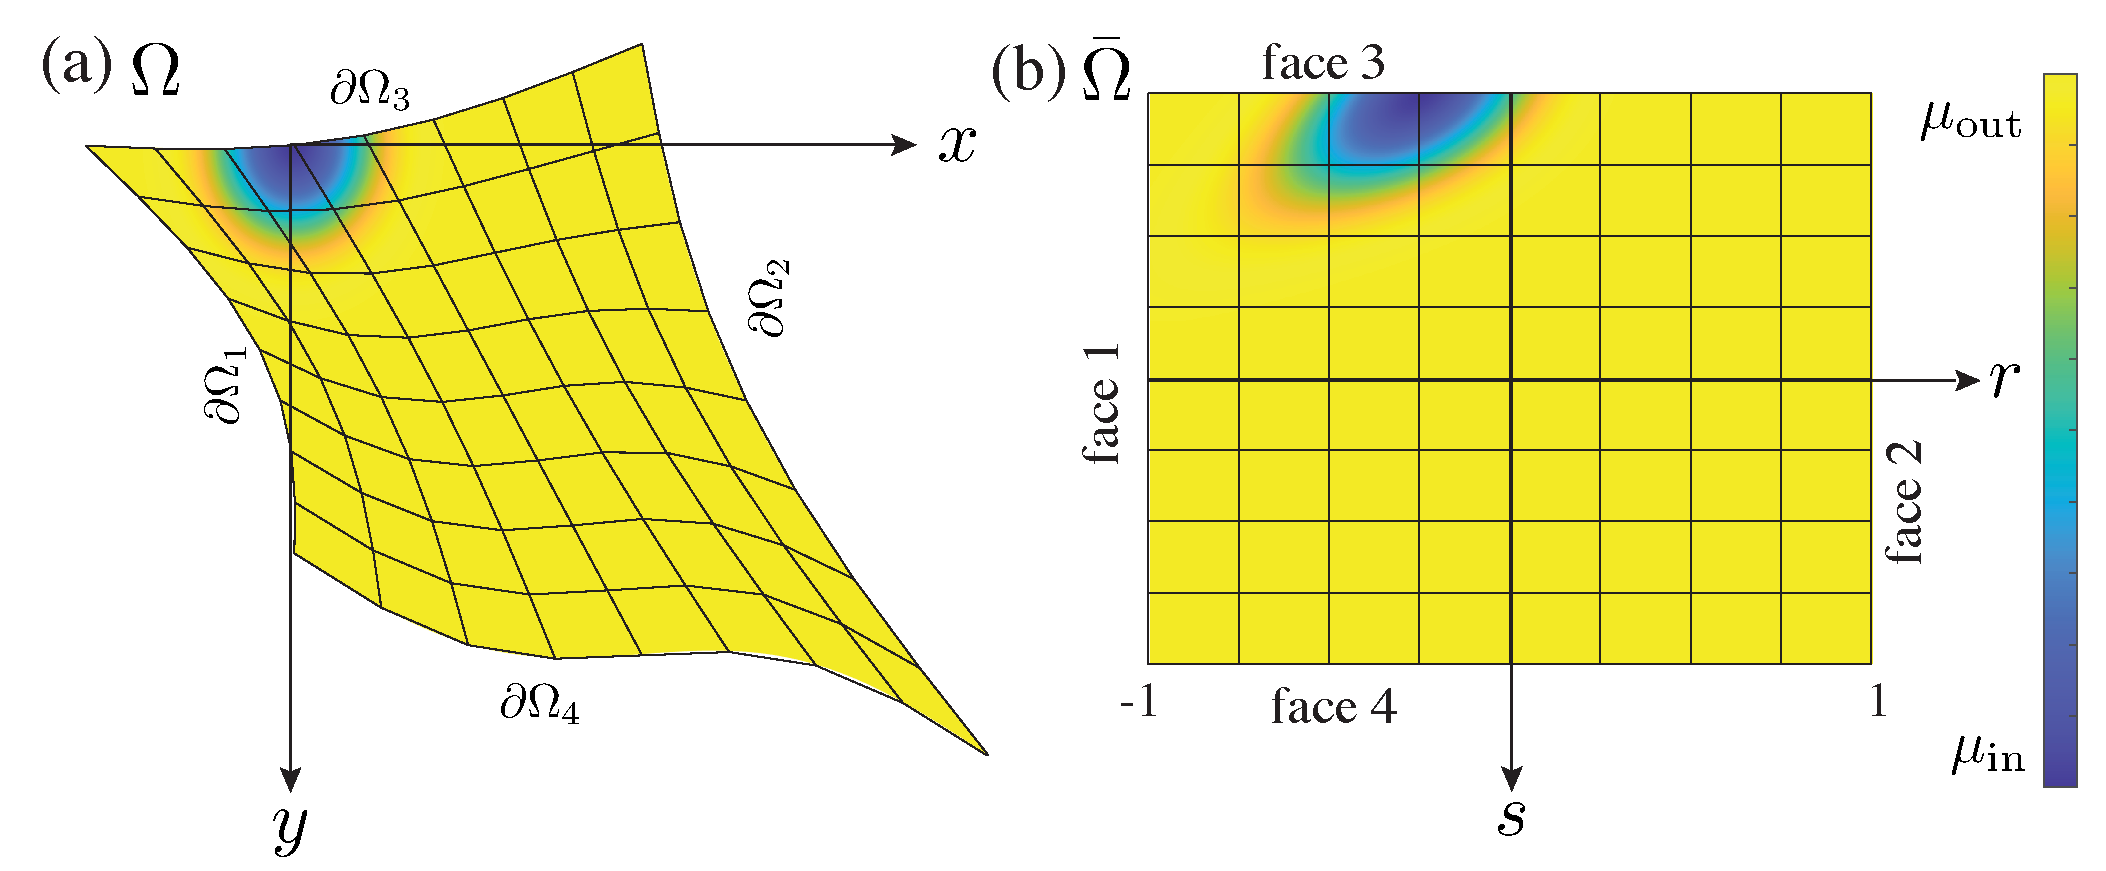
\includegraphics[width=\linewidth]{figures/grid_transformation.pdf}
    \caption{(a) Geometrically complex physical domain $\Omega$ with material stiffness that increases from $\mu_\text{in}$ within a shallow, ellipsoidal sedimentary basin, to stiffer host rock given by $\mu_\text{out}$.  (b) $\Omega$ is transformed to the regular, square domain $\bar{\Omega}$ via conformal mapping.} 
\end{figure}



\section{Problem Discretization}


\begin{figure}
    \centering
    %\includegraphics[width=\textwidth]{sparsity_patter_A.png}
     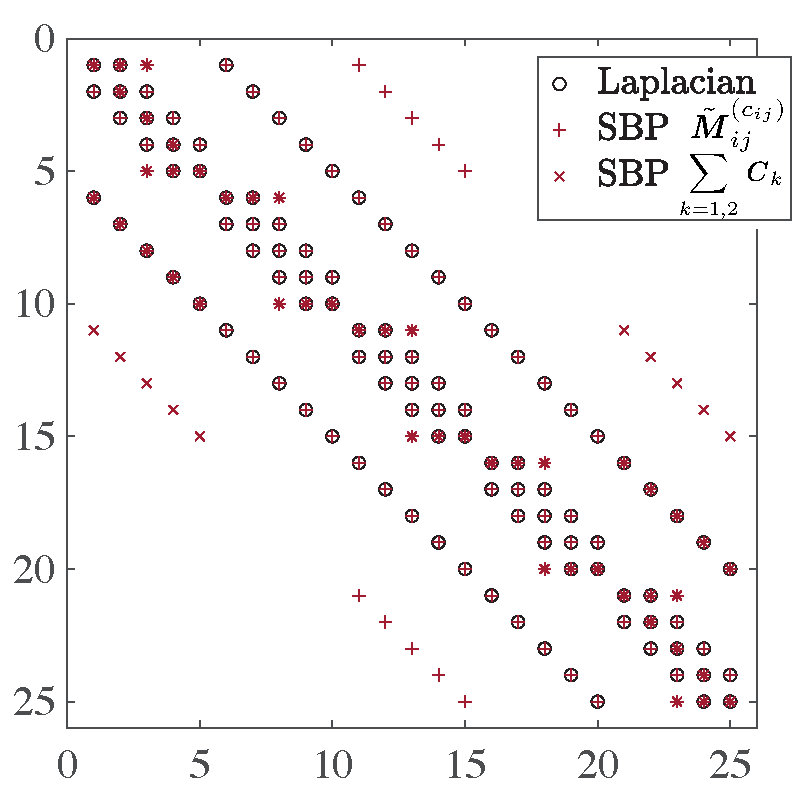
\includegraphics[width=\linewidth]{figures/iccs_spy_3.pdf}
    \caption{Sparsity pattern for matrix $\boldsymbol{A}$ with $N = 5$ grid points in each direction.  Traditional 5-point Laplacian stencil in black circles. Contributions to $\boldsymbol{A}$ are separated into contributions from the volume (red $+$) and from the boundary enforcement (red $\times$), so that contributions from both (red $\ast$) cancel any deviations from symmetry.} 
    \label{fig:sparsity_A}
\end{figure}

The SBP-SAT discretization to \eqref{eqn:2Dvar} is given by
\begin{equation}\label{eqn:2Ddiscrete}
    -\tilde{\boldsymbol{D}}_{ij}^{(c_{ij})}\boldsymbol{u} = \boldsymbol{Jf} + \sum_k \boldsymbol{p}_k
\end{equation}
where $\boldsymbol{p}_k$ are SAT vectors formed from the boundary condition on face $k$. To illustrate the structure of the SAT vectors, enforcing Dirichlet conditions on faces $k = 1, 2$ generates 

\begin{align}
\boldsymbol{p}_{k} &= \left(\boldsymbol{H} \otimes \boldsymbol{H}\right)^{-1}\left(\boldsymbol{G}_k^T  - \boldsymbol{L}_k^T \boldsymbol{H}_k {\boldsymbol \tau}_k   \right)\left(\boldsymbol{L}_k\boldsymbol{u} - \boldsymbol{g}_k\right), 
\end{align}


where matrix ${\bf G}_k = \hat{n}_i^k \boldsymbol{H}_k \boldsymbol{C}_{ij}^k \boldsymbol{B}_j^k$ computes the weighted derivative on face $k$. 
Matrix $\boldsymbol{\tau}_k$ = $\hat{n}^k_i \boldsymbol{C}^k_{ij}\hat{n}^k_j{\boldsymbol \Gamma}_k$, where ${\boldsymbol \Gamma}_k$ is the diagonal penalty matrix on face $k$ with sufficiently large components to ensure discrete stability, according to 

\begin{equation}
    {\boldsymbol \Gamma}_k \geq \frac{4}{h_\perp^k}{\bf I} + \frac{1}{h_\perp^k }{\bf P}_k,
\end{equation}

\noindent where 

\begin{equation}\label{eqn: minval}
{\bf P}_k = 
\begin{cases}
{\boldsymbol{C}}^{k}_{rr} ({\boldsymbol{C}}_{rr}^{k, min})^{-1}, \quad $k = 1, 2$,\\
{\boldsymbol{C}}^{k}_{ss} ({\boldsymbol{C}}_{ss}^{k, min})^{-1}, \quad $k = 3, 4$.
\end{cases}
\end{equation}
Here ${\boldsymbol{C}}^{k, min}$ is the minimum value of $c$ in the two points orthogonal to the boundary and $h_\perp^k$ is the grid spacing orthogonal to face $k$ \citep{Erickson2022}. 


Imposing Neumann conditions on faces $k = 3, 4$ corresponds to SAT vectors
\begin{align}
\boldsymbol{p}_{k} &= -\left(\boldsymbol{H} \otimes \boldsymbol{H}\right)^{-1}\boldsymbol{L}^T_k\left(\boldsymbol{G}_k \boldsymbol{u}  - \boldsymbol{H}_k \boldsymbol{S}_J^k \boldsymbol{g}_k\right).  
\end{align}



In order to render the linear system \eqref{eqn:2Ddiscrete} SPD, we multiply by $\left(\boldsymbol{H} \otimes \boldsymbol{H}\right)$ (the discrete equivalent of integrating over $\bar\Omega$ and discretizing the weak form). This process yields the final linear system 
\begin{equation}\label{eqn: final}
   \boldsymbol{A} \boldsymbol{u} = {\boldsymbol{b}} 
\end{equation} where
\begin{equation}\label{eqn:discrete}
\boldsymbol{A} = \tilde{\boldsymbol{M}}^{(c_{ij})}_{ij} + \sum_{k = 1, 2} \boldsymbol{C}_k,
\end{equation}
%

is SPD \citep{Erickson2022}, and matrices
\begin{equation}
    \boldsymbol{C}_k = -{\bf L}_k^T {\bf G}_k - {\bf G}_k^T {\bf L}_k + {\bf L}_k^T \boldsymbol{H}_k \boldsymbol{\tau}_k {\bf L}_k.
\end{equation}

Right-hand side vector $\boldsymbol{b}$ is given by
\begin{equation}
   {\boldsymbol{b}} = \left(\boldsymbol{H} \otimes \boldsymbol{H} \right)\left[\boldsymbol{J}\boldsymbol{f} + \sum_k \boldsymbol{K}_k \boldsymbol{g}_{k}\right]
\end{equation}
which encodes the source term and boundary data.  Here matrices $\boldsymbol{K}$ depend on boundary conditions; for those given in \eqref{eqn:2Dvar} they are
\begin{align}
    \boldsymbol{K}_1 &= \boldsymbol{L}_1^T  \boldsymbol{H}_1  {\boldsymbol\tau}_1 - \boldsymbol{G}_1^T \\
 \boldsymbol{K}_2 &= \boldsymbol{L}_2^T  \boldsymbol{H}_2  {\boldsymbol\tau}_2 - \boldsymbol{G}_2^T \\
  \boldsymbol{K}_3 &= \boldsymbol{L}_3^T \boldsymbol{H}_3\\
    \boldsymbol{K}_4 &= \boldsymbol{L}_4^T \boldsymbol{H}_4.
\end{align}
 Note that $\boldsymbol{A}$ includes contributions from both volume operators ($\tilde{\boldsymbol{M}}^{c_{ij}}_{ij}$) and from the SAT enforcement of boundary terms ($\boldsymbol{C}_k$), and differs from the traditional discrete Laplacian near all domain boundaries; see Figure \ref{fig:sparsity_A}. At Dirichlet boundaries (faces 1 and 2), $\boldsymbol{C}_k$ modifies the layer of three points normal to the face (i.e. the SAT imposition penalizes all points used in the computation of the derivative normal to the face).
\section{Matrix-free GPU kernels}
In this chapterr, we develop custom, matrix-free GPU kernels (specifically for SBP-SAT methods) for computations in the volume and boundaries, which show improved performance as compared to the native, matrix-explicit implementation while requiring only a fraction of memory. GPU-acceleration of our resulting matrix-free, preconditioned iterative scheme shows superior performance compared to state-of-the-art methods offered by NVIDIA.

Stencil computations have proven efficient in utilizing GPU resources to achieve optimal performance \citep{vizitiu2014optimized,krotkiewski2013efficient}. In this work we implement a similar GPU kernel for our 2D problem by matching each spatial node to a GPU thread, however, our work requires specialized treatment for domain boundaries. The most computationally expensive operator is the volume operator $\tilde{\boldsymbol{M}}^{c_{ij}}_{ij}$, which differs from traditional finite difference operators in that it involves derivative approximations at domain boundaries. However, the use of else statements in GPU kernels tends to lead to warp divergence and should be avoided. We construct the matrix-free action of $\boldsymbol{A}$, referred to as {\ttfamily mfA!}() based on node location. Kernel \autoref{alg:mfA-1} provides the partial pseudocode, i.e. it includes pseudocode for the $\tilde{\boldsymbol{M}}^{c_{ij}}_{ij}$ calculation; boundary condition calculations are further detailed in code block 1.  At interior nodes the action of $\tilde{\boldsymbol{M}}^{c_{ij}}_{ij}$ is defined by a single stencil (with spatially varying coefficients). The action of $\tilde{\boldsymbol{M}}^{c_{ij}}_{ij}$ on boundary nodes, however, has a different stencil depending on the face number and whether the node is at a corner of the domain. To avoid race conditions at corners (while minimizing conditional statements), only normal components of $\tilde{\boldsymbol{M}}^{c_{ij}}_{ij}$ are computed (as they correspond to the same stencil). For example on face 1 only the action of $\tilde{\boldsymbol{M}}^{c_{rr}}_{rr}$ and $\tilde{\boldsymbol{M}}^{c_{rs}}_{rs}$ are computed at the corners, see \autoref{fig:dots}. The action of the remaining components of $\tilde{\boldsymbol{M}}^{c_{ij}}_{ij}$ on the corner nodes are computed in computations associated with adjacent faces (faces 3 and 4). 

\begin{figure}
    \centering
    % \includegraphics[width=\linewidth]{speed_comparison_chart_v2.pdf}
    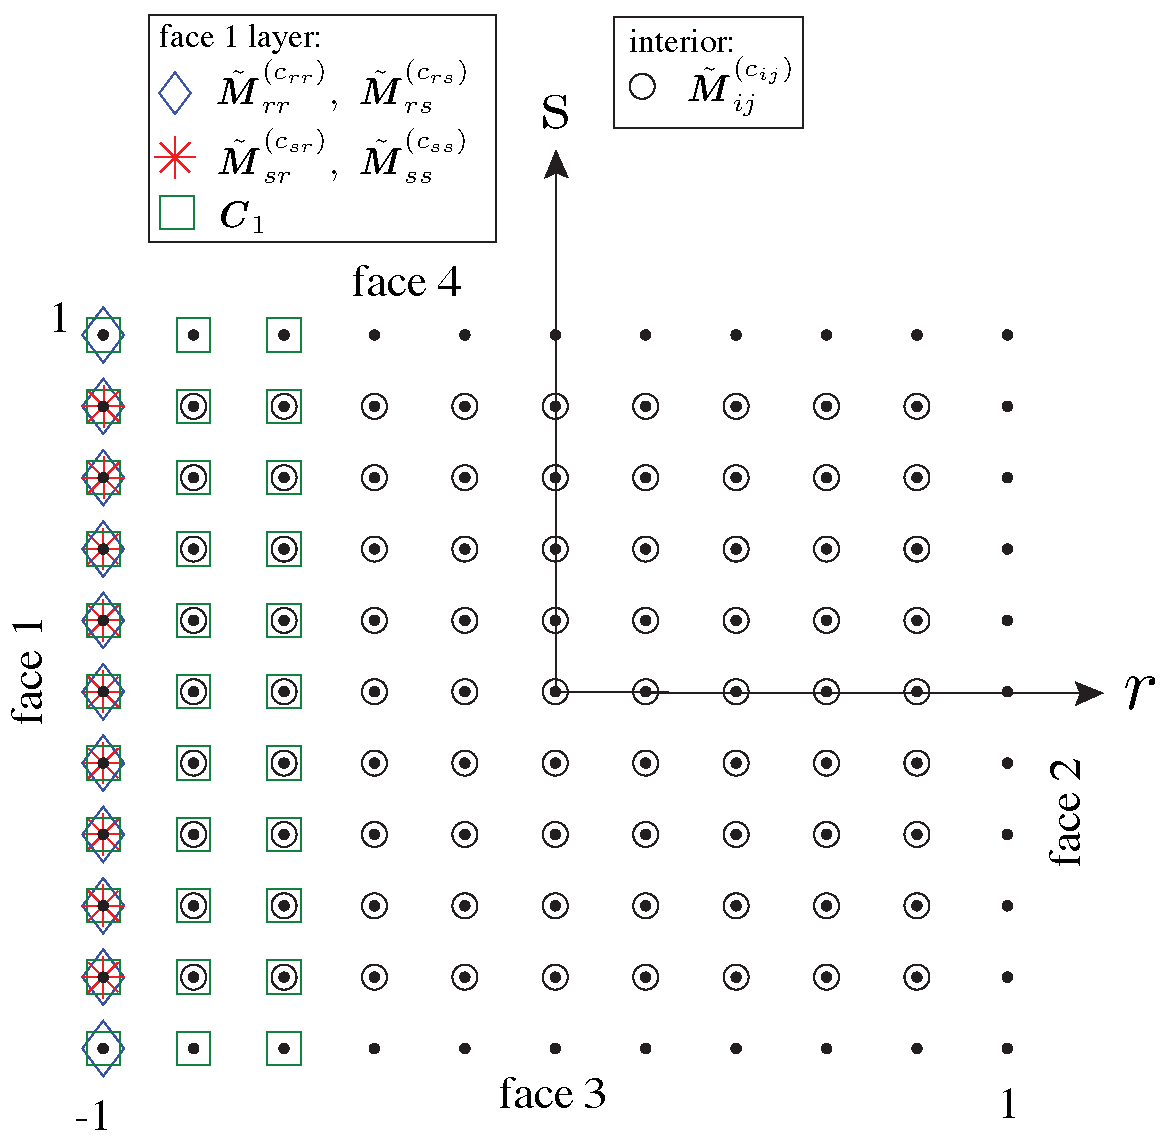
\includegraphics[width=\linewidth]{figures/dots_mod3.pdf}
    \caption{Schematic of 2D computational domain; nodes denoted with solid black dots. {\ttfamily mfA!}() modifies interior nodes, denoted with circles. For face 1, contributions to {\ttfamily mfA!}() from coordinate transformation matrices modify nodes corresponding to different shapes. Calculations by boundary operator $\boldsymbol{C}_1$ modify nodes in green squares.}
    \label{fig:dots}
\end{figure}


At boundary nodes we must also compute boundary condition operators $\boldsymbol{C}_k$, with differing stencils depending on face number and whether a node is an interior node, an interior boundary node (i.e. not a corner), or a corner node. Code block 1 provides the pseudocode for nodes on face 1; stencils are differentiated with superscripts $int, sw, nw$, corresponding to the interior boundary, northwest, and southwest corner nodes, respectively. \autoref{fig:dots} further illustrates the nodes involved in each computation: black dots correspond to nodes within the 2D domain. Black circles correspond to the interior nodes that are modified by the action of $\tilde{\boldsymbol{M}}^{c_{ij}}_{ij}$. On the western boundary (face 1), the three-node layer adjacent to face 1 is used to compute the actions of the volume and boundary operators.  Blue diamonds and red stars correspond to nodes that are modified by the different components of $\tilde{\boldsymbol{M}}^{c_{ij}}_{ij}$. Green squares correspond to the nodes that are modified by the boundary operator $\boldsymbol{C}_1$ in order to impose the Dirichlet condition (in this case a layer of three nodes normal to the face. More rows are involved for higher order $p$). 

% \setcounter{algorithm}{1}
\begin{algorithm*}
\caption{Matrix-Free GPU kernel Action of matrix-free A for interior nodes.}\label{alg:mfA-1}
\algrenewcommand\algorithmicprocedure{\textbf{function}}
\begin{algorithmic}
\Procedure{\textnormal{mfA!}}{\textnormal{odata}, \textnormal{idata}, $c_{rr}, c_{rs}, c_{ss}, h_r, h_s$}
    \State  $i, j = $get\_global\_thread\_IDs()
    \State $g = (i-1) * (N+1) + j$\Comment{compute global index}
    \If{$2 \leq i, j \leq N$} \Comment{\textnormal{interior nodes}}
        \State odata[g] = (\emph{hs}/\emph{hr})(- (0.5$c_{rr}$[$g$-1] + 0.5$c_{rr}$[$g$])\text{idata}[$g$-1] +
        \State \hspace{25mm}    + (0.5$c_{rr}$[$g$-1]  +  $c_{rr}$[$g$] - 0.5$c_{rr}$[$g$+1])\text{idata}[$g$] + 
        \State  \hspace{25mm}     - (0.5$c_{rr}$[$g$] + 0.5$c_{rr}$[$g$+1])\text{idata}[$g$+1]) + \\ \Comment{compute $M_{rr}$  stencil}\\
        \State \hspace{25mm} + 0.5$c_{rs}$[$g$-1](-0.5\text{idata}[$g$-$N$-2] + 0.5\text{idata}[$g$+$N$]) + 
        \State   \hspace{25mm} - 0.5$c_{rs}$[$g$+1](-0.5\text{idata}[$g$-$N$] + 0.5\text{idata}[$g$+$N$+1]) + \\ \Comment{compute $M_{rs}$  stencil}\\
        \State  \hspace{25mm} + 0.5$c_{rs}$[$g$-$N$-1](-0.5\text{idata}[$g$-$N$-2] + 0.5\text{idata}[$g$-$N$]) + 
        \State  \hspace{25mm} - 0.5$c_{rs}$[$g$+$N$+1](-0.5\text{idata}[$g$-$N$] + 0.5\text{idata}[$g$+$N$+2]) + \\ \Comment{compute $M_{sr}$  stencil}\\
        \State  \hspace{25mm} - (0.5$c_{ss}$[$g$-$N$-1] + 0.5$c_{ss}$[$g$])\text{idata}[$g$-$N$-1] + 
        \State  \hspace{25mm} + (0.5$c_{ss}$[$g$-$N$-1]  + $c_{ss}$[$g$] + 0.5$c_{ss}$[$g$+$N$+1])\text{idata}[$g$] - 
        \State  \hspace{25mm}     - (0.5$c_{ss}$[$g$] + 0.5$c_{ss}$[$g$+$N$+1])\text{idata}[$g$+$N$+1])) \\
        \Comment{compute $M_{ss}$  stencil}
    \EndIf
    \State  \dots \Comment{boundary nodes, e.g. Algorithm \autoref{alg:mfA-2}}
    \State \textbf{return} $nothing $ 
\EndProcedure
\end{algorithmic}
\end{algorithm*}


% \setcounter{algorithm}{2}
\begin{algorithm*}
\caption{Matrix-Free GPU kernel Action of matrix-free A for west boundary (face 1).}
\label{alg:mfA-2}
\begin{algorithmic}
\If{$2 \leq i \leq N$ \textnormal{and} $j = 1$} \Comment{\textnormal{interior west nodes}}
\State odata[$g$] = $\left(M_{rr}^{int} + M_{rs}^{int} + M_{sr}^{int} + M_{sr}^{int} + C_1^{int}\right)(\textnormal{idata})$ \\ \Comment{apply boundary $M$ and $C$ stencils}
\State  odata[$g$+1] = $C_1^{int}(\textnormal{idata})$\Comment{apply interior $C$ stencil}
\State odata[$g$+2] = $C_1^{int}(\textnormal{idata})$\Comment{apply interior $C$ stencil}
\EndIf
\If{$i = 1$ \textnormal{and} $j = 1$} \Comment{\textnormal{southwest corner node}}
\State odata[$g$] = $\left(M_{rr}^{sw} + M_{rs}^{sw} + C_1^{sw}\right)(\textnormal{idata})$ \\ \Comment{apply southwest partial $M$ and $C$  stencils}
\State  odata[$g$+1] = $C_1^{sw}(\textnormal{idata})$\Comment{apply southwest interior boundary $C$  stencil}
\State odata[$g$+2] = $C_1^{sw}(\textnormal{idata})$\Comment{apply southwest interior boundary $C$  stencil}
\EndIf
\If{$i = N+1$ \textnormal{and} $j = 1$}\Comment{\textnormal{northwest corner node}}
\State odata[$g$] = $\left(M_{rr}^{nw} + M_{rs}^{nw} + C^{nw}\right)(\textnormal{idata})$ \\ \Comment{apply northwest partial $M$ and $C$ stencils}
\State odata[$g$+1] = $C^{nw}(\textnormal{idata})$\Comment{apply northwest interior boundary $C$  stencil}
\State odata[$g$+2] = $C^{nw}(\textnormal{idata})$\Comment{apply northwest interior boundary $C$  stencil}
\EndIf
\end{algorithmic}
\end{algorithm*}



\section{Performance: Matrix-free GPU kernels}
\subsection{Performance Comparison}\label{sec: comparison}
With {\ttfamily mfA!}() we can carry out the matrix-vector product without explicitly storing the matrix. In this section, we compare its performance against the matrix-explicit cuSPARSE SpMV implementation available through CUDA.jl. We note that this is not an exhaustive comparison against all possible sparse matrix data structures.  Our goal is to establish a baseline comparison of our matrix-free implementation against the standard sparse matrix format CSR in CUDA.jl, with a focus on integration with preconditioning for improving CG performance.  





We set up our benchmark as follows: We discretize the domain $\bar{\Omega}$ in each
direction using $N+1$ grid points, varying $N$ from $2^4$ to $2^{13}$, so the
matrix $\boldsymbol{A}$ is of size $(N+1)^2 \times (N+1)^2$. \autoref{fig:A100} and \autoref{fig:V100} compare the performance of the
matrix-free implementation against the matrix-explicit SpMV provided with
cuSPARSE using the CSR format on both the A100 GPU and V100 GPU.
The performance is measured by profiling 10,000 SpMV calculations with NVIDIA Nsight Systems, and the time results shown in the figures represent the time to perform one SpMV calculation.
For problem sizes large enough for GPUs with $N$ greater than $2^{10}$, we see consistent speedup from \texttt{mfA!()} kernel with higher speedup achieved for larger problem sizes. 
On the A100 GPU, our speedup ranges from $3.0\times$ to $3.1\times$, .
On the V100 GPU, we see a similar trend, with our speedup ranging from $3.1\times$ to $3.6\times$.

The {\ttfamily mfA!}() kernel has a low arithmetic intensity of $0.28$ based on the computation of the interior points (which accounts for more than $99\%$ of the total computation and data access).
This puts the {\ttfamily mfA!}() kernel in the bandwidth-limited regime~\citep{ding2019instruction}.
If we plot this on the Roofline model, as shown in \autoref{fig:roofline} as the left red dot, we see that our kernel achieves performance that is \emph{higher} than what is possible for the given arithmetic intensity.
If we calculate the arithmetic intensity based on the assumption that the data is read from the DRAM only \emph{once} (i.e., the ideal case when the kernel only incurs compulsory cache misses), as shown in \autoref{fig:roofline} as the right red dot, we see a higher arithmetic intensity of $1.85$ and our achieved performance falls below the Roofline.
This suggests that a large portion of our data is coming from the fast memory (e.g., L1 or L2 caches), leading to performance that is better than what can be achieved if the data is only coming from the DRAM.
%That said, the {\ttfamily mfA!}() still outperforms the SpMV kernel by a large margin, showing the value of the matrix-free SBP operator. 

To confirm our hypothesis, we use NVIDIA Nsight Compute to profile our code for the problem size of N=$2^{13}$.
The profile shows that we achieved $72\%$ L1 cache hit rate and $57\%$ L2 cache hit rate, which indicates that the majority of our data is coming from the L1 and L2 caches (approximately $88\%$), and that our DRAM reads are due mostly to compulsory cache misses (i.e., when the input data is read for the first time).
This explains why our code performs better than the DRAM-bounded performance.
\autoref{fig:roofline-double-precision} shows the Roofline model generated by Nsight Compute, based on performance counter measurements of how much of the overall data is coming from different levels of the memory hierarchy.
\autoref{fig:roofline-double-precision} confirms that the majority of our data comes from the L1 cache, followed by L2 and DRAM.
It also suggests that we can further improve the performance of our $\texttt{mfA!}$() kernel by improving data reuse in the L1 cache, which will yield up to $3.8\times$ speedup.


In future work, we will target improved performance of {\ttfamily mfA!}(), for example through additional memory optimization techniques to improve L1 cache hit rate, especially with respect to its performance on newer architectures. In the present work, however, we focus on utilizing {\ttfamily mfA!}() to solve the linear system with preconditioning.



\begin{figure}
    \centering
    % \includegraphics[width=\linewidth]{speed_comparison_chart_v2.pdf}
    % \includegraphics[width=\linewidth]{chart_edit.pdf}
    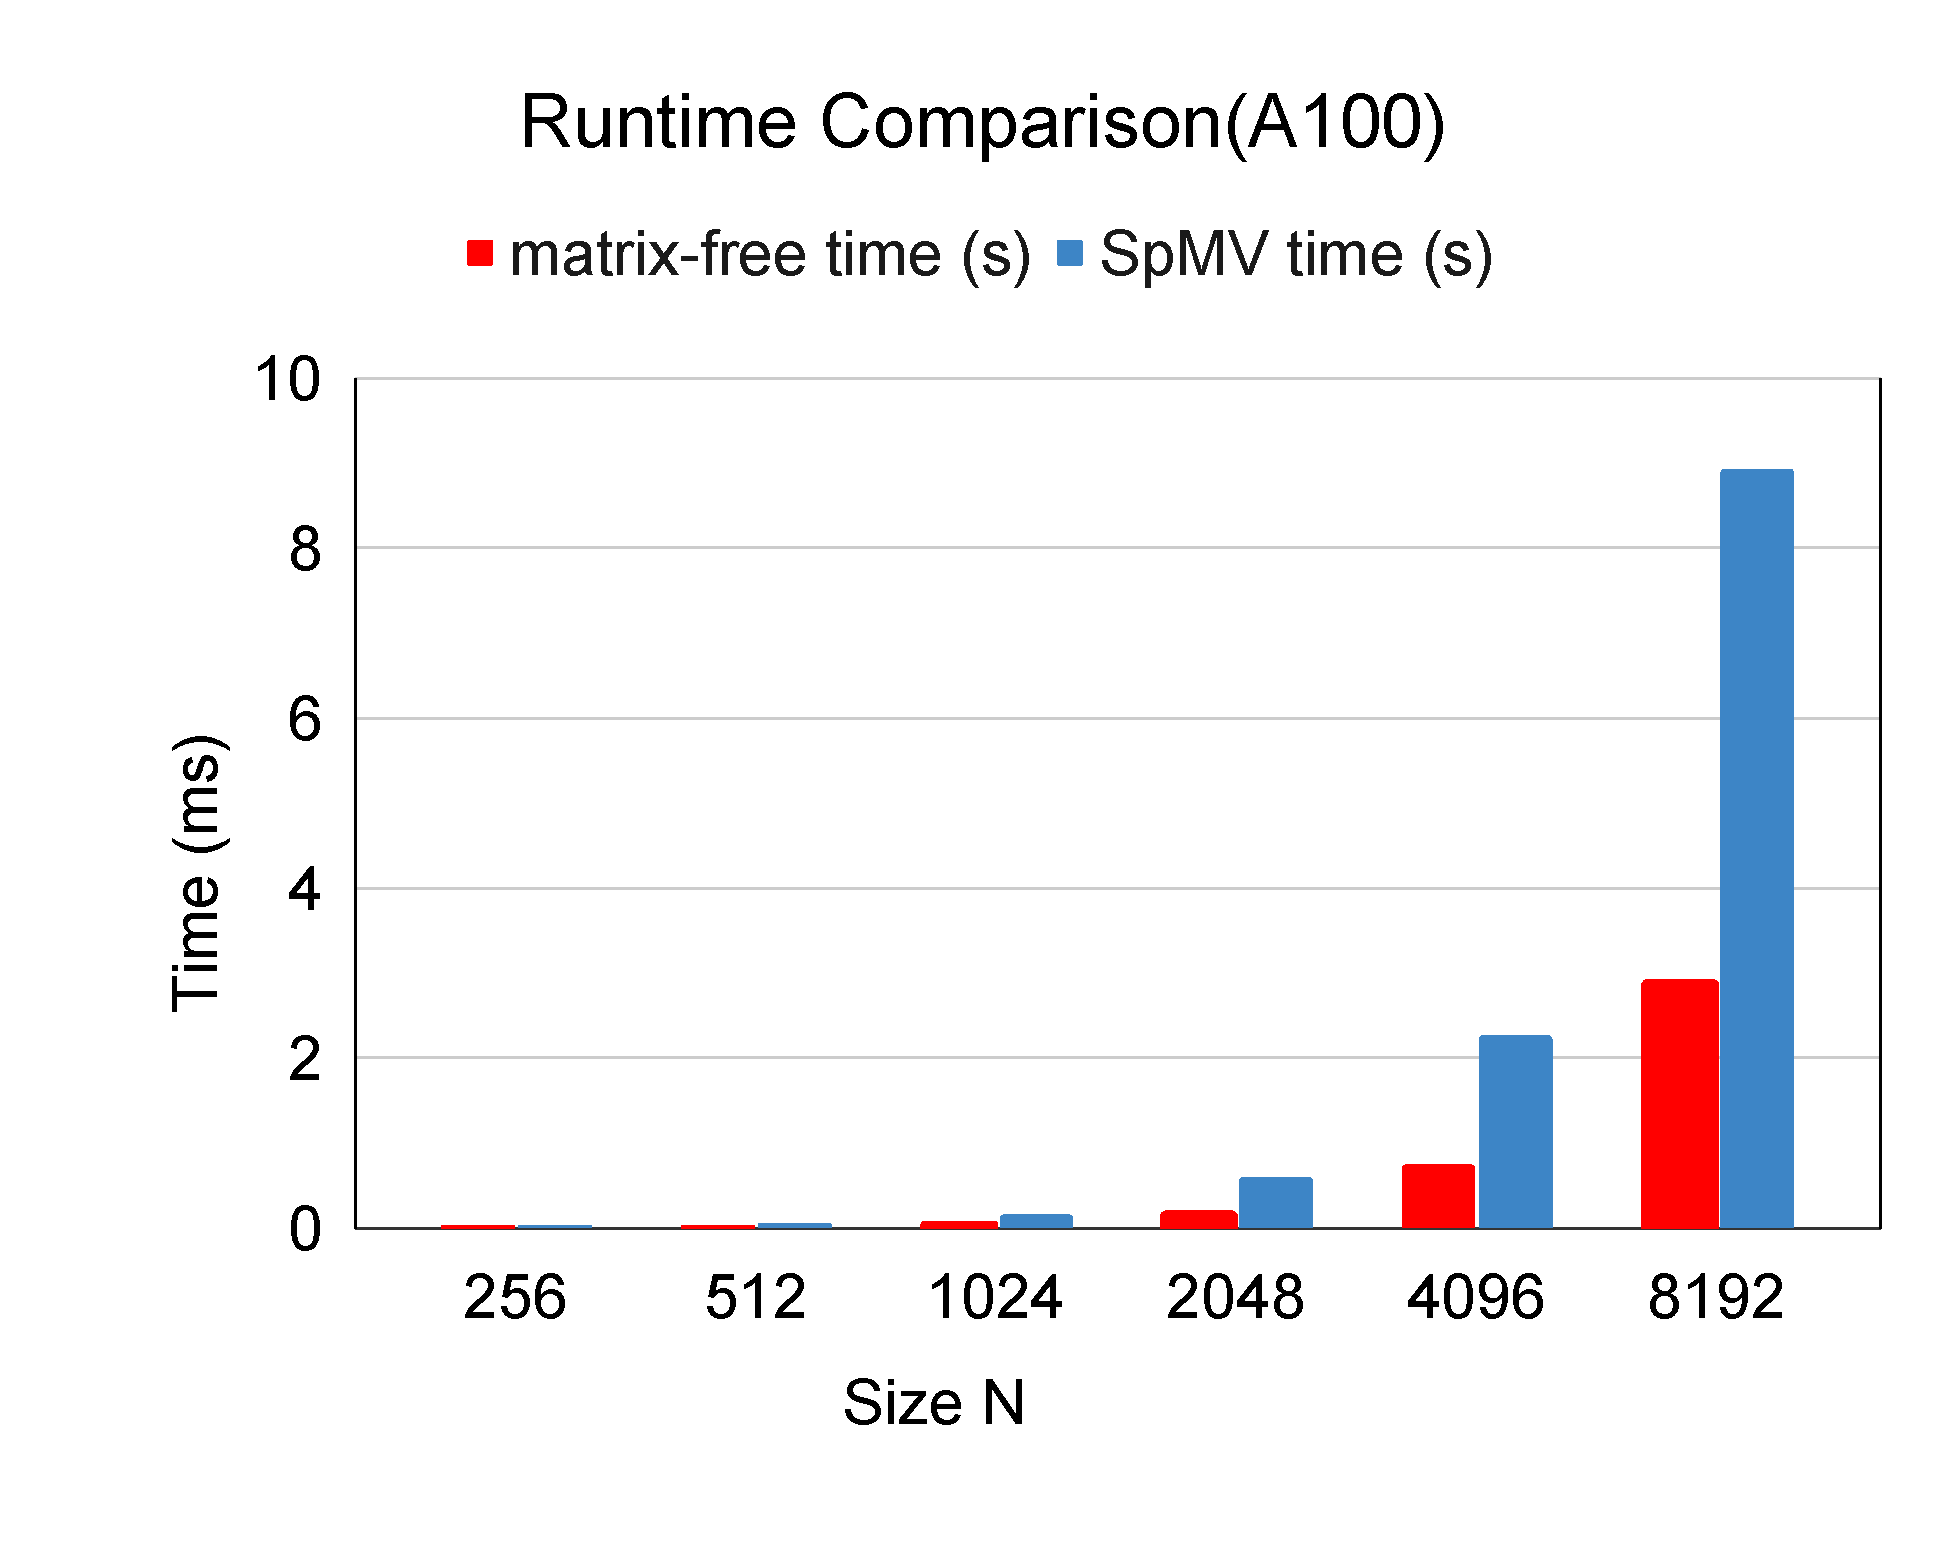
\includegraphics[width=\linewidth]{figures/Runtime_Comparison_A100.pdf}
    \caption{Performance of SpMV vs matrix-free $\texttt{mfA!}$() on A100 GPU. Total time for matrix-free (red) and matrix-explicit CSR (blue) formats are shown in charts plotted against $N$, where the matrix is size $(N+1)^2 \times (N+1)^2$.}
    \label{fig:A100}
\end{figure}

\begin{figure}
    \centering
    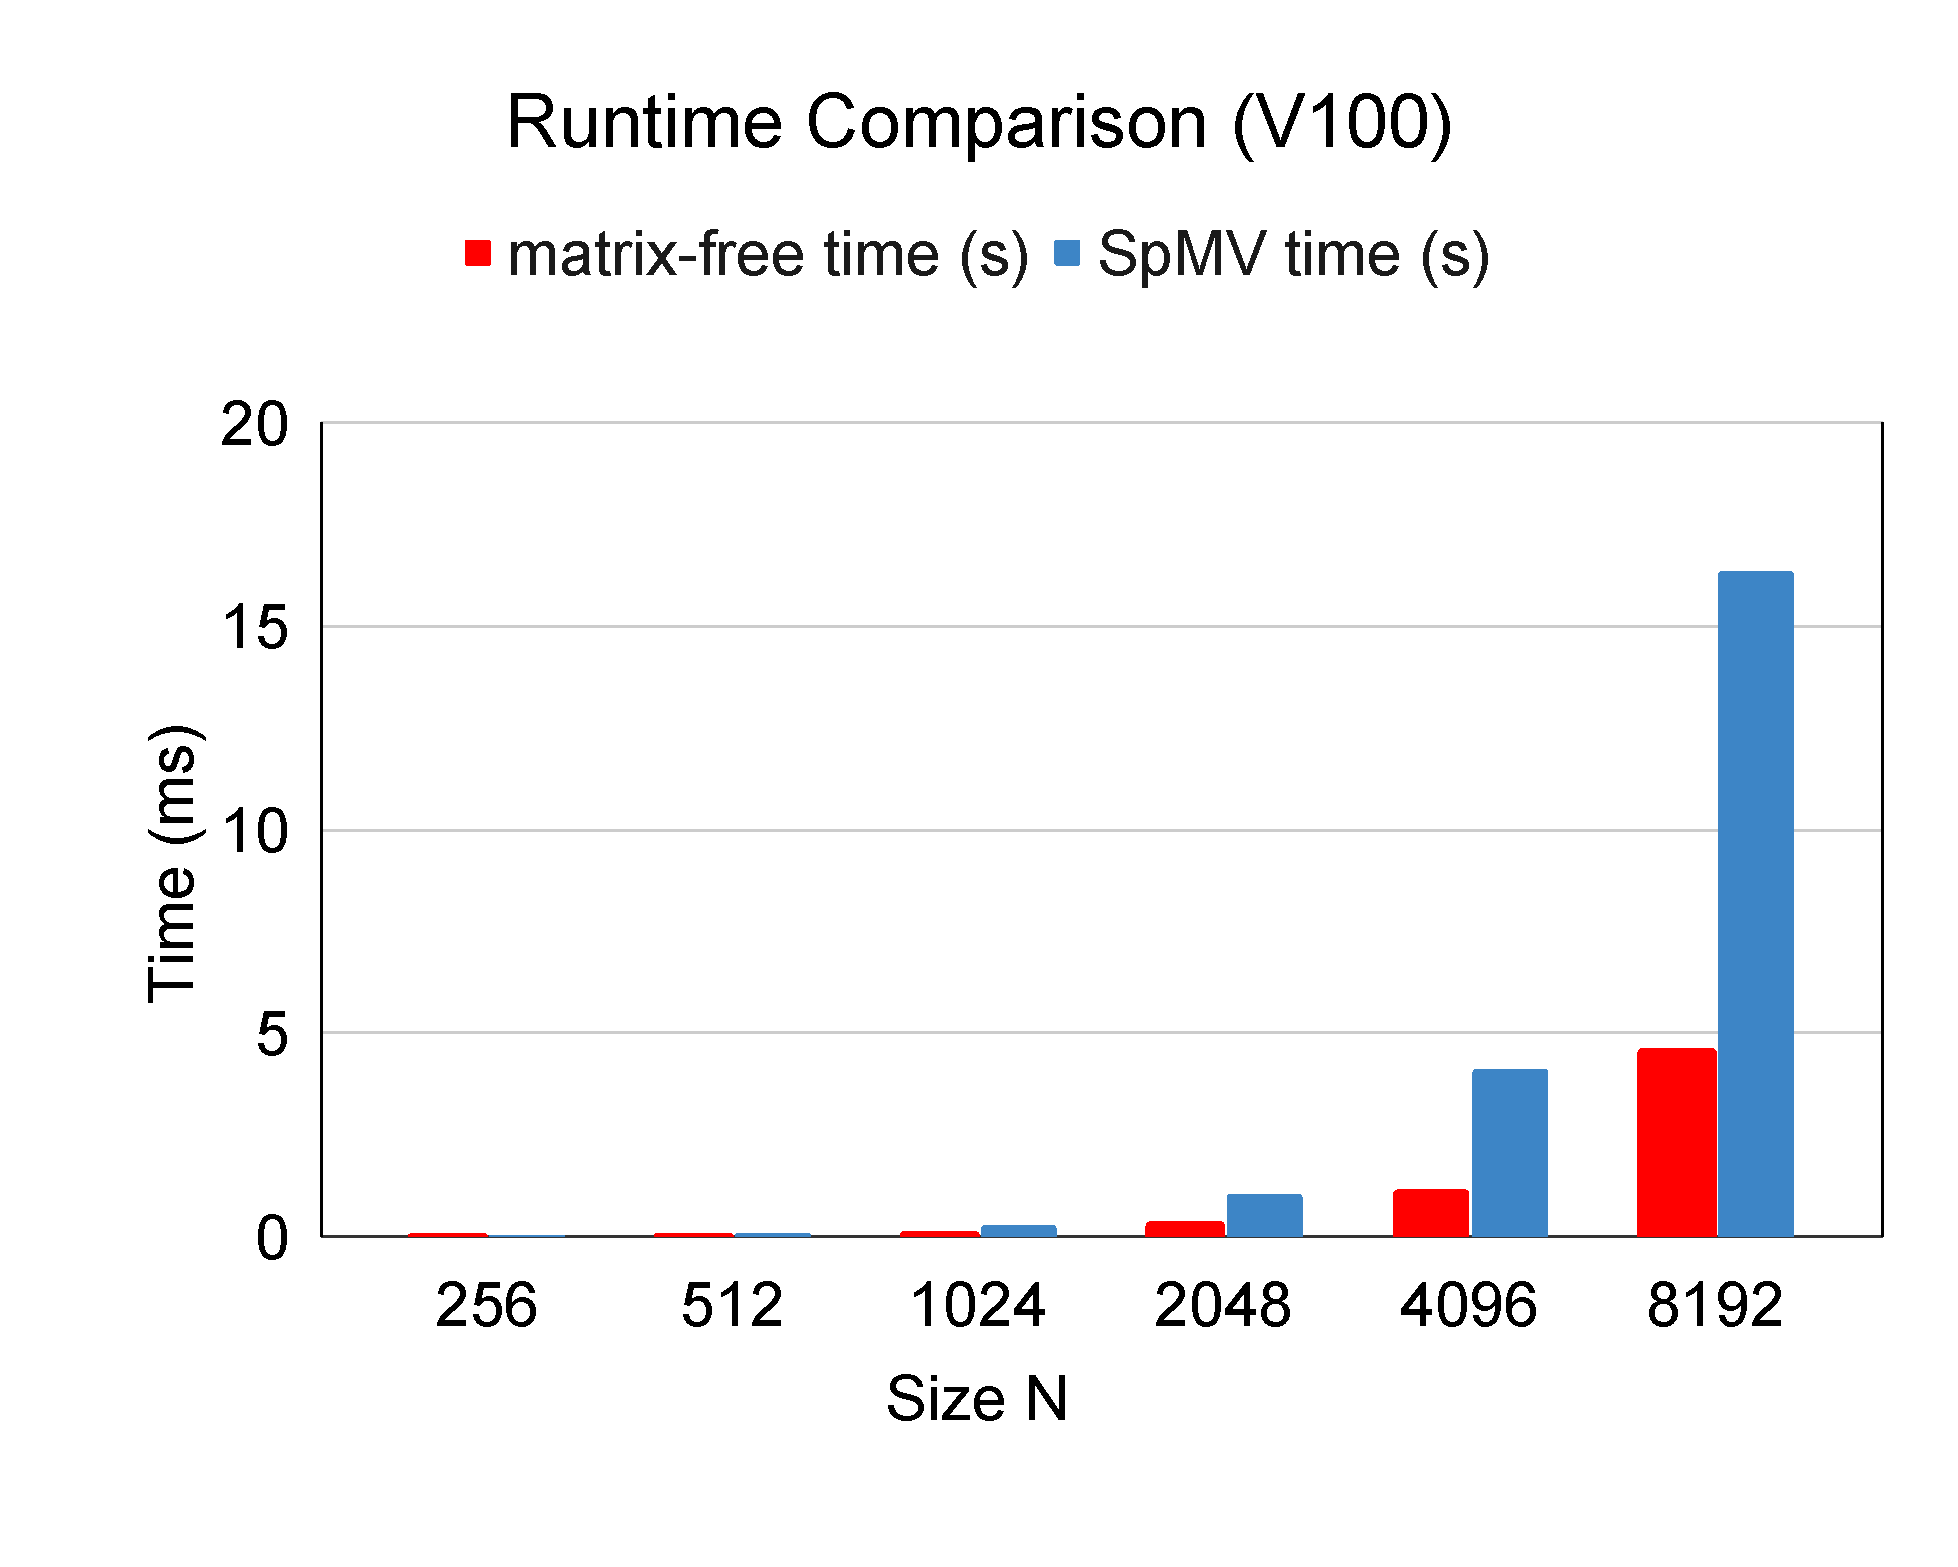
\includegraphics[width=\linewidth]{figures/Runtime_Comparison_V100.pdf}
    \caption{Performance of SpMV vs matrix-free $\texttt{mfA!}$() on V100 GPU. Total time for matrix-free (red) and matrix-explicit CSR (blue) formats are shown in charts plotted against $N$, where the matrix is size $(N+1)^2 \times (N+1)^2$.}
    \label{fig:V100}
\end{figure}

\begin{figure}
    \centering
    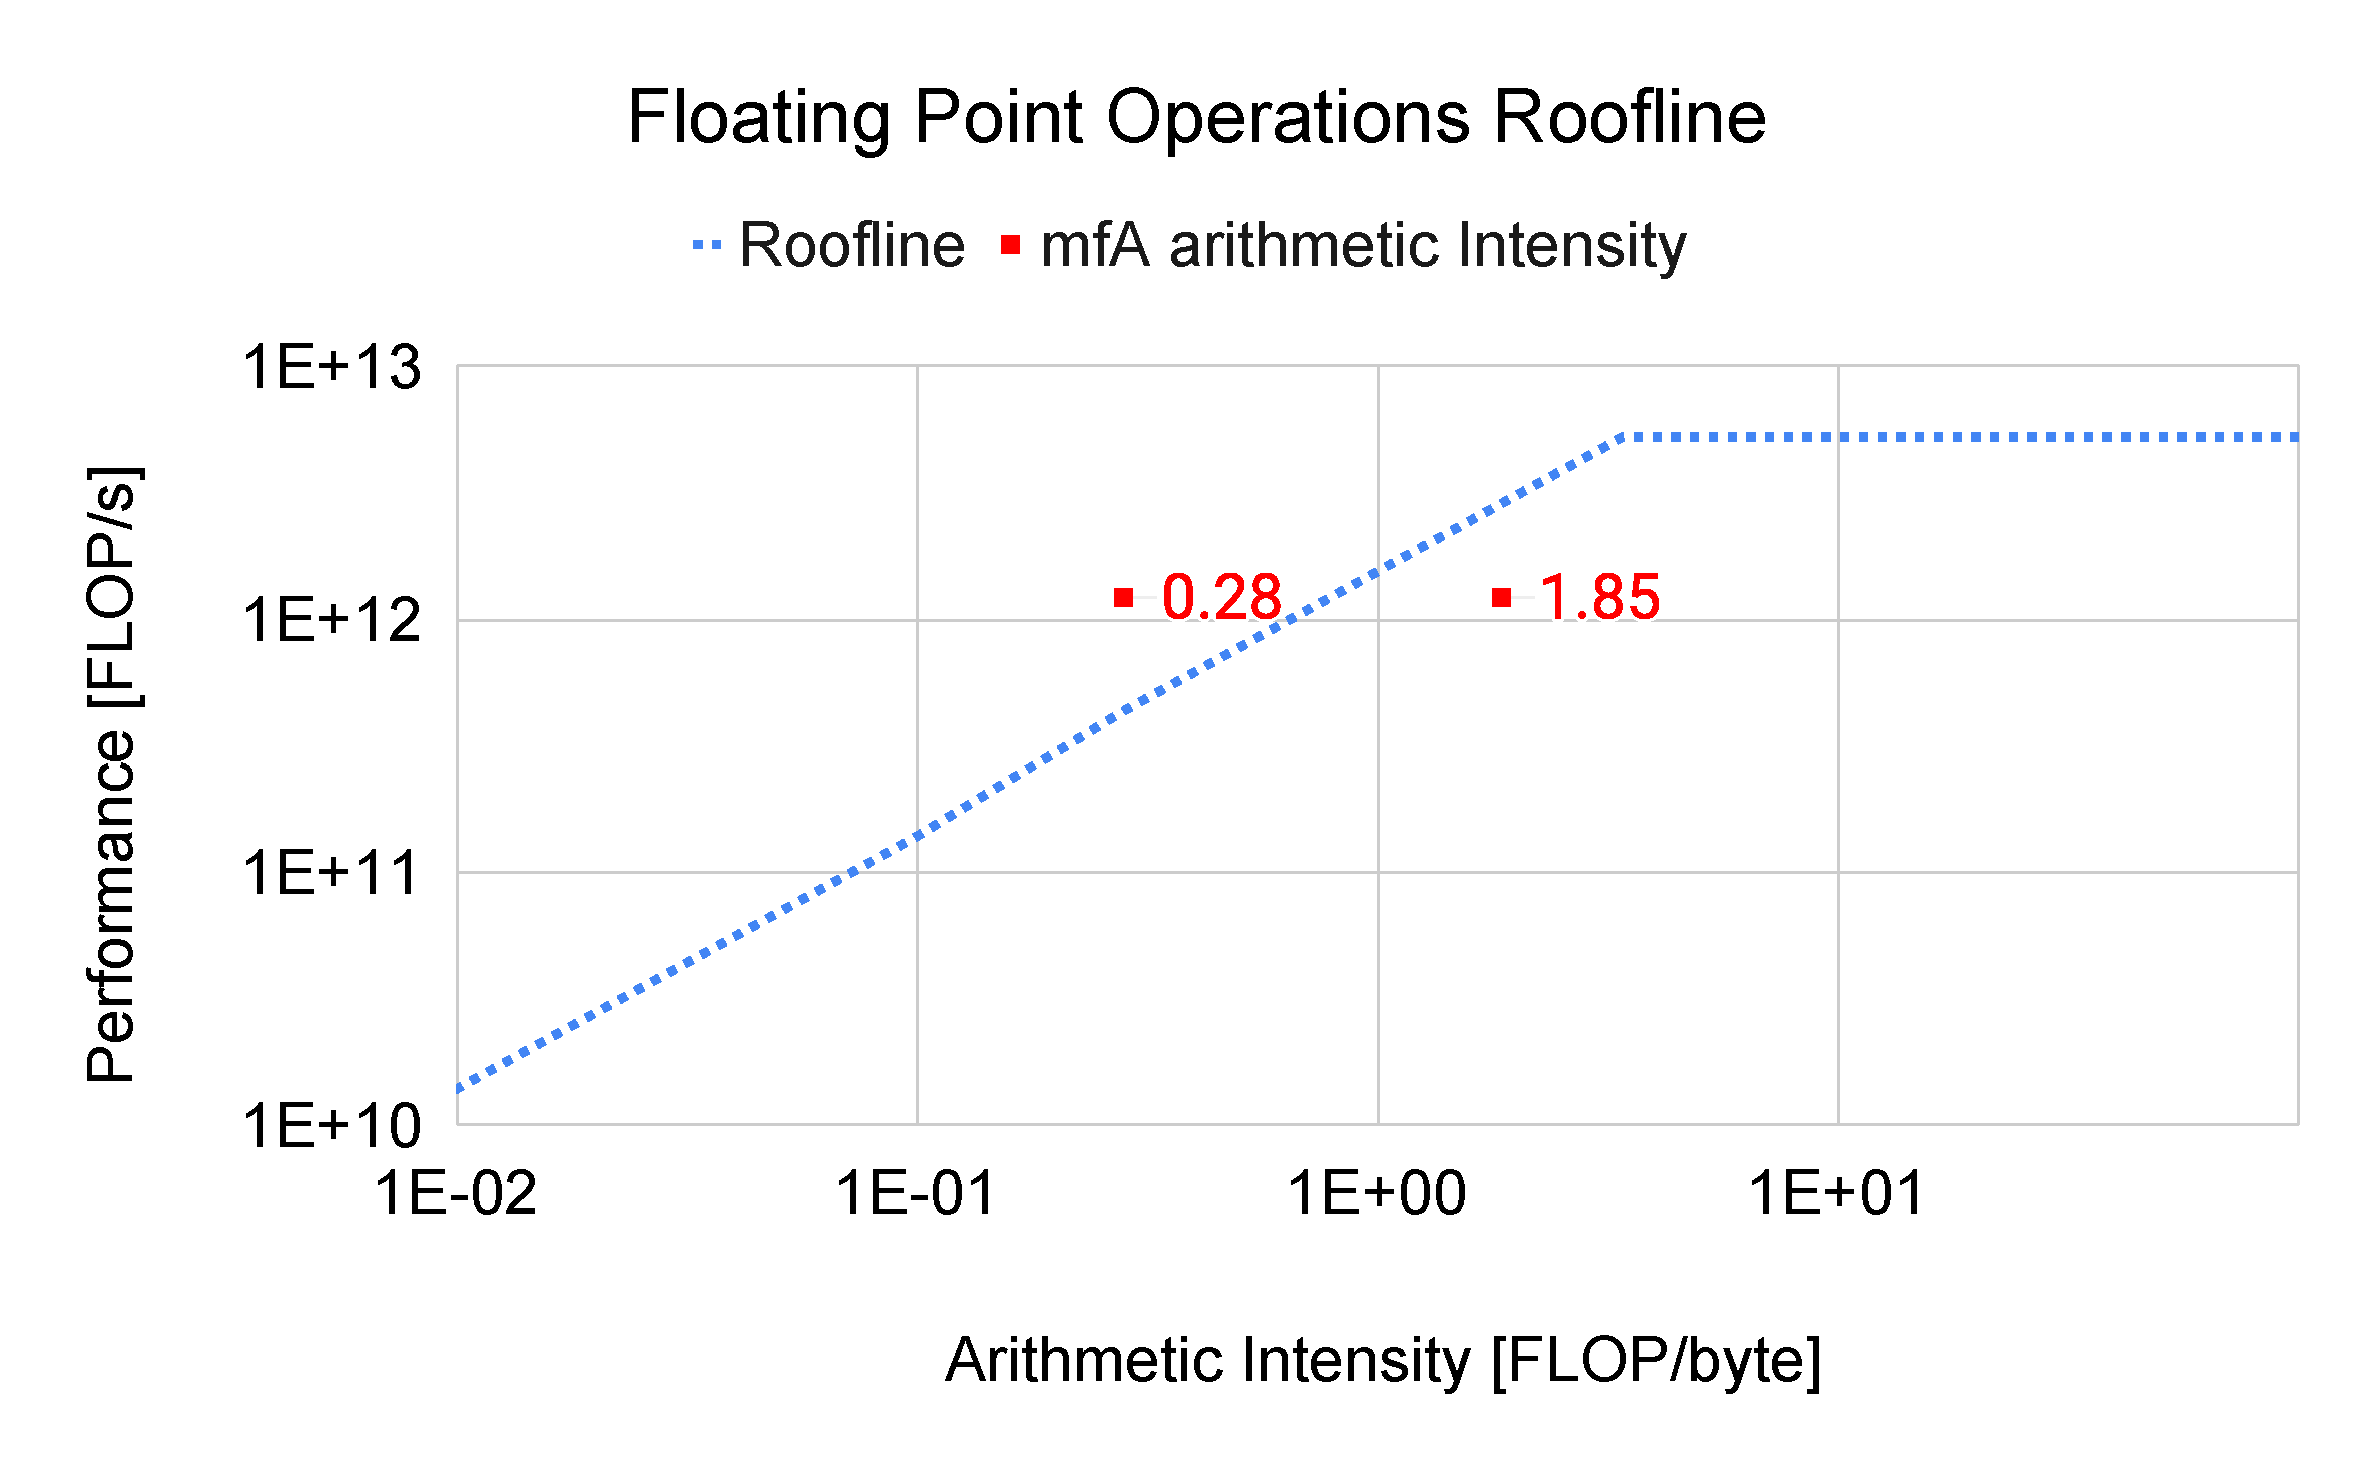
\includegraphics[width=\linewidth]{figures/Floating_Point_Operations_Roofline_Theoretical.pdf}
    \caption{
    Roofline model analysis for our matrix-free $\texttt{mfA!}$() on the A100 GPU.
    The red dot on the left represents the performance achieved by our kernel and its arithmetic intensity (0.28).
    The red dot on the right represents the same but assuming data is loaded only once from DRAM (i.e., compulsory misses), which yields a higher arithmetic intensity (1.85).
    The fact that our kernel (red dot) achieves higher performance than what is predicted by the Roofline model suggests that a large portion of our data is coming from the caches.
    %Roofline analysis for double-precision achieved value from Nsight Compute (blue dotted line) for the matrix-free kernel and theoretical arithmetic intensity for mfA kernels (red points). The left point counts all memory accesses to L1, L2 caches, and DRAM. The right point counts only access to DRAM and assumes the mfA!() kernel reads each data from DRAM only once.
    }
    \label{fig:roofline}
\end{figure}

\begin{figure}
    \centering
    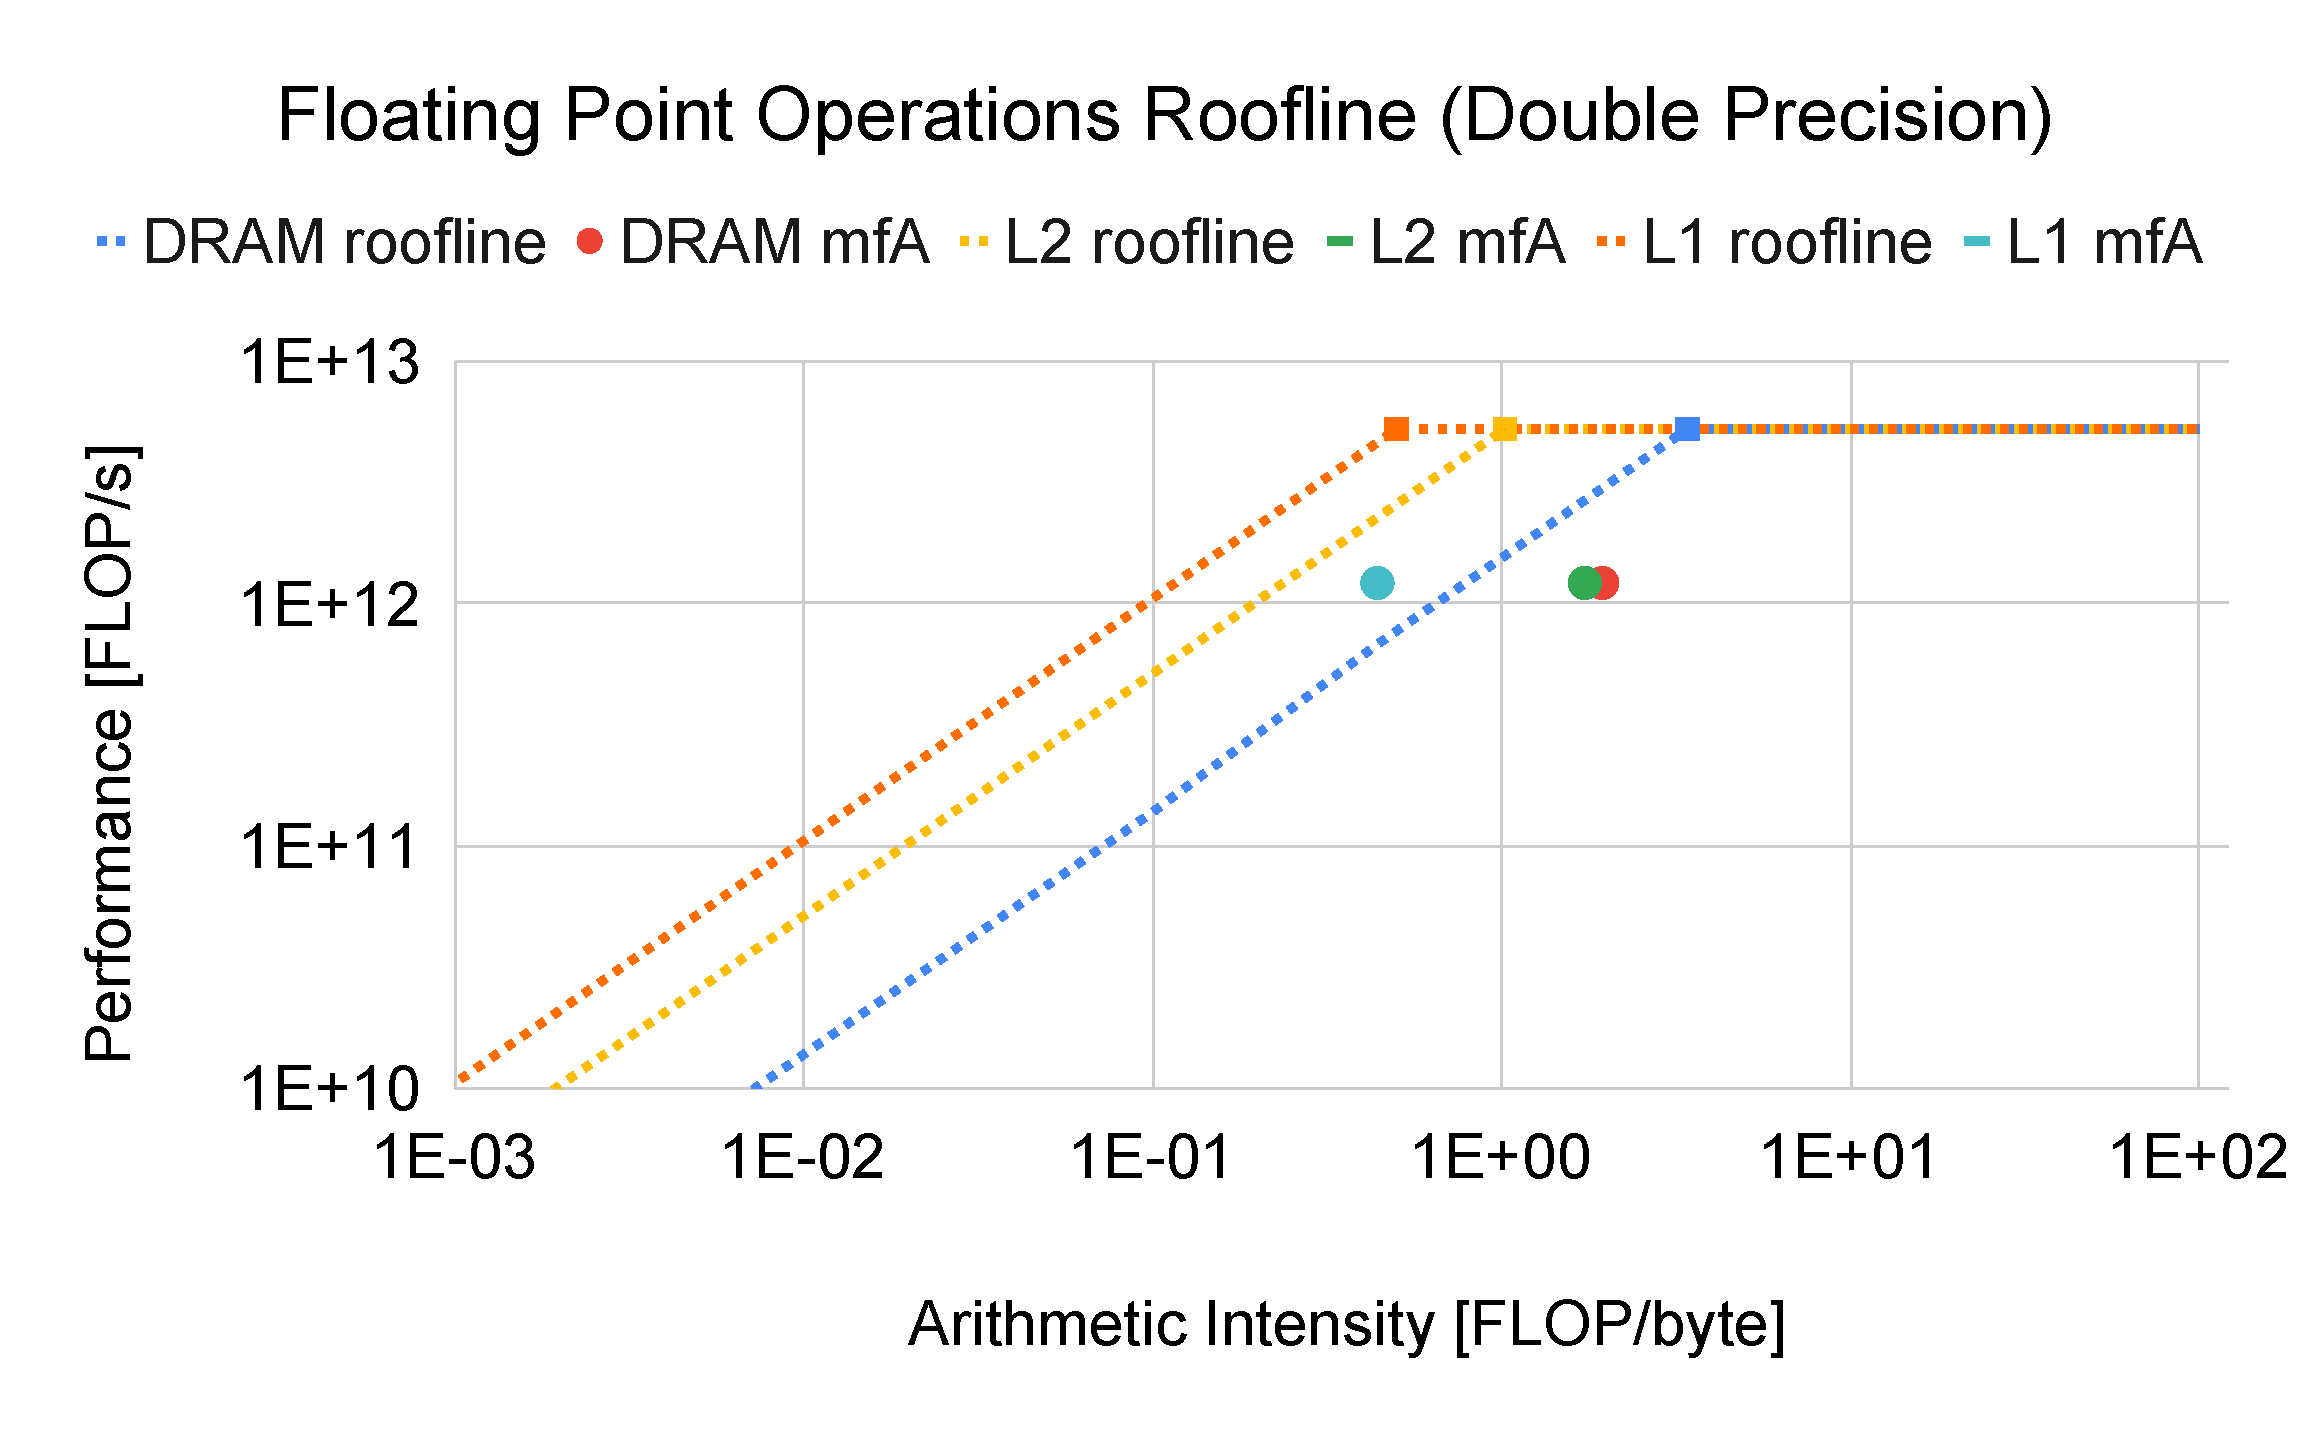
\includegraphics[width=\linewidth]{figures/Floating_Point_Operations_Roofline_Double_Precision.pdf}
    \caption{
    Roofline model generated by Nsight Compute, based on performance counter measurements of how much of the overall data is coming from different levels of the memory hierarchy.
    This confirms our hypothesis that the majority of our data is coming from the L1 cache, and that further improving data reuse in L1 will yield up to $3.8\times$ speedup.
    %Hierarchy roofline analysis for L1, L2, and DRAM (circles from left to right) double-precision achieved values from Nsight Compute for the matrix-free kernel.
    }
    \label{fig:roofline-double-precision}
\end{figure}




\subsection{Memory Usage Comparison}
Next we compare the memory usage of {\ttfamily mfA!}() against the SpMV kernel via the built-in memory status function in CUDA.jl. 
CUDA.jl currently has good support for only three different sparse matrices: CSR, CSC, and COO.
In Julia, the default sparse matrix format is CSC, but in CUDA.jl, the default sparse matrix format is CSR, and thus, there is a necessary conversion between these two formats when converting the CPU arrays to GPU arrays in Julia. 
%However, the actual memory requirement is very similar as these two formats are the transpose of each other. 
However, for our problem, where the matrix is SPD, both CSR and CSC formats use exactly the same amount of memory; the only difference is in the use of row pointer \texttt{rowptr} values (for CSR) instead of column pointer values \texttt{colptr} (for CSC), and the order of nonzero values \texttt{nzval}. 
%stored.
To avoid redundancy, we merge key results in memory consumption for CSC and CSR formats into three different numbers for each $N$.
The collected data is given in \autoref{tab:memalloc_comparison}. 
\label{sec:mem_comp}


\begin{table}[t]
\small\sf\centering
\begin{center}
\begin{tabular}{l l l l l }
\toprule
$N$  & m & nzval & memory size \\
\midrule
$2^{10}$& 1050625  & 9447429 & 0.1596 GB \\
$2^{11}$ & 4198401 & 37769221& 0.6379 GB &  \\
$2^{12}$ & 16785409   & 151035909   & 2.5509 GB &  \\
$2^{13}$ & 67125249   & 604061701   & 10.2020 GB & \\
\bottomrule
\end{tabular}
\end{center}
\caption{Number of nonzero values (nzval) for CSC or CSR sparse matrices with different $N$, where matrix size is $(N+1)^2 \times (N+1)^2$. The matrices are SPD. Here, m represents the number of rows, and nzval represents the number of nonzero values. The total memory size (last column) is calculated using previous columns.
}
\label{tab:memalloc_comparison}
\end{table}


\begin{table}[t!]
\small\sf\centering
\begin{center}
\begin{tabular}{l l l l l }
\toprule
$N$  & crr/css/crs & $\Psi_1$/$\Psi_2$ & total memory size \\
\midrule
$2^{10}$& 0.008405 GB  & 8 KB & 0.02523 GB \\
$2^{11}$ & 0.03359 GB & 16 KB &  0.1008 GB \\
$2^{12}$ & 0.1343 GB  & 32 KB  & 0.4029 GB &  \\
$2^{13}$ & 0.5370 GB   & 65 KB   & 1.6111 GB & \\
\bottomrule
\end{tabular}
\end{center}
\caption{Memory allocation for matrix-free methods where matrix size is $(N+1)^2 \times (N+1)^2$. Here $\mathrm{crr}$, $\mathrm{css}$, and $\mathrm{csr}$ correspond to coefficient matrices of size $(N+1)^2$. $\Psi_1$ and $\Psi_2$ are used in Dirichlet boundary conditions and are vectors of length $N+1$. Total memory allocated (last column) is calculated using previous columns.
}
\label{tab:memalloc_mf}
\end{table}

For the matrix-free method, memory consumption is reported in \autoref{tab:memalloc_mf}. 
In order to perform the matrix-vector product, we need to allocate memory to store the coefficients $c_{rr}$, $c_{ss}$ and $c_{rs}$; each requires the same size of memory as the numerical solution and must be stored on each grid level when using geometric multigrid as a preconditioner. 
In addition, we must compute and store the minimum coefficient values ${\boldsymbol{C}}_{rr}^{k, min}$ on faces 1 and 2, as specified in the previous section, which we denote $\Psi_1 = $ and $\Psi_2$, respectively. 


These are associated with Dirichlet boundary conditions and are significantly smaller in size, and thus reported in KB. Adding up these contributions, we can compute the total memory size, which we provide in the last columns of Tables \autoref{tab:memalloc_comparison} and \autoref{tab:memalloc_mf}: We can see that there is a significant reduction in additional required memory for the matrix-free method than the memory to store sparse matrices in CSC or CSR format. When calculating the total memory used for an SpMV operation (including writing results into output vectors), we need to add additional memory allocated for the input data and output data, which require the same memory as the coefficients (the first column of \autoref{tab:memalloc_mf}). A simple calculation can show that the total memory required when using an SpMV kernel is a constant $4.2\times$ of that required for the matrix-free method. 
\section{Performance: Matrix-free MGCG on GPUs}\label{sec: conjugate}


\begin{table*}
    \caption{Time to perform a direct solve after LU factorization on CPUs vs PCG on GPUs. We report time in seconds and iterations to converge. For AmgX, we report setup + solve time. For our MGCG, setup time is negligible. ``$\mathrm{ns}$'' is short for the number of smoothing steps. GPU results are tested on A100.}
    \small
    \centering
    \begin{tabular}{rrrrrr}
    \toprule
    $N$     & Direct Solve  & AmgX (ns = 1) & AmgX (ns = 5)  & SpMV-MGCG (ns = 5)   & MF-MGCG (ns = 5)\\
    \midrule
    $2^{10}$  &   0.912 s & (0.0319 s + 0.0243 s) / 25  & (0.0321 s + 0.0435 s) / 17  & 7.019E-2 s / 8   & 2.851E-2 s / 8       \\
    $2^{11}$ & 6.007 s &  (0.086 s + 0.161 s) / 55   &  (0.086 s + 0.311 s) / 38   & 0.158 s / 7  & 0.0605 s / 7     \\
    $2^{12}$ & 22.382 s  & (0.310 s + 0.235 s) / 24  &  (0.323 s + 0.488 s) / 15      & 0.564 s / 7  & 0.207 s / 7         \\
    $2^{13}$ & 134.697 s  & (1.334 s + 1.643 s) / 24   & (1.217 s + 1.865 s) / 16   & 5.028 s / 7   & 0.865 s / 7      \\
    \bottomrule
    \end{tabular}
    \label{tab:mgcg}
    
\end{table*}

With the matrix-free action of $\boldsymbol{A}$ established, we can solve system \eqref{eqn: final} with a matrix-free version of our custom MGCG method (MF-MGCG). 
Other than low-level GPU kernels, Julia also supports high-level vectorization for GPU computing, which we utilize extensively in our MGCG code for convenience.
In this section, we compare its performance against MGCG using the cuSPARSE (matrix-explicit) SpMV (SpMV-MGCG) and also against the state-of-the-art off-the-shelf methods offered by NVIDIA, namely, AmgX - the GPU accelerated algebraic multigrid. The solvers and preconditioners used by AmgX are stored as JSON files. 
We explored different sample JSON configuration files for AmgX in the source code and found that CG preconditioned by classical AMG performed best for our problem. 
To maintain a multigrid setup comparable to our MGCG, we modified the \texttt{PCG\_CLASSICAL\_V\_JACOBI.json} to use 1 and 5 smoothing steps with block Jacobi as the smoother.
% and remove aggressive coarsening. 
All algorithms stop when the relative residual is reduced to less than $10^{-6}$ times the initial residual.
We report our results in Table \ref{tab:mgcg}. Also included in the table are results using a direct solve (using LU factorization in LAPACK in Julia) only because it is so often used in the earthquake cycle community for volume based codes \cite{erickson2020community} and our developed methods offer promising alternatives. As illustrated, the GPU-accelerated iteratives schemes achieve much better performance for the problem sizes tested.

Table \ref{tab:mgcg} illustrates that our MGCG method uses fewer iterations to converge compared to AmgX, while iterations for both remain generally constant with increasing problem size. When we increase smoothing steps from 1 to 5, the AmgX sees reduced iterations, but the time to solve also increases by roughly $3\times$.
%This increase in time to solve is more noticeable for smaller problems with $N=2^{10}, 2^{11}, 2^{12}$.
Because we apply rediscretization (rather than Galerkin coarsening) for MGCG, the setup time is negligible.
The setup time in the AmgX is comparable to the solve time however, which adds additional cost to use AmgX as a solver.
Our SpMV-MGCG is roughly 2$\times$ slower than the AmgX using 1 smoothing step, but our MF-MGCG is faster than AmgX, up to $2\times$ speedup for $N = 2^{13}$.
Compared to our SpMV-MGCG, our MF-MGCG achieves more than $2\times$ speedup, and the speedup is more obvious at $N=2^{13}$, indicating that the MF-MGCG is suitable for large problems.


In this chapter, we present a matrix-free implementation of the multigrid preconditioned conjugate gradient in order to solve 2D, variable coefficient elliptic problems discretized with an SBP-SAT method.
Our customed multigrid preconditioner achieves similar preconditioning performance against the multigrid using Galerkin's condition from previous work, and it is more suitable for GPU code.
The MGCG algorithm requires a nearly constant number of iterations to converge for various problem sizes. 
We used Nsight Compute to analyze the performance of our matrix-free kernel. This offers us more insights into the achieved computation and memory performance, which points to directions for future kernel-level optimizations on newer GPU architectures.

This work is a fundamental first step towards high-performance implementations to solve linear systems using SBP-SAT methods. Future work will target SBP-SAT methods with higher-order accuracy in 3D, as well as explorations of additional GPU kernel optimization and multi-GPU implementation. We also plan to improve the performance of the preconditioner by systematic experiments with different preconditioner configurations using PETSc and applying second-order smoothers that have exhibited improved performance in the multigrid method as well as the mixed-precision techniques ~\cite{golub1961chebyshev,gutknecht2002chebyshev,abdelfattah2021survey}.

%%--- Chapter 5 ---------------------------------------------------------------%
\chapter{SEAS benchamrk problems}
% \section{Chapter Three Section One}
% \subsection{Chapter three section one sub-section one}
% \subsubsection{Chapter three section one sub-section one sub-sub-section one}
\section{SEAS problems}
\subsection{Modeling Environment}
The applications are motivated by the study of quasi-static deformation of the solid Earth over the time scales of earthquake cycles.
In both the interseismic and coseismic phases, the off-fault material response is modeled as elastic-plastic.
\begin{equation}\label{eqn:governing}
    \rho \ddot{u} = \nabla \cdot \sigma + F, \sigma = \boldsymbol{C} : (\epsilon - \epsilon^p) 
\end{equation}

Here, $\rho$ is the material density, $u$ is the vector of particle displacements, $F$ is the body fordce, $\boldsymbol{C}$ is the stiffness tensor of elastic moduli, and $\epsilon$ and $\epsilon^p$ are the elastic and plastic strains.
\begin{figure}
    \centering
    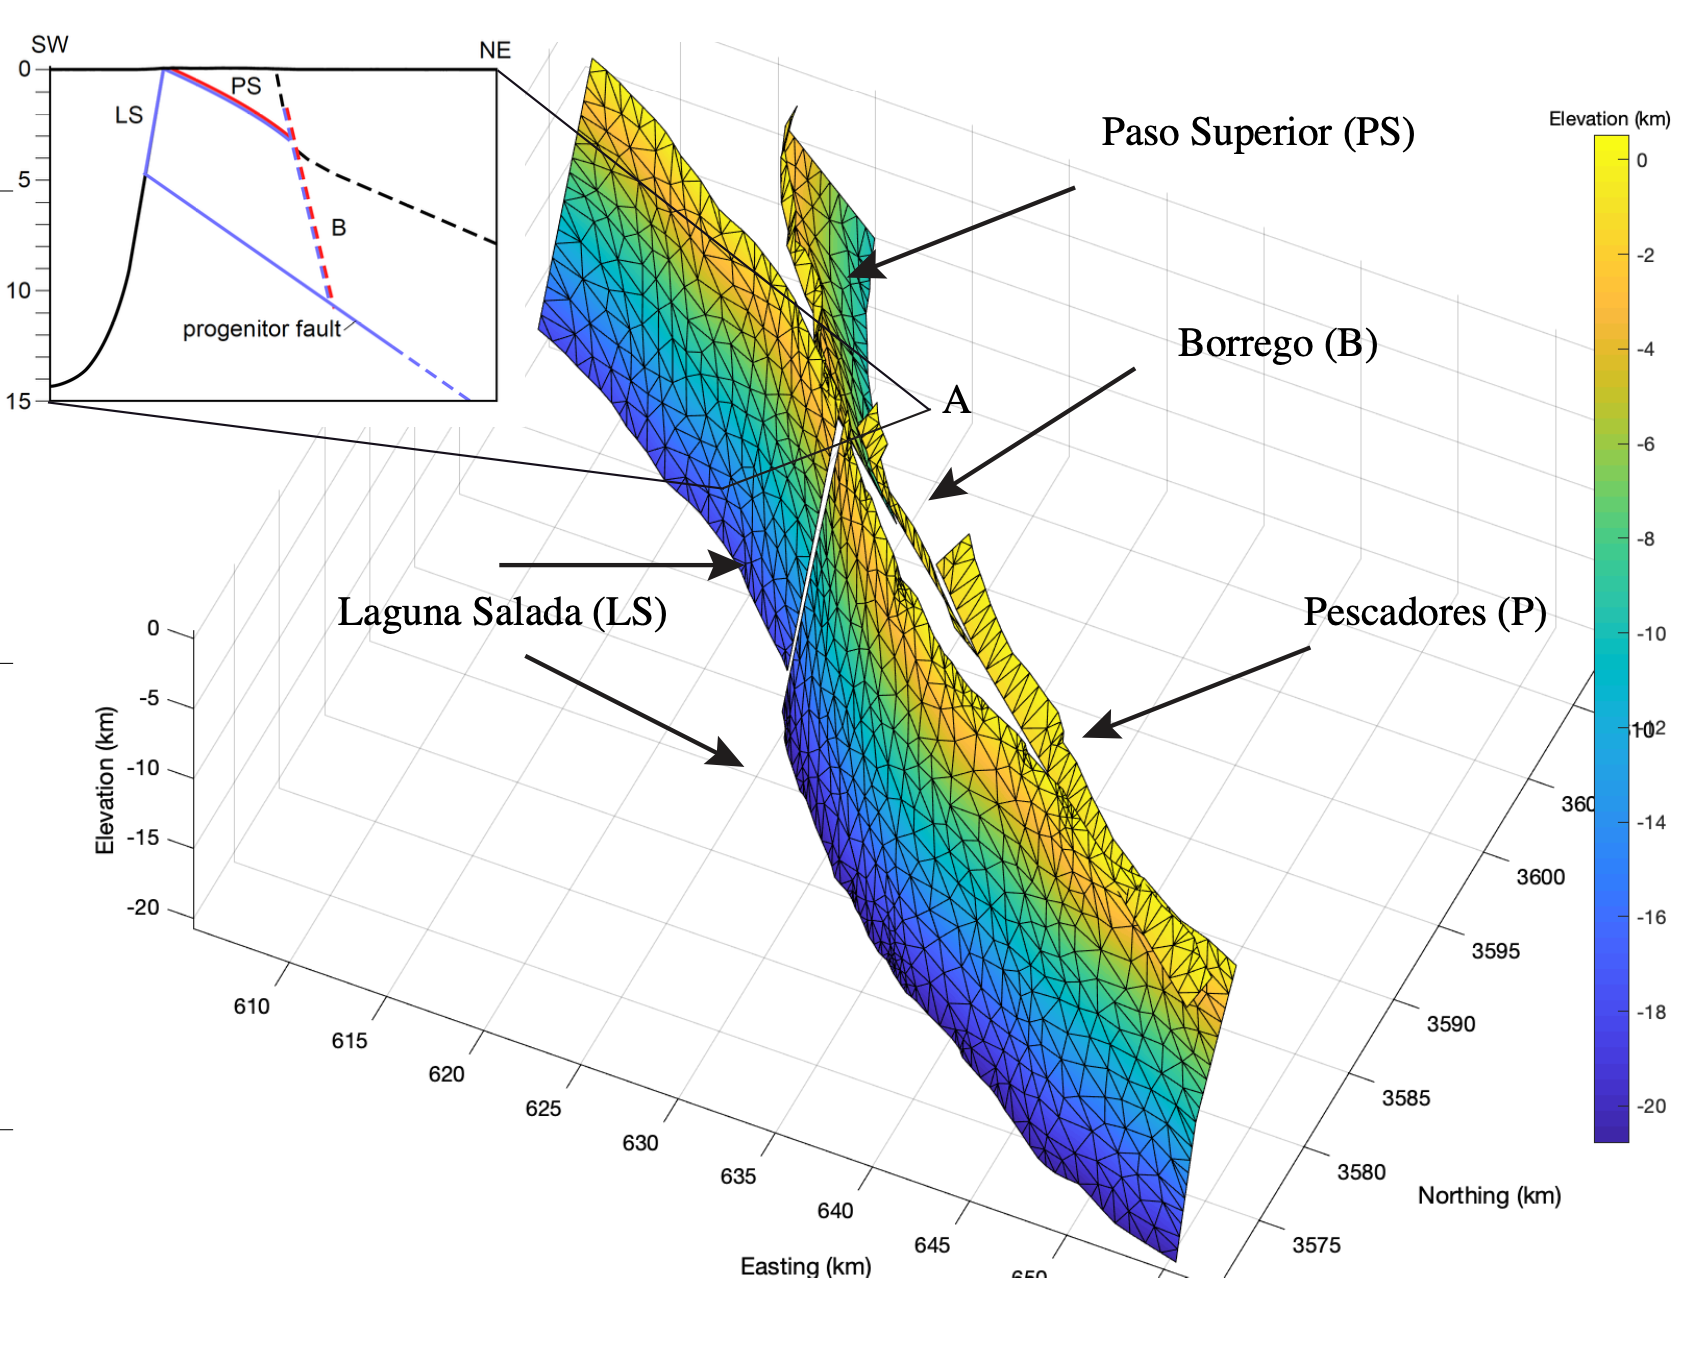
\includegraphics[width=\linewidth]{figures/fault-network.png}
    \caption{A 3D image of the complex fault network from EMC earthquake; image generated using scripts from \citep{https://doi.org/10.1002/2016GL072289}}
    \label{fig:fault-network}
\end{figure}
A fault network (an example shown in \autoref{fig:fault-network}) is composed of faults governed by non-linear, rate-and-state friction which determines the relationship between the slip velocity $V$ to shear traction $\tau$ with the (effective) norm stress $\bar{\sigma}$, the friction coefficient $f$ and a state variable $\Psi$.
\begin{equation}\label{eqn:friction-law}
    \tau = \bar{\sigma} f(V,\Psi), \Psi = G(V, \Psi)
\end{equation}
The form of the state evolution law $G$ can take several forms such as the aging law in which the state evolves in the absence of slip or the slip law with strong rate-weakening.

During the interseismic phase, the inertial terms in the governing \autoref{eqn:governing} are set 0 ($\ddot{u} = 0$).
Tectonic loading is imposed through time-dependent boundary conditions and the slip on faults are incorporated through friction law \autoref{eqn:friction-law}.
The evolution of $\Psi$ constraints the time step, and very large time steps can be used during the interseismic phase.
The main computational challenge comes from solving the large linear systems of equations that come from the discretization of the steady-state version of the \autoref{eqn:governing}.
During the interseismic phase, tectonic loading determines the boundary conditions and the stress on faults as the result of elastic deformation.
Once an event begins to nucleate, we enter the coseismic phase and inertial terms of governing \autoref{eqn:governing} are retained.
It is more efficient to use explicit integration during this period because it simplifies the computation. In both phases, the governing equation can be solved using the SBP-SAT methods mentioned in the previous section.

\subsection{3D Problem Setup}
The 3D problem setup described below is taken from previous SEAS publications \citep{10.1785/0220190248}.
The medium is assumed to be a homogeneous, isotropic, linear elastic half-space defined by
\begin{equation} \label{eqn:domain}
    \textbf{x} = (x_1, x_2, x_3) \in (-\infty, \infty) \times (\infty, \infty) \times (0, \infty)
\end{equation}
with a free surface at $x_3 = 0$ and $x_3$ as positive downward. A vertical, strike-slip fault is embedded at $x_1 = 0$, We use the notation ``+'' and ``-'' to refer to the different sides of the fault. 

We assume 3D motion, letting $u_i = u_i(\textbf{x}, t), i = 1, 2, 3$ denote the displacement in the $i$-direction.
Hooke’s law for linear elasticity is given by
\begin{equation}
    \sigma_{ij} = K\epsilon_{kk}\delta_{ij} + 2\mu (\epsilon_{ij} - \frac{1}{3} \epsilon_{kk}\delta_{ij})
\end{equation}
for bulk modulus $K$ and shear modulus $\mu$. The strain-displacement relations are given by 
\begin{equation}
    \epsilon_{ij} = \frac{1}{2} \left[\frac{\partial u_i}{\partial x_j} + \frac{\partial u_j}{\partial x_i}\right]
\end{equation}
The description of these benchmark problems can be found in \citep{erickson2018seas,jiang2020seas}.
To simulate the SEAS problems using the quasi-static method, it usually follows these steps.

\begin{algorithm}
    \caption{Quasi-static Formulation Algorithm}
    \begin{algorithmic}[1]
        \State \textbf{Step 1:} Initialize boundary conditions and state variables
        
        \While{simulation time not reached}
            \State \textbf{Step 2:} Solve steady-state problems to obtain displacements
            % \State \hspace{1em} In 2D, Solve Poisson's equation
            % \State \hspace{1em} In 3D Solve linear elasticity
            \State \hspace{1em} Linear solve of equations of static elasticity
            
            \State \textbf{Step 3:} Calculate stress from displacements
            
            \State \textbf{Step 4:} Calculate slip velocity using rate-and-state friction
            
            \State \textbf{Step 5:} Determine time step size ($dt$) using ODE solver
            
            \State \textbf{Step 6:} Integrate state variables using aging law and $dt$
            
            \State \textbf{Step 7:} Update boundary conditions using slip velocity and $dt$
        \EndWhile
    \end{algorithmic}
\end{algorithm}

The DifferentialEquations.jl package provides powerful adapted ODE solvers based on Runge-Kutta methods and useful ODE interfaces that allow us to modify data and write to outputs.
The key challenge here is step 2 which requires solving a large linear system that is formed with the SBP-SAT methods.
It's difficult to apply direct methods due to their high memory requirements and computational inefficiency. 
In the next two chapters, we will go into detail to first formulate the linear systems using the SBP-SAT methods and then apply HPC algorithms to solve such problems.


\subsection{Solving for rate-and-state friction}
Rate-and-state friction plays a central role in all SEAS problems. 
The friction coefficient function $f$ in SEAS problems is given as a regularized formulation
\begin{equation}
    f(V, \theta) = a \sinh^{-1} [\frac{V}{V_0} \exp{\frac{f_0 + b \ln(V_0 \theta / L)}{a}}]
    \label{eqn:friction-coefficient}
\end{equation}

$f_0$ represents the reference friction coefficient. $V_0$ represents slip rate, and $a$ and $b$ are rate-and-state parameters. For benchmark problem 1 and 5, $b$ is constant as $b_0$, but $a$ varies throughout computational domain \text{$\Omega$}{$_f$} in order to define velocity-weakening and velocity-strengthening regions. We will define them in respective sections differently.

The state variable $\theta$ evolves according to the aging law
\begin{equation}
    \frac{d\theta}{dt} = 1 - \frac{V\theta}{L}
    \label{eqn:aging-law}
\end{equation}

The fault strength is given as 
\begin{equation}
    \textbf{F} = \bar{\sigma}_n f(V,\theta) \frac{\textbf{V}}{V}
    \label{eqn:fault-strength}
\end{equation}
where \textbf{F} and \textbf{V} are vectors and $V$ is the norm of the \textbf{V}.
The rate-and-state friction where shear stress on fault is equal to fault strength \textbf{F}.
In Quadsi-static simulations, fault displacements are solved given governing equations and boundary conditions. 
Shear stress is calculated using displacements on fault.
In \autoref{eqn:fault-strength} and \autoref{eqn:friction-coefficient}, we can solve for $V$ and then calculate components of $V$ based on components of \textbf{F}. 
This significantly simplifies the calculation and improves numerical accuracy due to the magnitude differences between different components of \textbf{F} and \textbf{V}.

Once all parameters in \autoref{eqn:friction-coefficient} and \autoref{eqn:fault-strength} are known along shear stress calculated from displacements, it is common to apply Newton's method given in Algorithm \autoref{alg:newton} to solve the non-linear equation to obtain $V$.
\begin{algorithm}
\caption{Newton's Method}
\begin{algorithmic}[1]
\State Initialize $x_0$
\State Set tolerance $\epsilon$
\State Set maximum number of iterations $N_{\max}$
\For{$k = 0, 1, 2, \ldots, N_{\max}$}
    \State Compute $f(x_k)$ gradient $\nabla f(x_k)$
    % \State Compute Hessian $\nabla^2 f(x_k)$
    % \If{$\nabla^2 f(x_k)$ is not positive definite}
    %     \State Modify Hessian to be positive definite (e.g., $\nabla^2 f(x_k) + \lambda I$ where $\lambda > 0$)
    % \EndIf
    \State Determine search direction $d_k = -(\nabla f(x_k))^{-1}f(x_k)$
    \State Perform line search to find step size $\alpha_k$ such that $f(x_k + \alpha_k d_k) < f(x_k)$
    \State Update $x_{k+1} = x_k + \alpha_k d_k$
    \If{$\|\nabla f(x_{k+1})\| < \epsilon$}
        \State Convergence achieved
        \State \textbf{break}
    \EndIf
\EndFor
\Return $x_{k+1}$
\end{algorithmic}
\label{alg:newton}
\end{algorithm}

In our problem with high nonlinearity from the $\sinh^{-1}$ function, to improve numerical stability, we also need to apply the ``safe-guarded'' method.
One commonly used method is called bisection, it uses a similar approach to binary search. 
Based on the functional values of a close range $[x_L, x_r]$, it updates the search range of the root $x$.
Newton's method modified with Bisection is given in Algorithm \autoref{agl:newton-bisec}.

\begin{algorithm}
\caption{Newton's Method with Bisection}
\begin{algorithmic}[1]
\State Initialize $x_0$, bounds [$x_L$, $x_R$], and $x = (x_L + x_R) / 2$
\State Set tolerance $\epsilon_a$, $\epsilon_r$ and step size $\alpha_k = x_R - x_L$
\State Set maximum number of iterations $N_{\max}$
\For{$k = 0, 1, 2, \ldots, N_{\max}$}
    \State Compute $f(x_k)$ and gradient $\nabla f(x_k)$
    % \State Compute Hessian $\nabla^2 f(x_k)$
    \State Compute $f_L$, $f_R$ as $f(x_L), f(x_R)$  
    % \If{$\nabla^2 f(x_k)$ is not positive definite}
    %     \State Modify Hessian to be positive definite (e.g., $\nabla^2 f(x_k) + \lambda I$ where $\lambda > 0$)
    % \EndIf
    \State Determine search direction $d_k = -(\nabla f(x_k))^{-1} f(x_k)$
    \State Perform line search to find step size $\alpha_k$ such that $f(x_k + \alpha_k d_k) < f(x_k)$
    \State Update $x_{k+1} = x_k + \alpha_k d_k$
    \If{$x_k < x_L$ or $x_k > x_R$}
        \State $x_k = (x_L + x_R) / 2$
        \State $\alpha_k = (x_R - x_L) / 2$
    \EndIf
    \If{$f(x_k) * f_L > 0$  }
        \State $(f_L, x_L) = (f, x_k)$
    \Else
        \State $(f_R, x_R) = (f, x_k)$
    \EndIf
    
    
    \If{$\|\nabla f(x_{k+1})\| < \epsilon_a$ and $\|\alpha_k\| < \epsilon_a + \epsilon_r * (\|\alpha_k\| + \|x\|))$}
        \State Convergence achieved
        \State \textbf{break}
    \EndIf
\EndFor
\Return $x_{k+1}$
\end{algorithmic}
\label{agl:newton-bisec}
\end{algorithm}

Because $V$ is solved for each grid point independently, the above methods can be implemented using vectorized approach either on CPUs or GPUs.
Logical operations used in the control branch can be implemented using $masks$, which is a common technique in parallelization. 
The above calculations, although complex in numerical form and involving key concepts in earthquake cycle simulations and rate-and-state friction laws are actually very cheap and can be accelerated easily using vectorized operations. It is not the focus of this thesis.

\subsection{Methods of Lines}
Governing equations in SEAS problems, like many other PDEs, involve both time and space.
Methods of Lines (MOL) is a common approach to solving these PDEs.
The basic idea of MOL is to replace the spatial derivatives in PDE with algebraic approximations such as the SBP-SAT method in our work.
Once this is done, the spatial derivatives are no longer explicitly dependent on spatial independent variables.
Thus, the only variable left is $t$.
In other words, we have a system of ODEs that approximate the original PDE and use various ODE solvers to solve the original PDE.
Since ODE solver is not the focus of this thesis, we use the default and the mostly recommended ODE solver \texttt{tsit5()} provided in DifferentialEquations.jl \citep{TSITOURAS2011770}.
This is an adaptive ODE solver based on the Runge-Kutta pair of orders 5(4).
The numerical stability of ODE solvers plays an important role in numerical solutions to PDEs, and they affect the simulation results and running time significantly in our research. 
However, this thesis is on the spatial discretization part of the MOL using the SBP-SAT method, which we will discuss in the next section in detail for BP1 and BP5 separately.
Contents related to ODE solvers will only be briefly mentioned without detailed discussion and analysis.

\section{BP1-QD problem}
\subsection{Problem description}
The problem setup is similar to the 3D problem setup described in section 5.1. Here, we assume antiplane shear motion that is invariant in the $y$-direction.
The displacement vector $\textbf{u} = \textbf{u}(x,y,z)$, and the only non-zero component of the displacement vector is in the $y$-direction.
We use the scalar value $u$ to denote this displacement component.

\begin{figure}
    \centering
    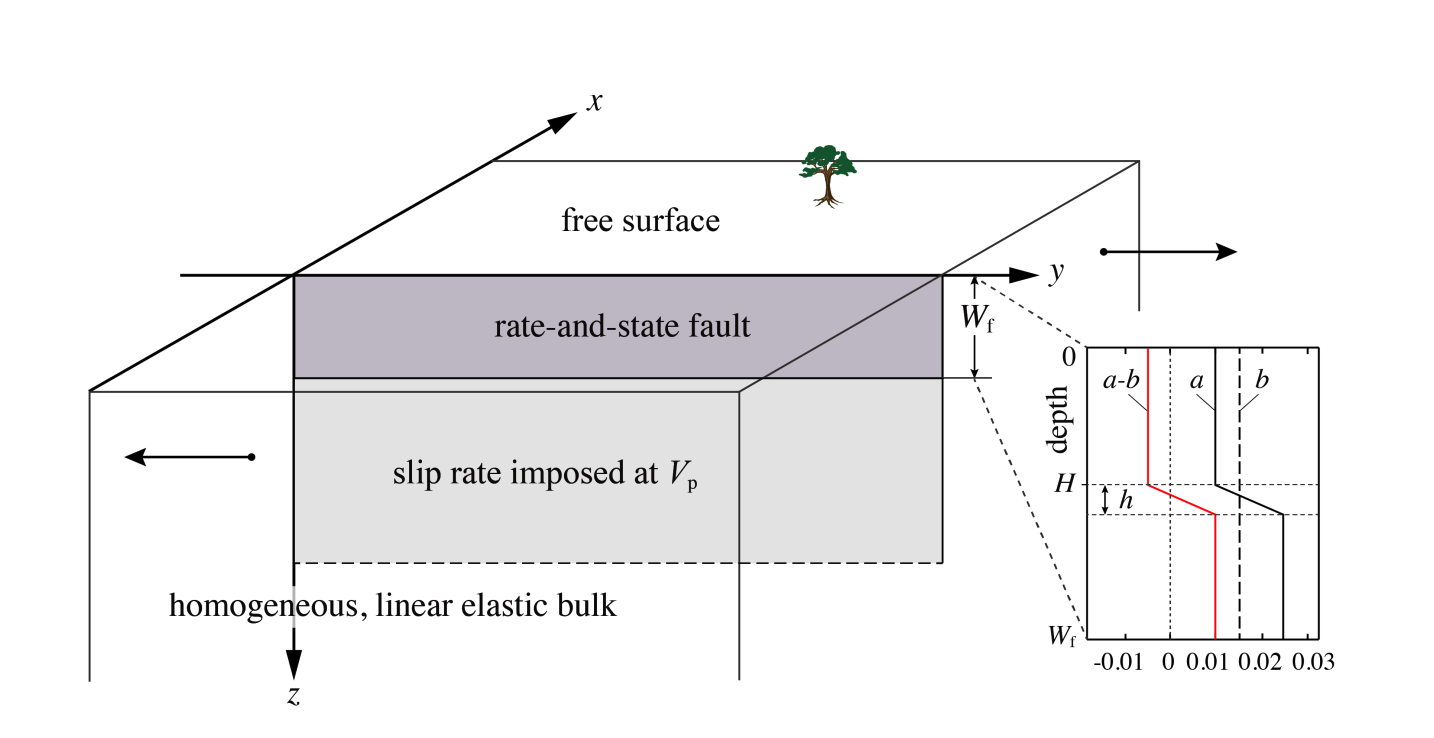
\includegraphics[width=\linewidth]{figures/BP1-figure}
    \caption{BP1 considers a planar fault embedded in a homogeneous, linear elastic halfspace with a free surface. The fault is governed by rate-and-state friction down to the depth $W_f$ and creeps at an imposed constant rate $V_p$ down to the infinite depth. The simulations will include the nucleation, propagation, and arrest of earthquakes, and aseismic slip in the post- and inter-seismic periods. The figure and the description are given in \cite{erickson2018seas}}
    \label{fig:enter-label}
\end{figure}



The 3D problem is then reduced to a 2D problem

\begin{equation}
    0 = \frac{\partial \sigma_{xy}}{\partial x} + \frac{\partial \sigma_{yz}}{\partial z}
\end{equation}
in the domain $(x,z) \in (-\infty, \infty) \times (0,\infty)$, where
\begin{equation}
    \sigma_{x,y} = \mu \frac{\partial u}{\partial x}; \quad \sigma_{yz} = \mu \frac{\partial u}{z}
\end{equation}
The above is essentially a Poisson's equation that we solve in Section 4.
The formulation of the linear system for the BP1-QD problem is similar to what is described in Chapter 4.
Instead of using methods of manufactured solutions to verify our solution and convergence, we verify our results via comparison with results from the simulations of other researchers.
The formulation of the linear systme for BP1-QD problem is similar to what is described in Chapter \label{chap:matrix-free}.
Instead of using methods of manufactured solutions to verify our solution and convergence, we verify our results via comparison with results from the simulations of other researchers.

Most parameters and boundary and initial conditions are given in the SEAS problem description. In this problem, $a$ varies with the depth
\begin{equation}
a(z) = 
\begin{cases} 
a_0, & 0 \leq z < H \\
a_0 + (a_{\text{max}} - a_0)(z - H)/h, & H \leq z < H + h \\
a_{\text{max}}, & H + h \leq z < W_\text{f} 
\end{cases}
\end{equation}
Below depth $W_f$, the fault creeps at an imposed constant rate, given by the interface condition

\begin{equation}
    V(z,t) = V_p, \quad z \geq W_\text{f}
\end{equation}

For the simulation, we discretize our problem on a 401 $\times$ 401 grid points in each direction after discretization on a 2D domain with around 160k unknowns. 
The conjugate gradient method without a preconditioner on GPUs is fast enough for the simulation to be complete in $\sim$ 2 days on a V100 GPU after solving linear system $\sim$ 300000 times.
It takes around 0.5 seconds to solve linear systems, update values, and perform other data operations.
The results for this simulation are published in \cite{erickson2023incorporating} under the model name Thrase.


\begin{figure}
    \centering
    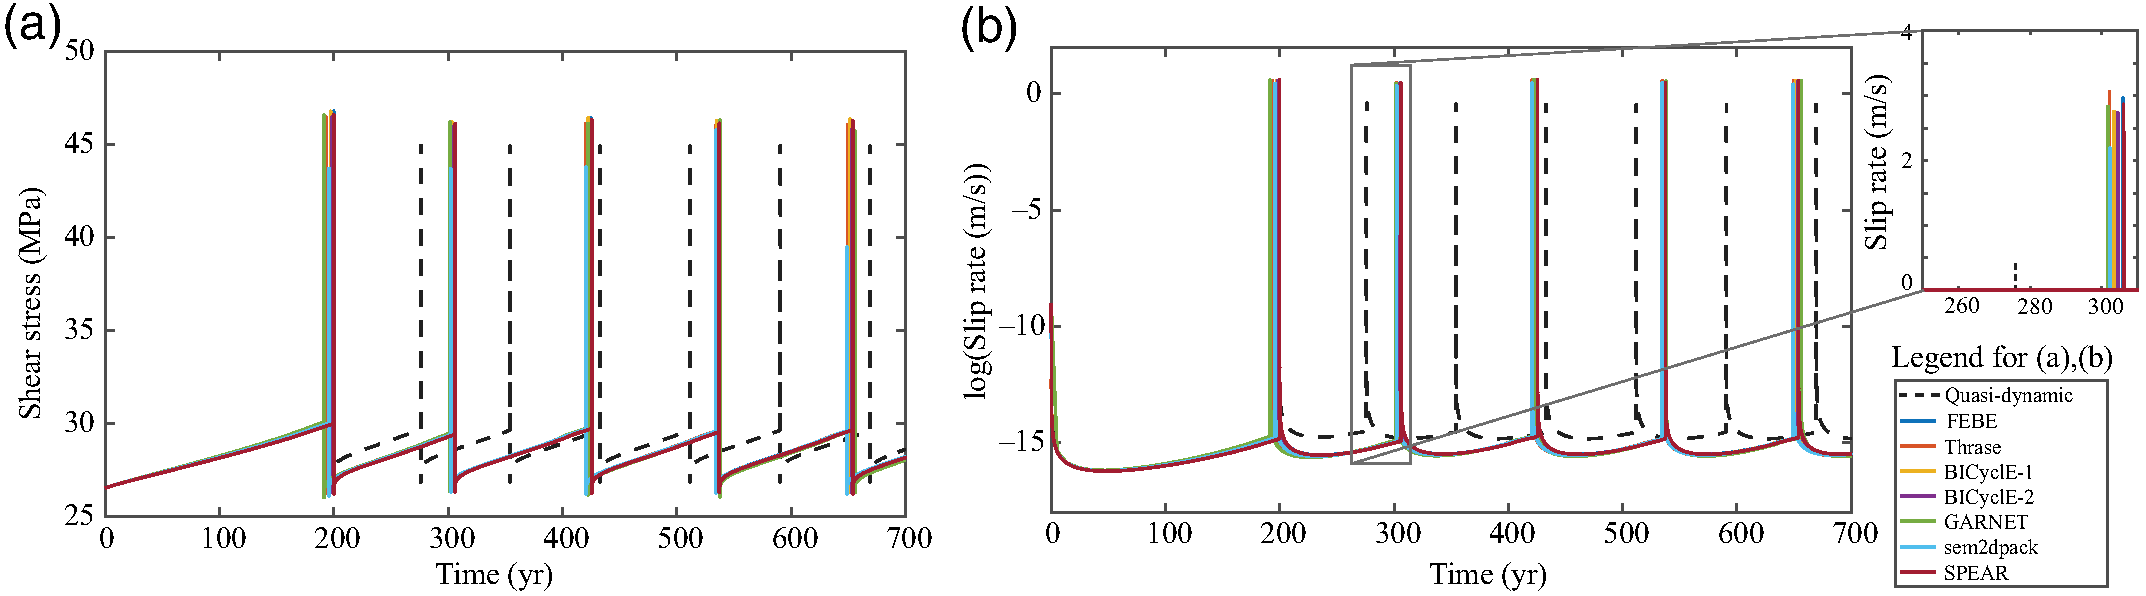
\includegraphics[width=\linewidth]{figures/BP1-seismic-plot.png}
    \caption{Long‐term behavior of BP1‐FD models. Our model name is Thrase in this figure. (a) Shear stress and (b) slip rates at the depth of 7.5 km across codes with sufficiently large computational domain sizes. Also shown (in dashed black) are those for the quasi‐dynamic counterpart BP1‐QD. The color version of this figure is available only in the electronic edition. \cite{erickson2023incorporating}}
    \label{fig:BP1-seismic-plot}
\end{figure}

The Figure \ref{fig:BP1-seismic-plot}

Figure \ref{fig:BP1-seismic-plot} shows our results along with simulation results from other researchers. 
When using different methods to solve the same benchmark problem, we achieve comparable results regarding the time between two slip events and the slip rate.


For the 2D problem with more than 1000 grid points in each direction or a 3D problem with recommended resolutions from benchmark problem 5, we will be solving linear systems with millions or tens of millions of unknowns.
The above approach is too slow even on the latest GPUs.
We need more advanced algorithms like the MGCG method described in Chapter 5.

\section{BP5-QD problem}
\subsection{Problem description}
\begin{figure}
    \centering
    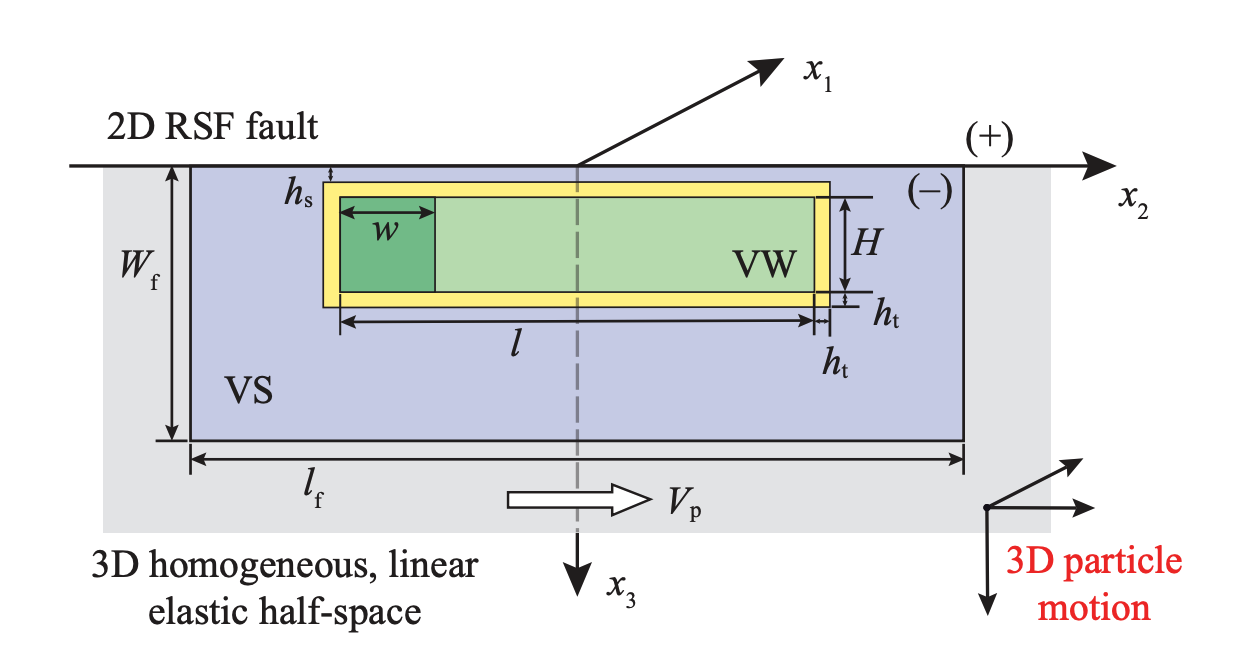
\includegraphics[width=\linewidth]{figures/BP5-figure.png}
    \caption{This benchmark considers 3D motion with a planar fault embedded vertically in a homogeneous, linear elastic whole-space. The fault is governed by rate-and-state friction in the region $0 \leq x_3 \leq W_\text{f}$ and $|x_2| \leq l_f/2$, outside of which it creeps at an imposed constant horizontal rate Vp (gray). The velocity weakening region (the rectangle in light and dark green; $h_s + h_t \leq x_3 \leq h_s + h_t + H$ and $|x_2| \leq l/2)$ is surrounded by a transition zone (yellow) of width ht to velocity strengthening regions (blue). A favorable nucleation zone (dark green square with width $w$) is located at one end of the velocity-weakening patch. \citep{jiang2020seas}}
    \label{fig:BP5-figure}
\end{figure}


\subsection{Boundary and Interface conditions}
At $x_1 = 0$, the fault defines the interfaces.
A free surface lies at $x_3 = 0$, where all components of traction have $0$ value.
This condition is written in the following form
\begin{equation}
    \sigma_{j3}(x_1, x_2, 0, t) = 0,\quad j = 1,2,3
\end{equation}
We assume a "non-opening condition" on the fault
\begin{equation}
    u_1(0^+, x_2, x_3, t) = u_1(0^-, x_2, x_3, t)
\end{equation}
For $j=2,3$, we define the slip vector as the jump in horizontal and vertical displacements across the fault.
\begin{equation}
    s_j(x_2, x_3, t) = u_j(0^+, x_2, x_3, t) - u_j(0^-, x_2, x_3, t),\quad j = 2,3
\end{equation}
We require that components of the traction vector be equal and opposite across the fault, which yields three conditions
\begin{align}
    -\sigma_{11} \left(0^+, x_2, x_3, t\right) &= -\sigma_{11} \left(0^-, x_2, x_3, t\right), \\
    \sigma_{21} \left(0^+, x_2, x_3, t\right) &= \sigma_{21} \left(0^-, x_2, x_3, t\right), \\
    \sigma_{31} \left(0^+, x_2, x_3, t\right) &= \sigma_{31} \left(0^-, x_2, x_3, t\right),
\end{align}
We denote these three common values as $\sigma$ (positive means compression), $\tau$ and $\tau_z$ respectively. 
In the simulation, $\tau$ and $\tau_z$ are key values calculated from the displacements and are used in the rate-and-state friction.
We also export the log of these two values to the output files.

Most parameters are given in the problem description. The key value is the rate-and-state friction $a$, given in the following form

\begin{equation}
    a(x_2, x_3) =
\begin{cases} 
a_0, & (h_s + h_t \leq x_3 \leq h_s + h_t + H) \cap (|x_2| \leq l/2) \\
a_{\text{max}}, & (0 \leq x_3 \leq h_s) \cup (h_s + 2h_t + H \leq x_3 \leq W_f) \\ & \cup (l/2 + h_t \leq |x_2| \leq l_f/2) \\
a_0 + r(a_{\text{max}} - a_0), & \text{other regions}
\end{cases}
\end{equation}
where $r = \max(|x_3 - h_s - h_t - H/2| - H/2, |x_2| - l/2)/h_t$.


Outside the domain $\Sigma_f$ ($|x_3| > W_\text{f}$ or $|x_2| > l_\text{f} / 2$ as denoted in the grey region in the \autoref{fig:BP5-figure}), the fault creeps horizontally at an imposed constant rate
\begin{align}
    V_2(x_2, x_3, t) &= V_\text{p} \\
    V_3(x_2, x_3, t) &= 0
\end{align}
where $V_\text{p}$ is the plate rate.

We also need to specify the initial conditions for the simulation.
We assume that slip on the fault separating identical materials does not change normal traction, so $\sigma_n$ remains constant.

The initial state and prestress on the fault is chosen so that the model can start with a uniform fault slip rate, given by $\textbf{V} = [V_\text{init}, V_\text{zero}]$ where $V_\text{zero}$ is chosen as $10^{-20}m/s$ to avoid infinite log values in the output, and $\boldsymbol{\tau}^0 = \tau^0 \textbf{V} / V$.

The initial state variable is chosen as the steady state at slip rate $V_\text{init}$ over the entire fault 
\begin{equation}
    \theta(x_2, x_3, 0) = L / V_\text{init}
\end{equation}

For the BP5-QD problem, we also need to specify an initial value for the slip, which we set to be zero.
\begin{equation}
    s_j(x_2, x_3, t) = 0, j = 2, 3
\end{equation}
The scalar pre-stress $\tau^0$ is chosen as the steady-state stress
\begin{equation}
    \tau^0 = \bar{\sigma}_\text{n} a \sinh^{-1}[\frac{V_\text{init}}{2V_0}\exp(\frac{f_0 + b\ln(V_0/V_\text{init}}{a})] + \eta V_\text{init}
\end{equation}
To break the symmetry of the problem and facilitate comparisons of different simulations, we choose a small region as a favorable location for nucleation to impose a smaller critical slip distance ($L=0.13m$) and higher initial slip rate along the $x_2$-direction ($V_i = 0.03 m/s$) while keeping the initial state variable $\theta(x_2, x_3, 0)$ unchanged. The means we impose higher pre-stress along the $x_2$-direction.

We use the recommended parameters from the problem description and perform initial simulations for 1800 years.

\subsection{SBP-SAT formulations for BP5-QD}
For this 3D problem, we use SBP-SAT methods similar to \citep{ALMQUIST2021109842} to formulate our linear system.
To solve the linear elasticity in 3D, we need to solve for the displacements in $x$, $y$, and $z$ directions for each point.
We denote the displacement vector as $\boldsymbol{u} = [u_1, u_2, u_3]$.
To turn the tensor formulation from \citep{ALMQUIST2021109842} into a matrix formulation for iterative solvers,  we first stack the displacements for a point in $x$, $y$, $z$ directions, and then for all points in $x$, $y$, and $z$ directions.
We label the faces for 3D simulation in the following order as shown in \autoref{fig:3d_problem}

\begin{figure}
    \centering
    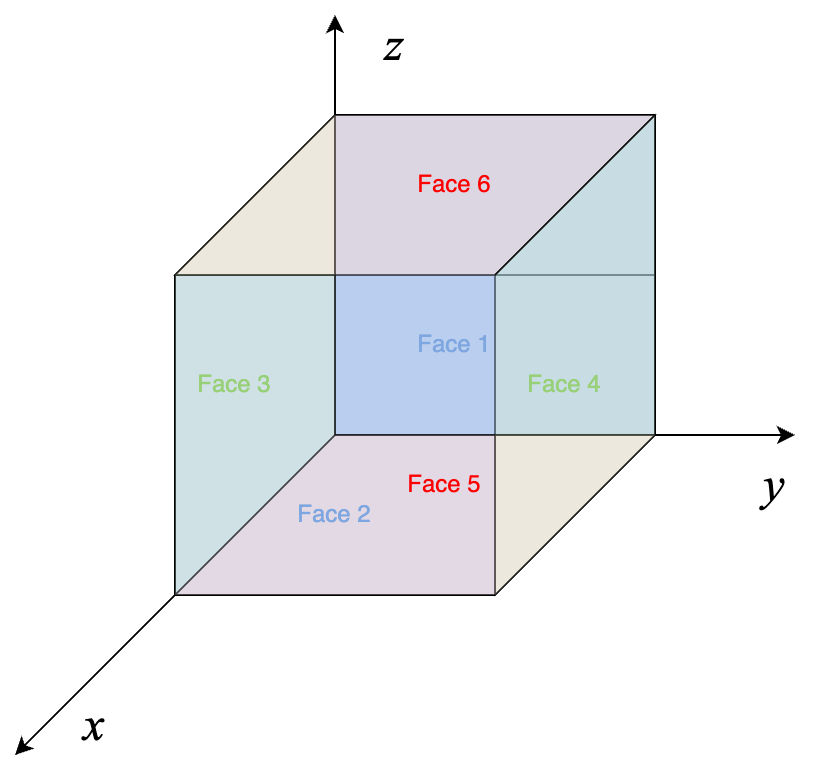
\includegraphics[width=\linewidth]{figures/3D_problem.png}
    \caption{We set up the 3D coordinate and denote faces 1 to 6 using different colors. Face 1 and Face 2 are perpendicular to the x-axis denoted using blue color. Face 3 and Face 4 are perpendicular to the y-axis denoted using green color. Face 5 and Face 6 are perpendicular to the z-axis denoted using red color. We impose Dirichlet boundary conditions on Face 1 and Face 2. For Face 3 to Face 6, we impose traction-free (Neumann) condition.} 
    \label{fig:3d_problem}
\end{figure}

The first step is to derive values for $\sigma$ tensor in 3D.

\begin{align}
    \sigma_{11} = K\epsilon_{kk} + 2\mu (\epsilon_{11} - \frac{1}{3}\epsilon_{kk}) &= (K - \frac{2}{3}\mu)( \frac{\partial u_1}{\partial x_1} + \frac{\partial u_2}{\partial x_2} + \frac{\partial u_3}{\partial x_3}) + 2\mu \frac{\partial u_1}{\partial x_1} \\
    \sigma_{12} = 2\mu \epsilon_{12} &= \mu(\frac{\partial u_1}{\partial x_2} + \frac{\partial u_2}{\partial x_1}) \\
    \sigma_{13} = 2\mu \epsilon_{13} &= \mu(\frac{\partial u_1}{\partial x_3} + \frac{\partial u_3}{\partial x_1}) \\
    \sigma_{21} = 2\mu \epsilon_{21} &= \mu(\frac{\partial u_2}{\partial x_1} + \frac{\partial u_1}{\partial x_2}) \\
    \sigma_{22} = K\epsilon_{kk} + 2\mu (\epsilon_{22} - \frac{1}{3}\epsilon_{kk}) &= (K - \frac{2}{3}\mu)( \frac{\partial u_1}{\partial x_1} + \frac{\partial u_2}{\partial x_2} + \frac{\partial u_3}{\partial x_3}) + 2\mu \frac{\partial u_2}{\partial x_2} \\
    \sigma_{23} = 2\mu \epsilon_{13} &= \mu(\frac{\partial u_2}{\partial x_3} + \frac{\partial u_3}{\partial x_2}) \\
    \sigma_{31} = 2\mu \epsilon_{31} &= \mu(\frac{\partial u_3}{\partial x_1} + \frac{\partial u_1}{\partial x_3}) \\
    \sigma_{32} = 2\mu \epsilon_{32} &= \mu(\frac{\partial u_3}{\partial x_2} + \frac{\partial u_2}{\partial x_3}) \\
    \sigma_{33} = K\epsilon_{kk} + 2\mu (\epsilon_{33} - \frac{1}{3}\epsilon_{kk}) &= (K - \frac{2}{3}\mu)( \frac{\partial u_1}{\partial x_1} + \frac{\partial u_2}{\partial x_2} + \frac{\partial u_3}{\partial x_3}) + 2\mu \frac{\partial u_3}{\partial x_3}
    \label{eqn:sigma-tensor}
\end{align}


Here, we also use $1,2,3$ to denote the components of $\sigma$ in $x,y,z$ directions to simplify the notation.
Then we can rewrite governing equations in terms of the $x,y,z$ components.

\begin{align}
    \rho \frac{\partial^2{u_1}}{\partial{t^2}} &= \frac{\partial \sigma_{11}}{\partial x_1} + \frac{\partial \sigma_{12}}{\partial x_{2}} + \frac{\partial \sigma_{13}}{\partial x_{3}} \nonumber \\
    &= (K - \frac{2}{3}\mu)( \frac{\partial^2 u_1}{\partial x_1^2} + \frac{\partial^2 u_2}{\partial x_1 \partial x_2} + \frac{\partial^2 u_3}{\partial x_1 \partial x_3}) + 2\mu \frac{\partial^2u_1}{\partial x_1^2} \nonumber \\
        & + \mu(\frac{\partial^2 u_1}{\partial x_2^2} + \frac{\partial^2u_2}{\partial x_2 \partial x_1})
        + \mu(\frac{\partial^2 u_1}{\partial x_3^2} + \frac{\partial^2u_3}{\partial x_3 \partial x_1}) \\
    \rho \frac{\partial^2{u_2}}{\partial{t^2}} &= \frac{\partial \sigma_{21}}{\partial x_1} + \frac{\partial \sigma_{22}}{\partial x_{2}} + \frac{\partial \sigma_{23}}{\partial x_{3}} \nonumber \\
    &= \mu(\frac{\partial^2u_2}{\partial x_1^2} + \frac{\partial^2 u_1}{\partial x_1 \partial x_2})
    + (K - \frac{2}{3}\mu)( \frac{\partial^2 u_1}{\partial x_2 \partial x_1} + \frac{\partial^2 u_2}{\partial x_2^2} + \frac{\partial^2 u_3}{\partial x_2 \partial x_3}) \nonumber \\
    &+ 2\mu \frac{\partial^2u_2}{\partial x_2^2} 
    + \mu(\frac{\partial^2u_2}{\partial x_3^2} + \frac{\partial^2 u_3}{\partial x_3 \partial x_2}) \\
    \rho \frac{\partial^2{u_3}}{\partial{t^2}} & = \frac{\partial \sigma_{31}}{\partial x_1} + \frac{\partial \sigma_{32}}{\partial x_{2}} + \frac{\partial \sigma_{33}}{\partial x_{3}} \nonumber \\
    &= \mu(\frac{\partial^2u_3}{\partial x_1^2} + \frac{\partial^2 u_1}{\partial x_1 \partial x_3}) \nonumber
    + \mu(\frac{\partial^2 u_3}{\partial x_2^2} + \frac{\partial^2u_2}{\partial x_2 \partial x_3}) \\
    & + (K - \frac{2}{3}\mu)( \frac{\partial^2 u_1}{\partial x_3 \partial x_1}   + \frac{\partial^2 u_2}{\partial x_3 \partial x_2} + \frac{\partial^2 u_3}{\partial x_3^2}) + 2\mu \frac{\partial^2u_3}{\partial x_3^2} 
    \label{eqn:components}
\end{align}

We can use them to impose the SAT terms for displacements in $x, y, z$ directions using formulations from \citep{ALMQUIST2021109842}.
For Neuman boundary conditions, we have
\begin{align}
    SAT_1 = &-H^{-1} [e_3 H_3 (e_3^T [T_{11}^3 u_1 + T_{12}^3 u_2 + T_{13}^3 u_3] - g_1^3)] \nonumber \\
&- H^{-1} [e_4 H_4 (e_4^T [T_{11}^4 u_1 + T_{12}^4 u_2 + T_{13}^4 u_3] - g_1^4)] \nonumber \\
&- H^{-1} [e_5 H_5 (e_5^T [T_{11}^5 u_1 + T_{12}^5 u_2 + T_{13}^5 u_3] - g_1^5)] \nonumber \\
&- H^{-1} [e_6 H_6 (e_6^T [T_{11}^6 u_1 + T_{12}^6 u_2 + T_{13}^6 u_3] - g_1^6)] \\
SAT_2 = &-H^{-1} [e_3 H_3 (e_3^T [T_{21}^3 u_1 + T_{22}^3 u_2 + T_{23}^3 u_3] - g_2^3)] \nonumber \\
& - H^{-1} [e_4 H_4 (e_4^T [T_{21}^4 u_1 + T_{22}^4 u_2 + T_{23}^4 u_3] - g_2^4)] \nonumber \\
& - H^{-1} [e_5 H_5 (e_5^T [T_{21}^5 u_1 + T_{22}^5 u_2 + T_{23}^5 u_3] - g_2^5)] \nonumber \\
& - H^{-1} [e_6 H_6 (e_6^T [T_{21}^6 u_1 + T_{22}^6 u_2 + T_{23}^6 u_3] - g_2^6)] \\
SAT_3 = &-H^{-1} [e_3 H_3 (e_3^T [T_{31}^3 u_1 + T_{32}^3 u_2 + T_{33}^3 u_3] - g_3^3)] \nonumber\\
& - H^{-1} [e_4 H_4 (e_4^T [T_{31}^4 u_1 + T_{32}^4 u_2 + T_{33}^4 u_3] - g_3^4)] \nonumber\\
& - H^{-1} [e^5 H_5 (e_5^T [T_{31}^5 u_1 + T_{32}^5 u_2 + T_{33}^5 u_3] - g_3^5)] \nonumber\\
& - H^{-1} [e^6 H_6 (e_6^T [T_{32}^6 u_1 + T_{32}^6 u_2 + T_{33}^6 u_3] - g_3^6)]
\label{eqn:neumann-condition}
\end{align}

For Dirichlet conditions, we have
\begin{align}
    \tilde{SAT_1} &= H^{-1} (T_{11}^1 - Z_{11}^1)^T e_1 H_1 (e_1^T u_1 - g_1^1) \nonumber \\
    &+ H^{-1} (T_{21}^1 - Z_{21}^1)^T e_1 H_1 (e_1^T u_2 - g_2^1) \nonumber\\ 
    &+ H^{-1} (T_{31}^1 - Z_{31}^1)^T e_1 H_1 (e_1^T u_3 - g_3^1) \nonumber\\
    &+ H^{-1} (T_{11}^2 - Z_{11}^2)^T e_2 H_2 (e_2^T u_1 - g_1^2) \nonumber\\
    &+ H^{-1} (T_{21}^2 - Z_{21}^2)^T e_2 H_2 (e_2^T u_2 - g_2^2) \nonumber\\
    &+ H^{-1} (T_{31}^2 - Z_{31}^2)^T e_2 H_2 (e_2^T u_3 - g_3^2) \\
    \tilde{SAT_2} &= H^{-1} (T_{12}^1 - Z_{12}^1)^T e_1 H_1 (e_1^T u_1 - g_1^1) \nonumber \\
    & + H^{-1} (T_{22}^1 - Z_{22}^1)^T e_1 H_1 (e_1^T u_2 - g_2^1) \nonumber \\
    & + H^{-1} (T_{32}^1 - Z_{32}^1)^T e_1 H_1 (e_1^T u_3 - g_3^1) \nonumber \\
    & + H^{-1} (T_{12}^2 - Z_{12}^2)^T e_2 H_2 (e_2^T u_1 - g_1^2) \nonumber \\
    & + H^{-1} (T_{22}^2 - Z_{22}^2)^T e_2 H_2 (e_2^T u_2 - g_2^2) \nonumber \\ 
    & + H^{-1} (T_{32}^2 - Z_{32}^2)^T e_2 H_2 (e_2^T u_3 - g_3^2) \\
    \tilde{SAT_3} &= H^{-1} (T_{13}^1 - Z_{13}^1)^T e_1 H_1 (e_1^T u_1 - g_1^1) \nonumber \\
    & + H^{-1} (T_{23}^1 - Z_{23}^1)^T e_1 H_1 (e_1^T u_2 - g_2^1) \nonumber \\ 
    & + H^{-1} (T_{33}^1 - Z_{33}^1)^T e_1 H_1 (e_1^T u_3 - g_3^1) \nonumber \\
    & + H^{-1} (T_{13}^2 - Z_{13}^2)^T e_2 H_2 (e_2^T u_1 - g_1^2) \nonumber \\
    & + H^{-1} (T_{23}^2 - Z_{23}^2)^T e_2 H_2 (e_2^T u_2 - g_2^2) \nonumber \\
    & + H^{-1} (T_{33}^2 - Z_{33}^2)^T e_2 H_2 (e_3^T u_3 - g_3^2)
    \label{eqn:dirichlet-condition}
\end{align}


% \subsection{Discretization and parameters selection}


\subsection{Results}
We discretize the problem on a truncated 128km $\times$ 128km $\times$ 128 km domain. The simulation parameters are chosen to be the values in \citep{jiang2020seas}. 
We export results on stations on the fault according to the problem description. We run our simulations for 1800 years and compare our results with results from other researchers on similar problems.

We compare our results using BEMs from Cattania's group. This method only requires solving problems on the fault surface, and does not require domain truncation. Previous results have shown that domain truncation in volume-based methods would affect earthquake cycles
We first look at the changes in shear stress along the slip direction for a sample location on the fault. We compare our results with Cattania's group using boundary element methods and plot the result in \autoref{fig:bp5-shearstress}. We see similar ranges of state variables and similar behaviors of jumps in state variables during the transition between aseismic slips and seismic slips. We then compare the slip for the same location on the fault and plot them in \autoref{fig:bp5-slip2}.

\begin{figure}
    \centering
    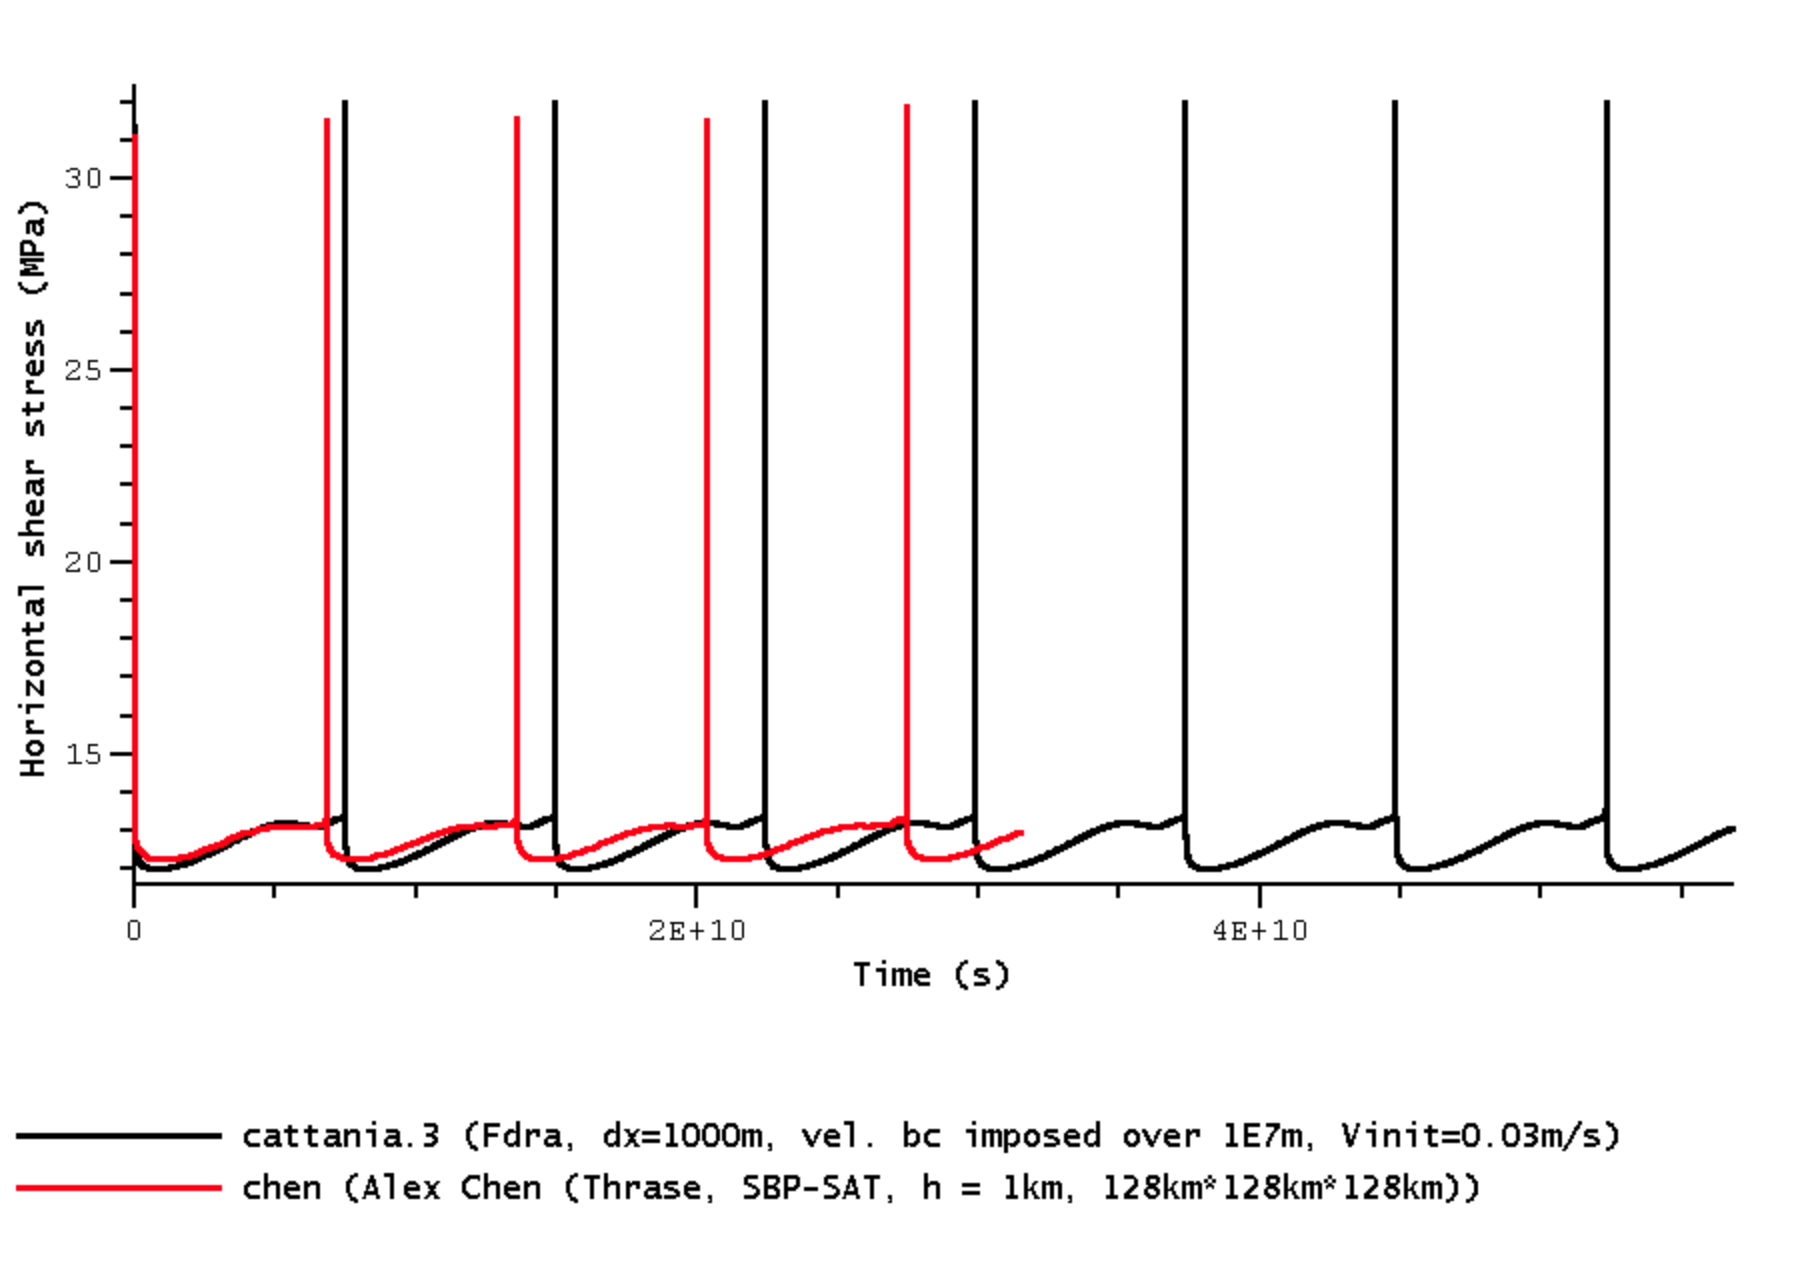
\includegraphics[width=\linewidth]{figures/sample-shearstress.png}
    \caption{Comparison of shear stress along slip directions}
    \label{fig:bp5-shearstress}
\end{figure}

\begin{figure}
    \centering
    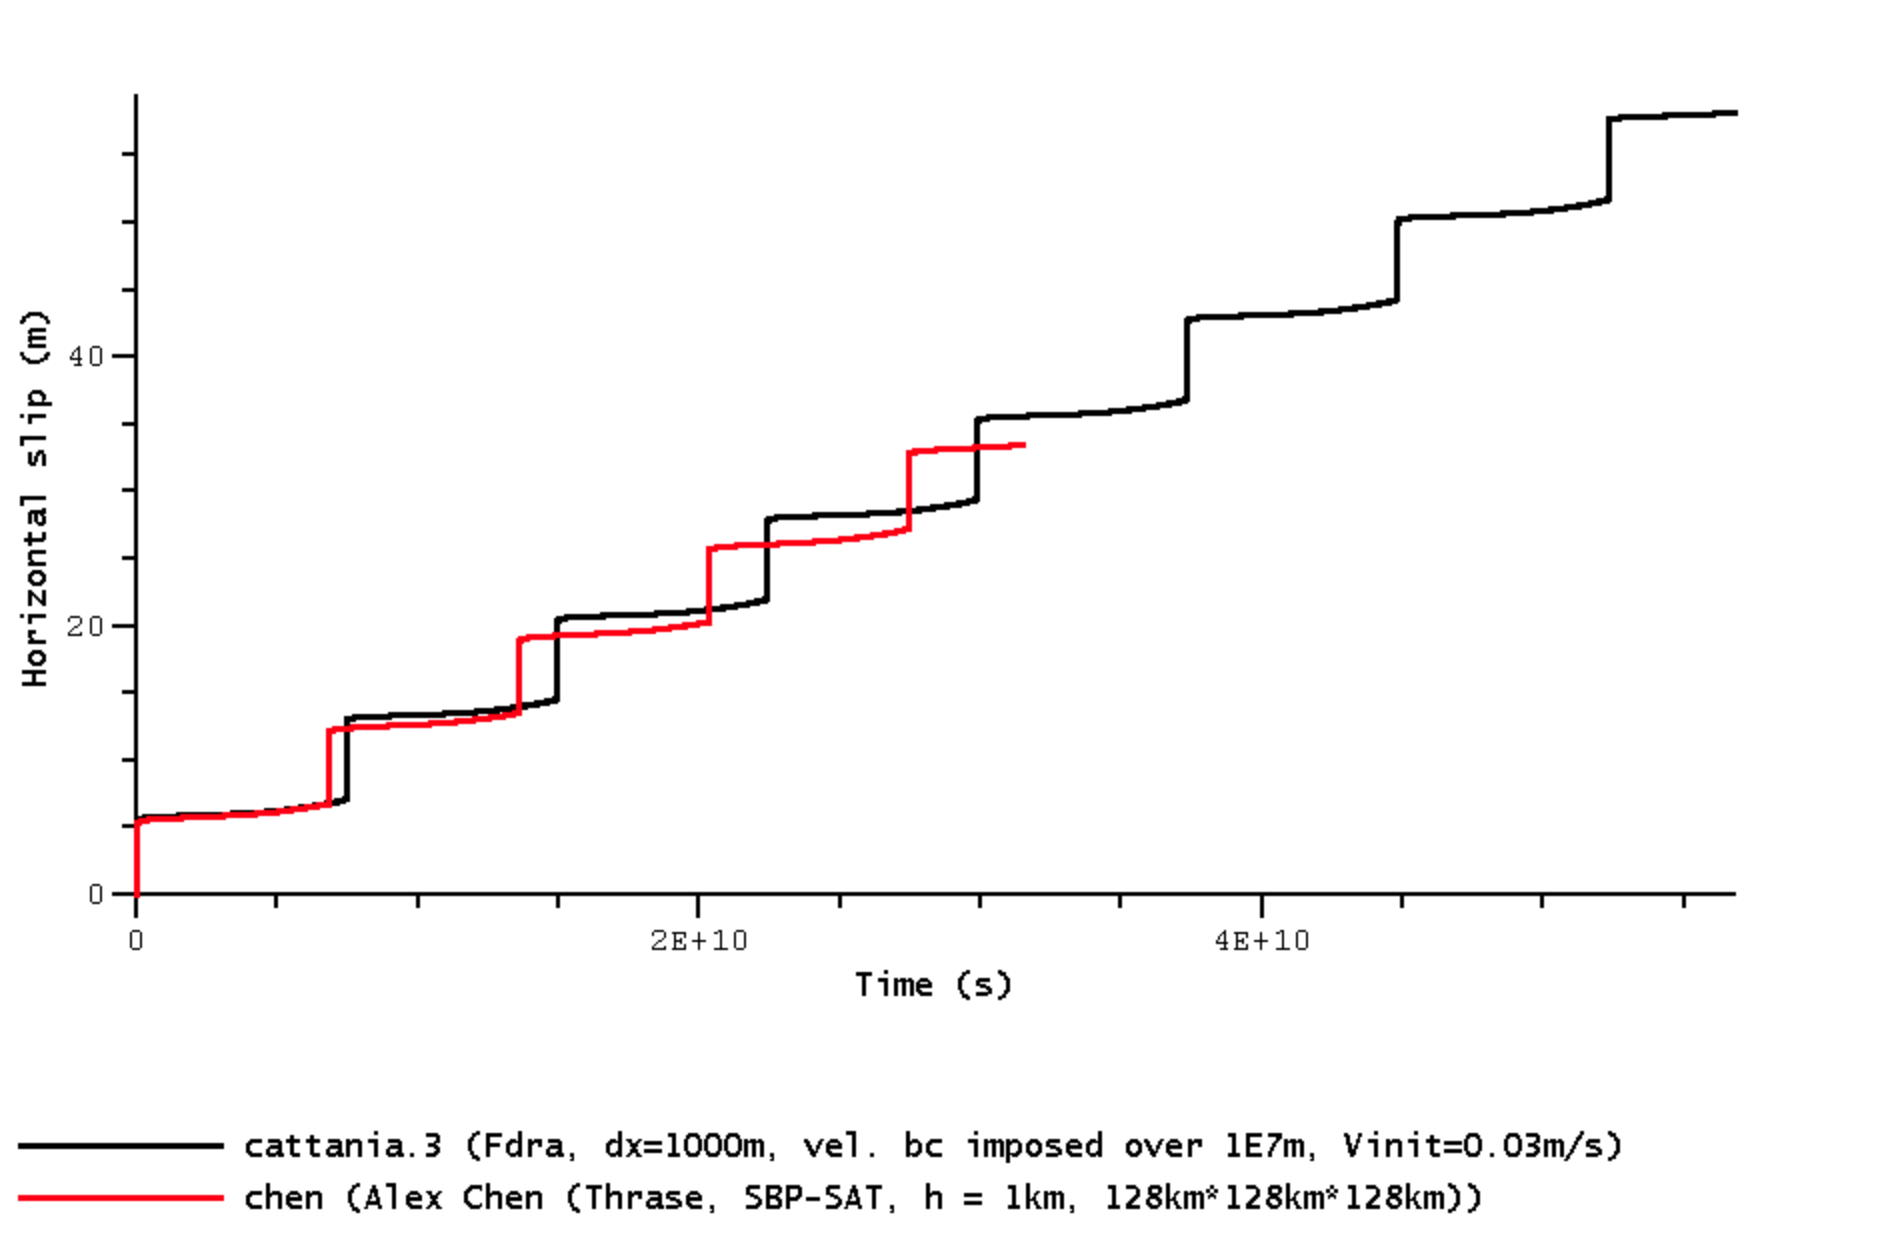
\includegraphics[width=\linewidth]{figures/sample-slip-2.png}
    \caption{Comparison of shear stress along slip directions}
    \label{fig:bp5-slip2}
\end{figure}

Preliminary results have shown agreement in the modeling of the same problems using different methods.
Current results from other simulations are mainly based on boundary element methods, which take hours to run.
Our methods are volume-based and have more than 100 times higher degrees of freedom.
With the GPU-accelerated MGCG as a solver, our simulation time is cut to around ~8 hours, with around $0.2s$ for each round of solving linear system and updating values. 
This is down from weeks and months of estimated time using direct methods if we have sufficient large enough memory for matrix factorization.

%--- Chapter 6 ----------------------------------------------------------------%
\chapter{Conclusion}
% \section{Chapter Four Section One}
% \subsection{Chapter four section one sub-section one}
% \subsubsection{Chapter four section one sub-section one sub-sub-section one}
\section{Conclusion}
In this thesis, I present the research work during my PhD to apply HPC methods to earthquake cycle simulations.
In particular, I focus on designing efficient iterative solvers for the numerically stable SBP-SAT finite difference methods.
There are mainly two novel contributions of the work. Firstly, I design matrix-free GPU kernels for SBP-SAT methods based on traditional stencil computation. Secondly, I designed a geometric multigrid preconditioner that is compatible with my matrix-free GPU kernels based on the existing work of the SBP-preserving interpolation operators.
The combined approach has been proven efficient in solving linear systems formed with the SBP-SAT methods, and we are outperforming the state-of-the-art implementations from well-known scientific computing libraries and proprietary software.
We then apply this approach to solving SEAS modeling problems and achieve more than 100x speedup compared to traditional methods.
More importantly, this approach is memory efficient that allows us to solve a 3D simulation problem formulated with the SBP-SAT method that can not be solved by factorization-based direct methods. 
The work presented in this thesis is valuable not only to Earth science research but also to numerous other scientific fields where SBP-SAT methods can be applied.
\section{Future Work}
This work is focused on the second-order SBP-SAT methods. SBP-SAT methods are known to be high order accuracy, and using higher-order SBP operators will increase arithmetic intensity that will increase the performance of matrix-free GPU kernels compared to SpMV operators.

In addition, the matrix-free kernels presented in this paper are only implemented on a single GPU. 
Although this is enough to solve the problems presented in this paper, it would be more important in the HPC aspect to design matrix-free kernels that can run on multiple GPUs across different nodes.
ParallelStencils.jl is a Julia package that enables large-scale stencil-based computations using built-in modules that utilize MPI for communication.
It's also built on top of KernelAbstractions.jl, a Julia package that targets heterogeneous platforms.
Our code on matrix-free SBP-SAT methods can be developed with ParallelStencils.jl to run on supercomputers built with CPUs/GPUs from different vendors.

In this work, we only apply Richardson iteration as matrix-free smoothers for our multigrid preconditioners. During our research, we observed faster convergence with higher-order Krylov subspace methods as smoother. These methods are also highly suitable for GPU architectures and can be implemented matrix-free.
In future work, we can explore using higher order second-order Richardson methods and Chebyshev iterations as smoothers in multigrid methods to further reduce steps till convergence for CG.
